\setcounter{chapter}{9-1} %Makes the prereq chapter chapter 0

\chapter{Non-parametric Methods}

    \subsection{Parametric Methods}

        We've spent a large part of the course on models that rely on \purp{parameters}:
    
        \begin{itemize}
            \item Linear regression/classification models, with parameters $\blu{\Theta} = \big( \blu{\theta}, \blu{\theta_0} \big)$:
    
            \begin{equation}
                h(x; \blu{\Theta}) = \blu{\theta}^Tx + \blu{\theta_0}
            \end{equation}
    
            \item Neural networks, with weights $W^\ell$ and $W^\ell_0$:
    
            \begin{equation}
                \pur{A^\ell} = f(\org{Z^\ell})
                \qquad \qquad 
                \org{Z^\ell} =
                    (\blu{W^\ell})^T \red{A^{\ell-1}} + \blu{W_0^\ell} 
            \end{equation}
        \end{itemize}
    
        These can be thought of as "parametric" methods:\\
    
        \begin{definition}
            \vocab{Parametric methods} are those with a \purp{fixed number of parameters}.
    
            \begin{itemize}
                \item Typically, we optimize these models by \gren{changing} those parameters.
            \end{itemize}
    
            We can also phrase these as "models with a particular, known mathematical form".
        \end{definition}
    
        \miniex The equation $y=mx+b$ has the \orgg{fixed} parameters $m$ and $b$. It assumes our data will follow the "mathematical form" of a line.
    
        \begin{figure}[H]
            \centering
            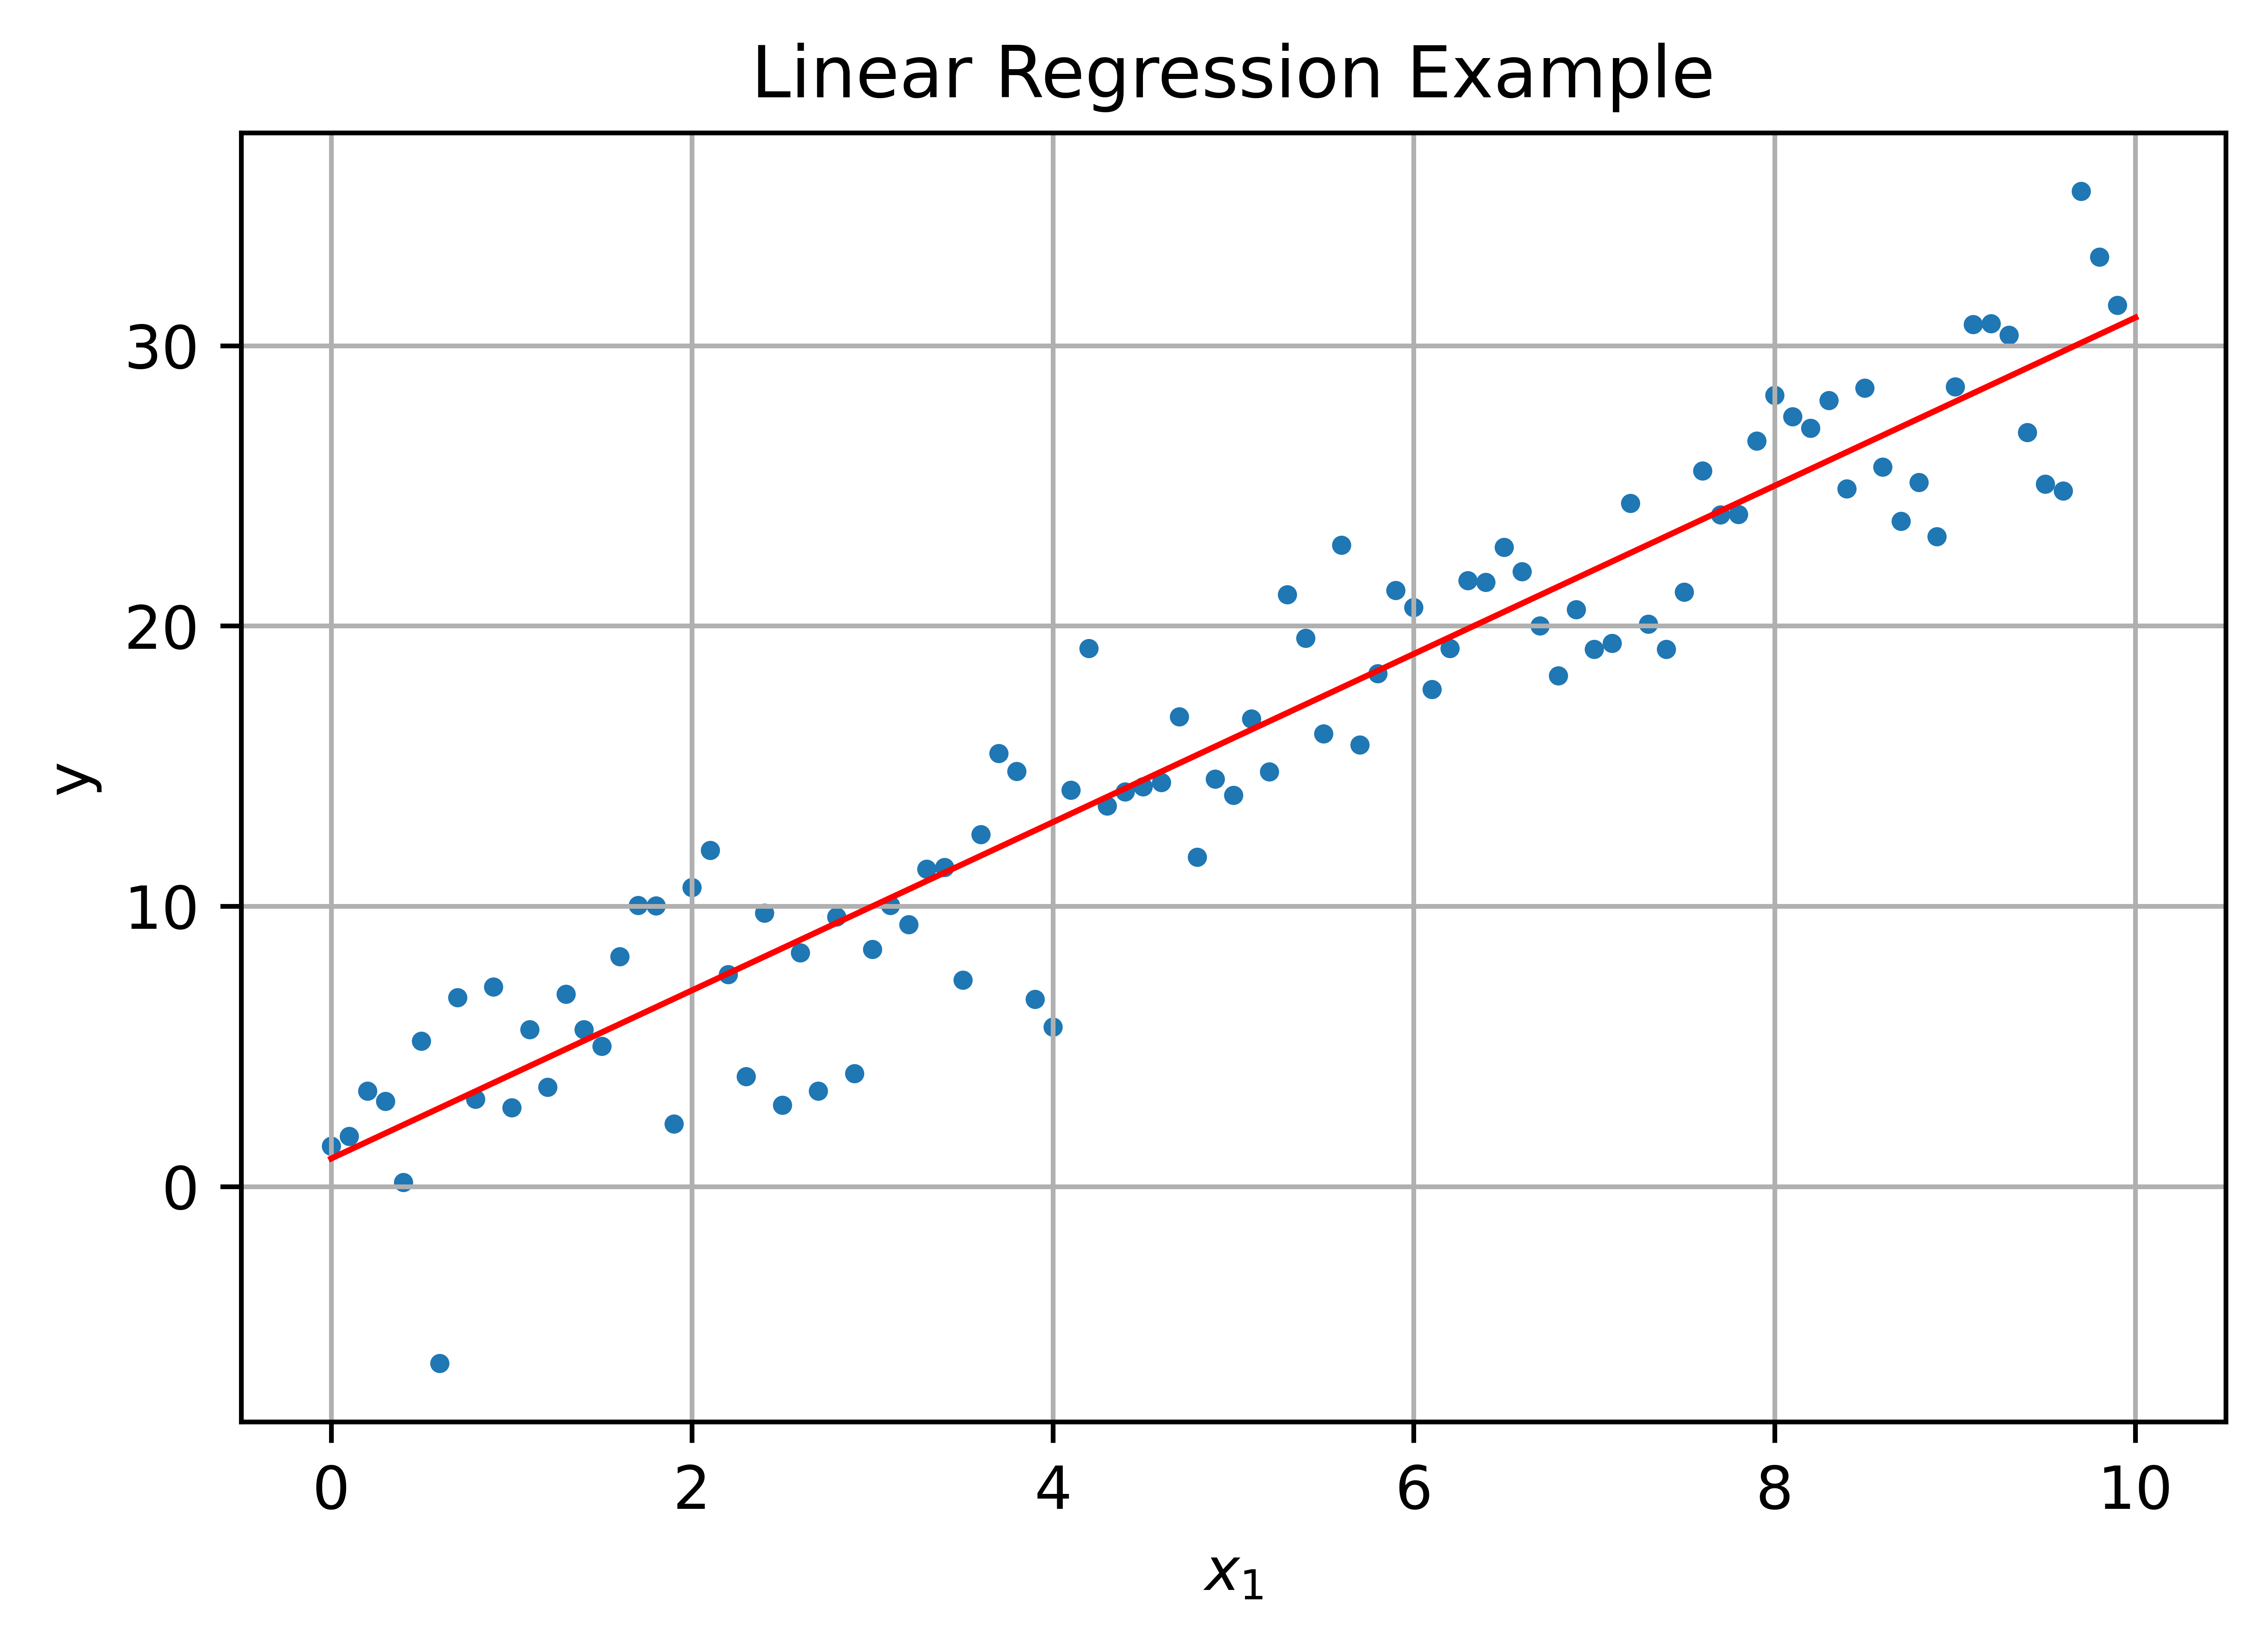
\includegraphics[width=70mm,scale=0.5]{images/regression_images/Regression_Example_Good_Fit.png}
        
            \caption*{This kind of model works best if the "true distribution" follows a similar shape.}
        \end{figure}
    
        Neural networks have the advantage of being very \vocab{expressive}: they can express \orgg{many different} kinds and distributions of data.

        \begin{itemize}
            \item The same NN architecture can be re-used to make tools for multiple different tasks.
                \note{And if our problem is too complex, we can systematically increase expressiveness: increase layer size and depth.
            
                \phantom{}
                
                We should be careful adding layers blindly, though.}
            
        \end{itemize}
            
    
        These methods have been our primary focus, because they're very configurable, and have a wide range of applications.

        But they aren't our only option.



    \phantom{}

    \subsection{Non-parametric methods}

        We can consider models that are more \textit{flexible}. Rather than assuming a particular structure, we can discover patterns, directly from our data.\\
    
        \begin{definition}
            \vocab{Non-parametric methods} \textit{exclude} models with a \orgg{fixed number} of parameters. 
            
    
            Instead, it includes:
    
            \begin{itemize}
                \item Models with \purp{no parameters}
                \item Models with a \gren{variable number of parameters}, depending on the data.
            \end{itemize}
    
            The name can be misleading: non-parametric models \textit{can} have parameters!
        \end{definition}
    
        As suggested in our definition, these methods often base their structure on the data they receive.

        Here are some \purp{examples}, each with a unique, \gren{data-based} model structure:

        \begin{itemize}
            \item \vocab{$k$-means clustering}: We already discussed this in the \purp{Clustering} chapter! 
                \note{Note that $k$ isn't a parameter: it's a \textit{hyperparameter}.} 

                \begin{itemize}
                    \item We want to cluster our training data as tightly (low-variance) as possible.
                \end{itemize}

            
            \item \vocab{Nearest neighbor}: We predict the output $\ex{g}{i}$ of a data point $\ex{x}{i}$, based on the \gren{nearest} points of training data.
                \note{Reminder: $\ex{y}{i}$ is the true value, $\ex{g}{i}$ is our prediction.}

                \begin{itemize}
                    \item In this case, we \purp{don't have} a model at all: we just directly use our data.
                \end{itemize}
            
            \item \vocab{Tree models}: We \gren{split} up our space into smaller pieces. Each region of inputs is assigned an output $y$.

                \begin{itemize}
                    \item We divide up space to get good accuracy on training data.
                \end{itemize}
            
        \end{itemize}

        And here are some examples that \orgg{combine} many simpler models, in a non-parametric way:

        \begin{itemize}
            \item \vocab{Ensembles}: We train multiple models on the whole data set, and we \purp{average} them.

            \begin{itemize}
                \item By combining multiple models, they'll (hopefully) average out to being more accurate, reducing estimation error.
                    \note{We'll specifically refer to "bagging" in this chapter.}
            \end{itemize}
            
            \item \vocab{Boosting}: in boosting, we use multiple models \gren{consecutively}: we train one model, and then we use our second model to try to improve on the mistakes of the first.

            \begin{itemize}
                \item If an earlier model struggled with a data point, that data point is \purp{weighted more heavily}: future models will focus more on that mistake.
                \item We will not discuss boosting further.
            \end{itemize}
            
        \end{itemize}





    
    
    \phantom{}

    
    \subsection{Why learn about non-parametric methods?}

        Of course, neural networks are incredibly popular for a reason: they're \purp{effective} at what they do.

        So, why do we need non-parametric methods? Well, they come with several major benefits:\\

        \begin{concept}
            \vocab{Non-parametric methods} can have genuine benefits over parametric, \purp{neural network} models:

            \begin{itemize}
                \item Fast to \gren{implement}, few hyperparameters to tune.
                
                \item Often \orgg{human-interpretable}, easier to understand than a neural network computation.

                \item In some circumstances, \purp{just as well or better} than neural networks, despite their relative simplicity.
            \end{itemize}
        \end{concept}


    \pagebreak




    

    





\section{Nearest Neighbor}

    Suppose that you're trying to figure out how to approach a problem. Maybe a medical problem, or just a personal situation with a friend.
    
    \begin{itemize}
        \item One question you can ask yourself is, "what's the most \gren{similar} situation I can think of?"
        \item If that's not enough, you could think of 2, or 3, similar examples, and try to \orgg{guess} from that, what the best course of action is.
    \end{itemize}

    This is the basic idea of the \vocab{nearest neighbor} approach: we have a new data point. We want to use the most similar examples from our past \gren{training data} to make a judgment.

    \begin{itemize}
        \item We judge the most relevant/"similar" data based on lowest \purp{distance}: we call this the "nearest neighbor".
    \end{itemize}

    What's interesting is that we're \textbf{not} developing a model: we're directly using our training data to make predictions.

    In the simplest variation, we only choose the \orgg{single closest data point}.\\

    \begin{definition}
        \vocab{Nearest neighbor method} is a \purp{non-parametric} method where we predict output $\ex{g}{i}$ based on the \orgg{nearest} data point (\vocab{nearest neighbor}) in our training set.

        \begin{itemize}
            \item Our assumption is that nearby data points are \gren{similar} to the situation we're currently dealing with.
            \item So, they should have similar \purp{outcomes}.
        \end{itemize}

        This method works \orgg{exactly the same} for regression and classification:

        \begin{itemize}
            \item Whatever output $\ex{g}{i}$ we find for the nearest neighbor, is our \purp{prediction} for our data point.
        \end{itemize}
    \end{definition}

    One nice benefit of nearest neighbor is that we require no training: we just check the training data, to make a judgment.\\
    
    \begin{concept}
        \vocab{Nearest-neighbor models} don't require training: you directly reference the training data to come to answers.
    \end{concept}

    \phantom{}

    \subsection{Nearest Neighbors: An example}

        Consider this classification problem. 
    
        \begin{figure}[H]
            \centering
            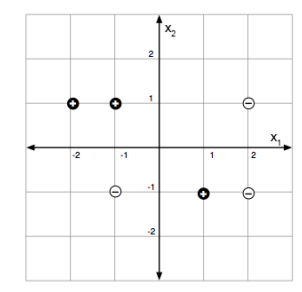
\includegraphics[width=50mm,scale=0.5]{images/nonparametric_images/classification_example.png}
        \end{figure}
        
        Rather than use a linear model, we'll assign any data point to the \gren{same class} as whichever data point it's closest to.
    
        \begin{figure}[H]
            \centering
            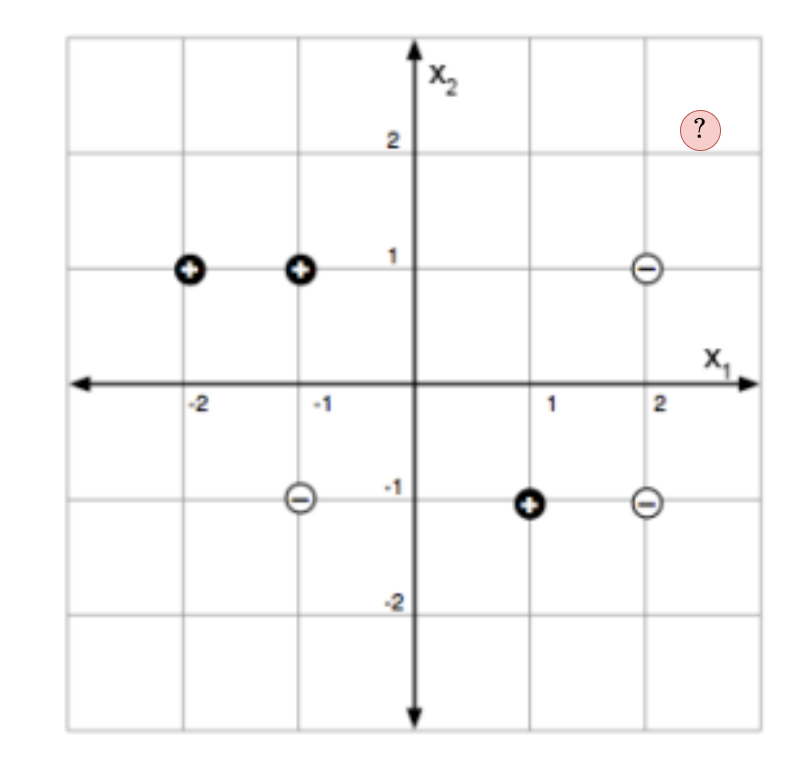
\includegraphics[width=50mm,scale=0.5]{images/nonparametric_images/mystery_datapoint.png}
            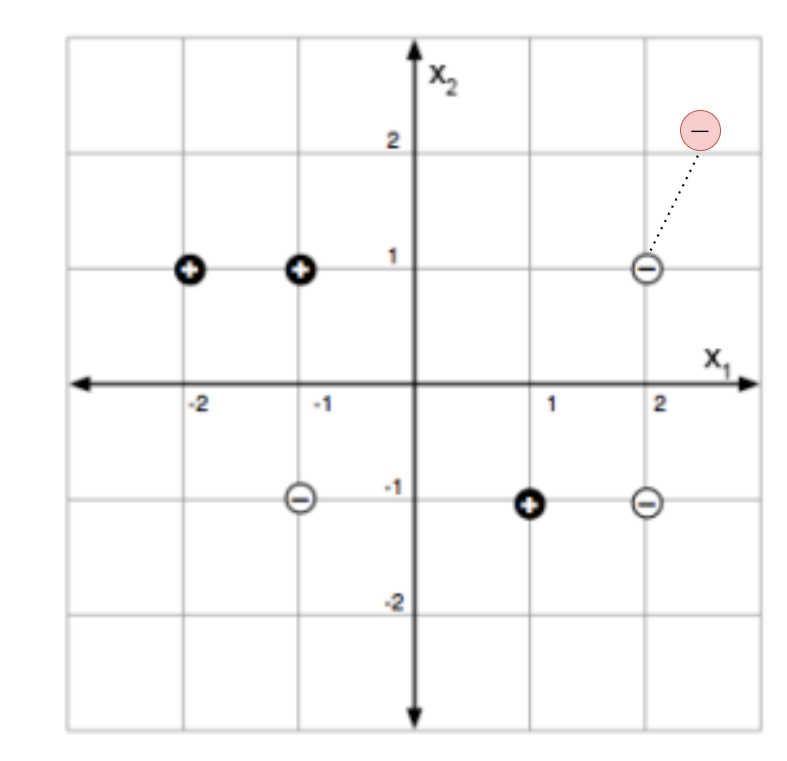
\includegraphics[width=50mm,scale=0.5]{images/nonparametric_images/mystery_assigned.png}
            \caption*{This red data point is closest to a negative data point. So, we'll assign it negative.}
        \end{figure}
    
        We could apply this to as many data points as we want:
    
        \begin{figure}[H]
            \centering
            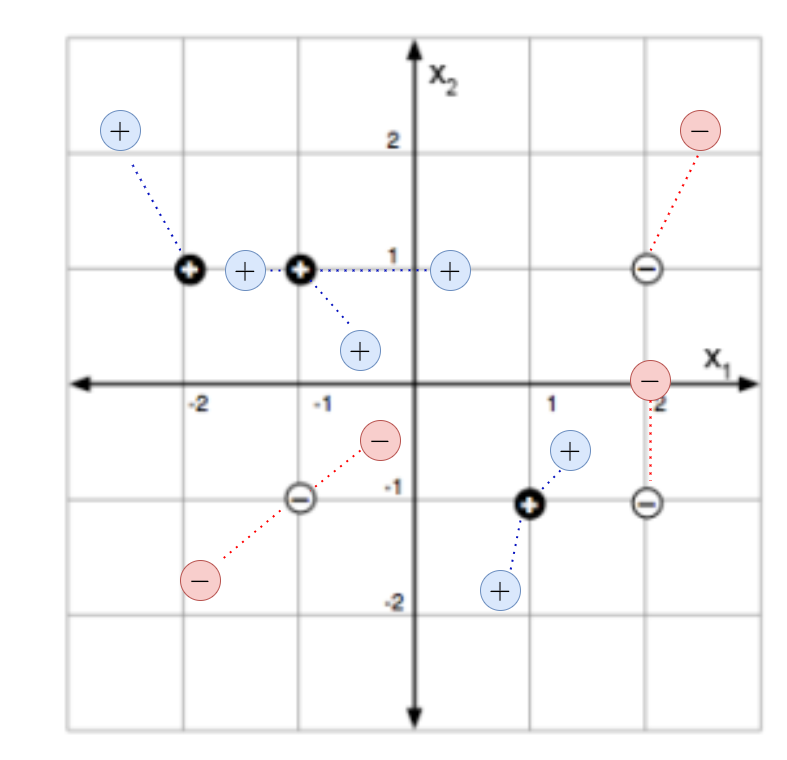
\includegraphics[width=50mm,scale=0.5]{images/nonparametric_images/many_data_nearest_neighbor.png}
    
            \caption*{We can see all of the data points that we assign our nearest neighbor to.}
        \end{figure}
    
        We're starting to fill the space: we see that some whole "\orgg{regions}" are positive or negative. 
        
        \begin{itemize}
            \item We can even depict that: we'll highlight the regions which are labelled positive vs. negative.
        \end{itemize}
    
        \begin{figure}[H]
            \centering
            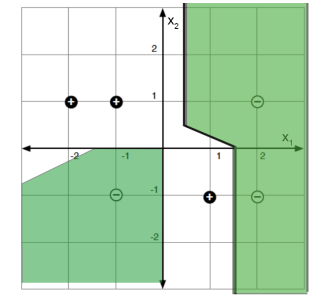
\includegraphics[width=50mm,scale=0.5]{images/nonparametric_images/nearest_neighbor.png}
    
            \caption*{We can see all of the data points that we assign our nearest neighbor to. Negative regions are green.}
        \end{figure}


    \phantom{}

    \subsection{Simplified Voronoi Diagram (\redd{Optiona})}

        This kind of diagram lets you classify data very quickly. It would be useful to be able to draw:\\
    
        \begin{concept}
            To help with finding \vocab{nearest-neighbor classification boundaries}, it can be helpful to draw a line \purp{halfway} between opposite-label data points, $A$ and $B$.
            
            \begin{itemize}
                \item This is where the distance to either data point is \gren{equal}. 
                \item We decide output based on closeness to $A$ or $B$, so this a \orgg{decision boundary}.
            \end{itemize}

            \subsecdiv

            In order to split the space between "closer to point $A$" and "closer to point $B$", we'll draw a boundary line \purp{perpendicular to} the line from $A$ to $B$.
        \end{concept}

        \begin{figure}[H]
            \centering
            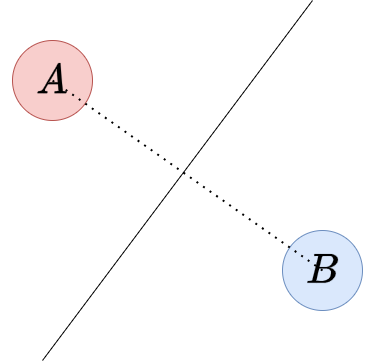
\includegraphics[width=20mm,scale=0.5]{images/nonparametric_images/simple_perpendicular.png}
    
            \caption*{We drew a solid line, where the entire line is equally far from points $A$ and $B$. Notice that it is 1. halfway between them and 2. perpendicular to the line from $A$ to $B$.}
        \end{figure}

        If we apply this to our previous problem:

        \begin{figure}[H]
            \centering
            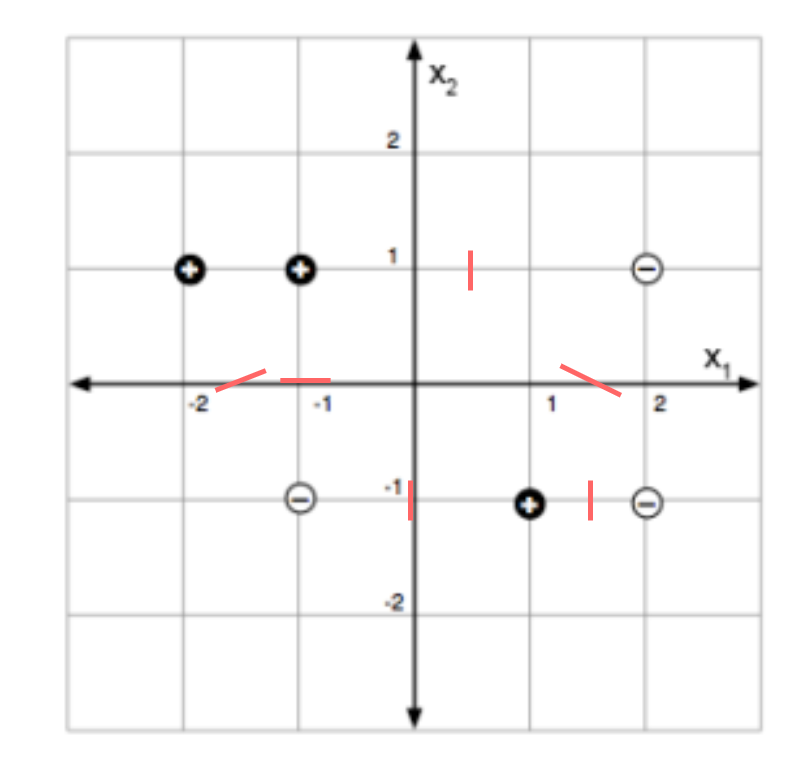
\includegraphics[width=40mm,scale=0.5]{images/nonparametric_images/nn_perpendicular.png}
            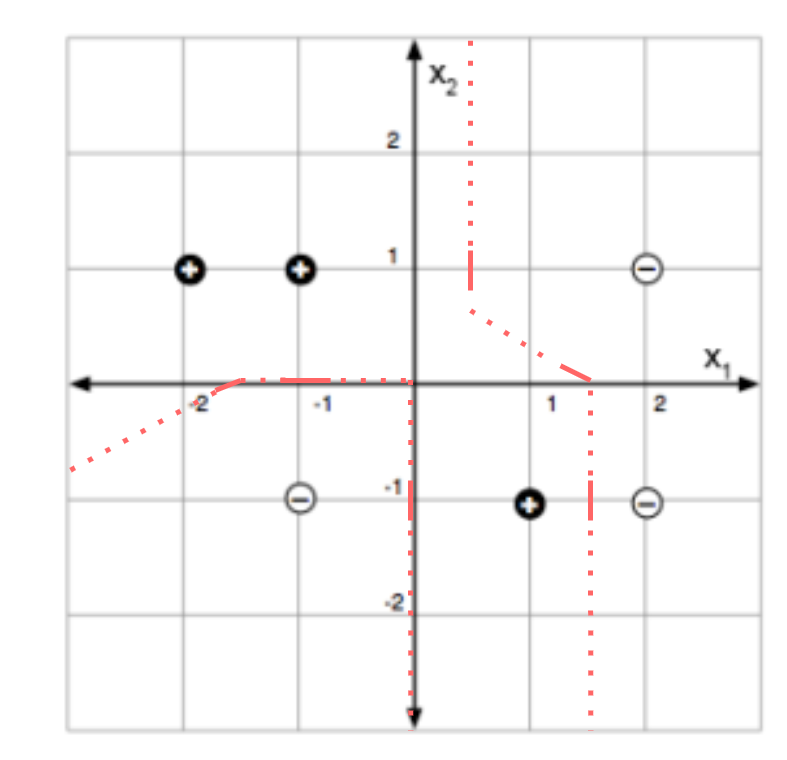
\includegraphics[width=40mm,scale=0.5]{images/nonparametric_images/lines_partly_drawn.png}
            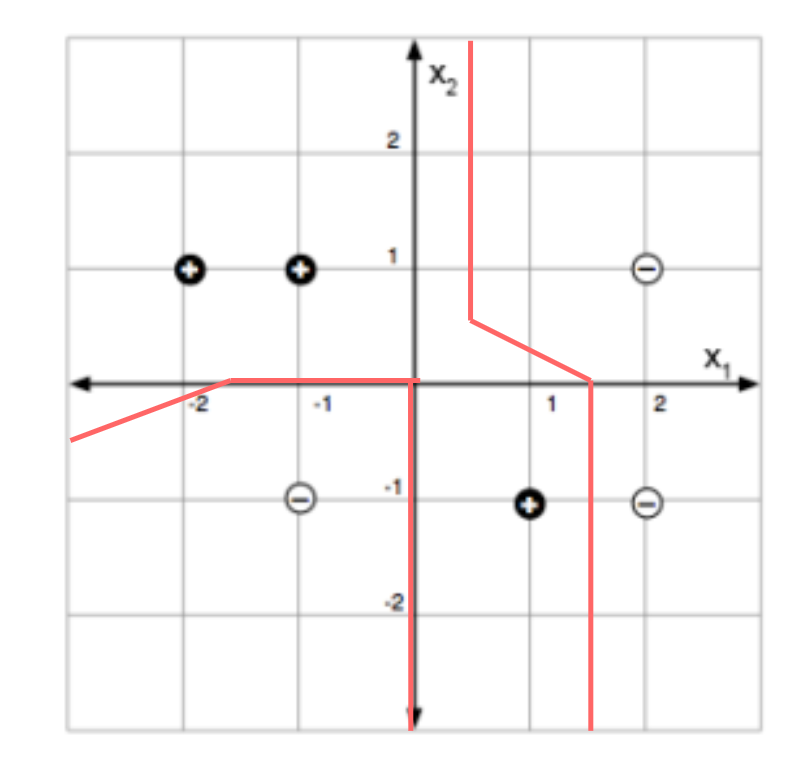
\includegraphics[width=40mm,scale=0.5]{images/nonparametric_images/lines_drawn.png}
    
            \caption*{We just have to draw our perpendiculars, and extend them.}
        \end{figure}

        The resulting diagram is a simplification of a \vocab{Voronoi diagram}.\\

        \begin{clarification}
            This system is for \redd{nearest neighbors}.

            You \redd{CANNOT} use it for \purp{$k$ nearest neighbors} (discussed below).
        \end{clarification}

            \note{If you try to use it this way, I will be sad.}

        Why is this a "simplified" voronoi diagram?

        \begin{itemize}
            \item In a real voronoi diagram, every single data point gets its own tile of "closer to this point than every other.

            \item In this one, we've simplified, so all of the $+$ and $-$ classifications join into one region.
        \end{itemize}

        \begin{figure}[H]
            \centering
            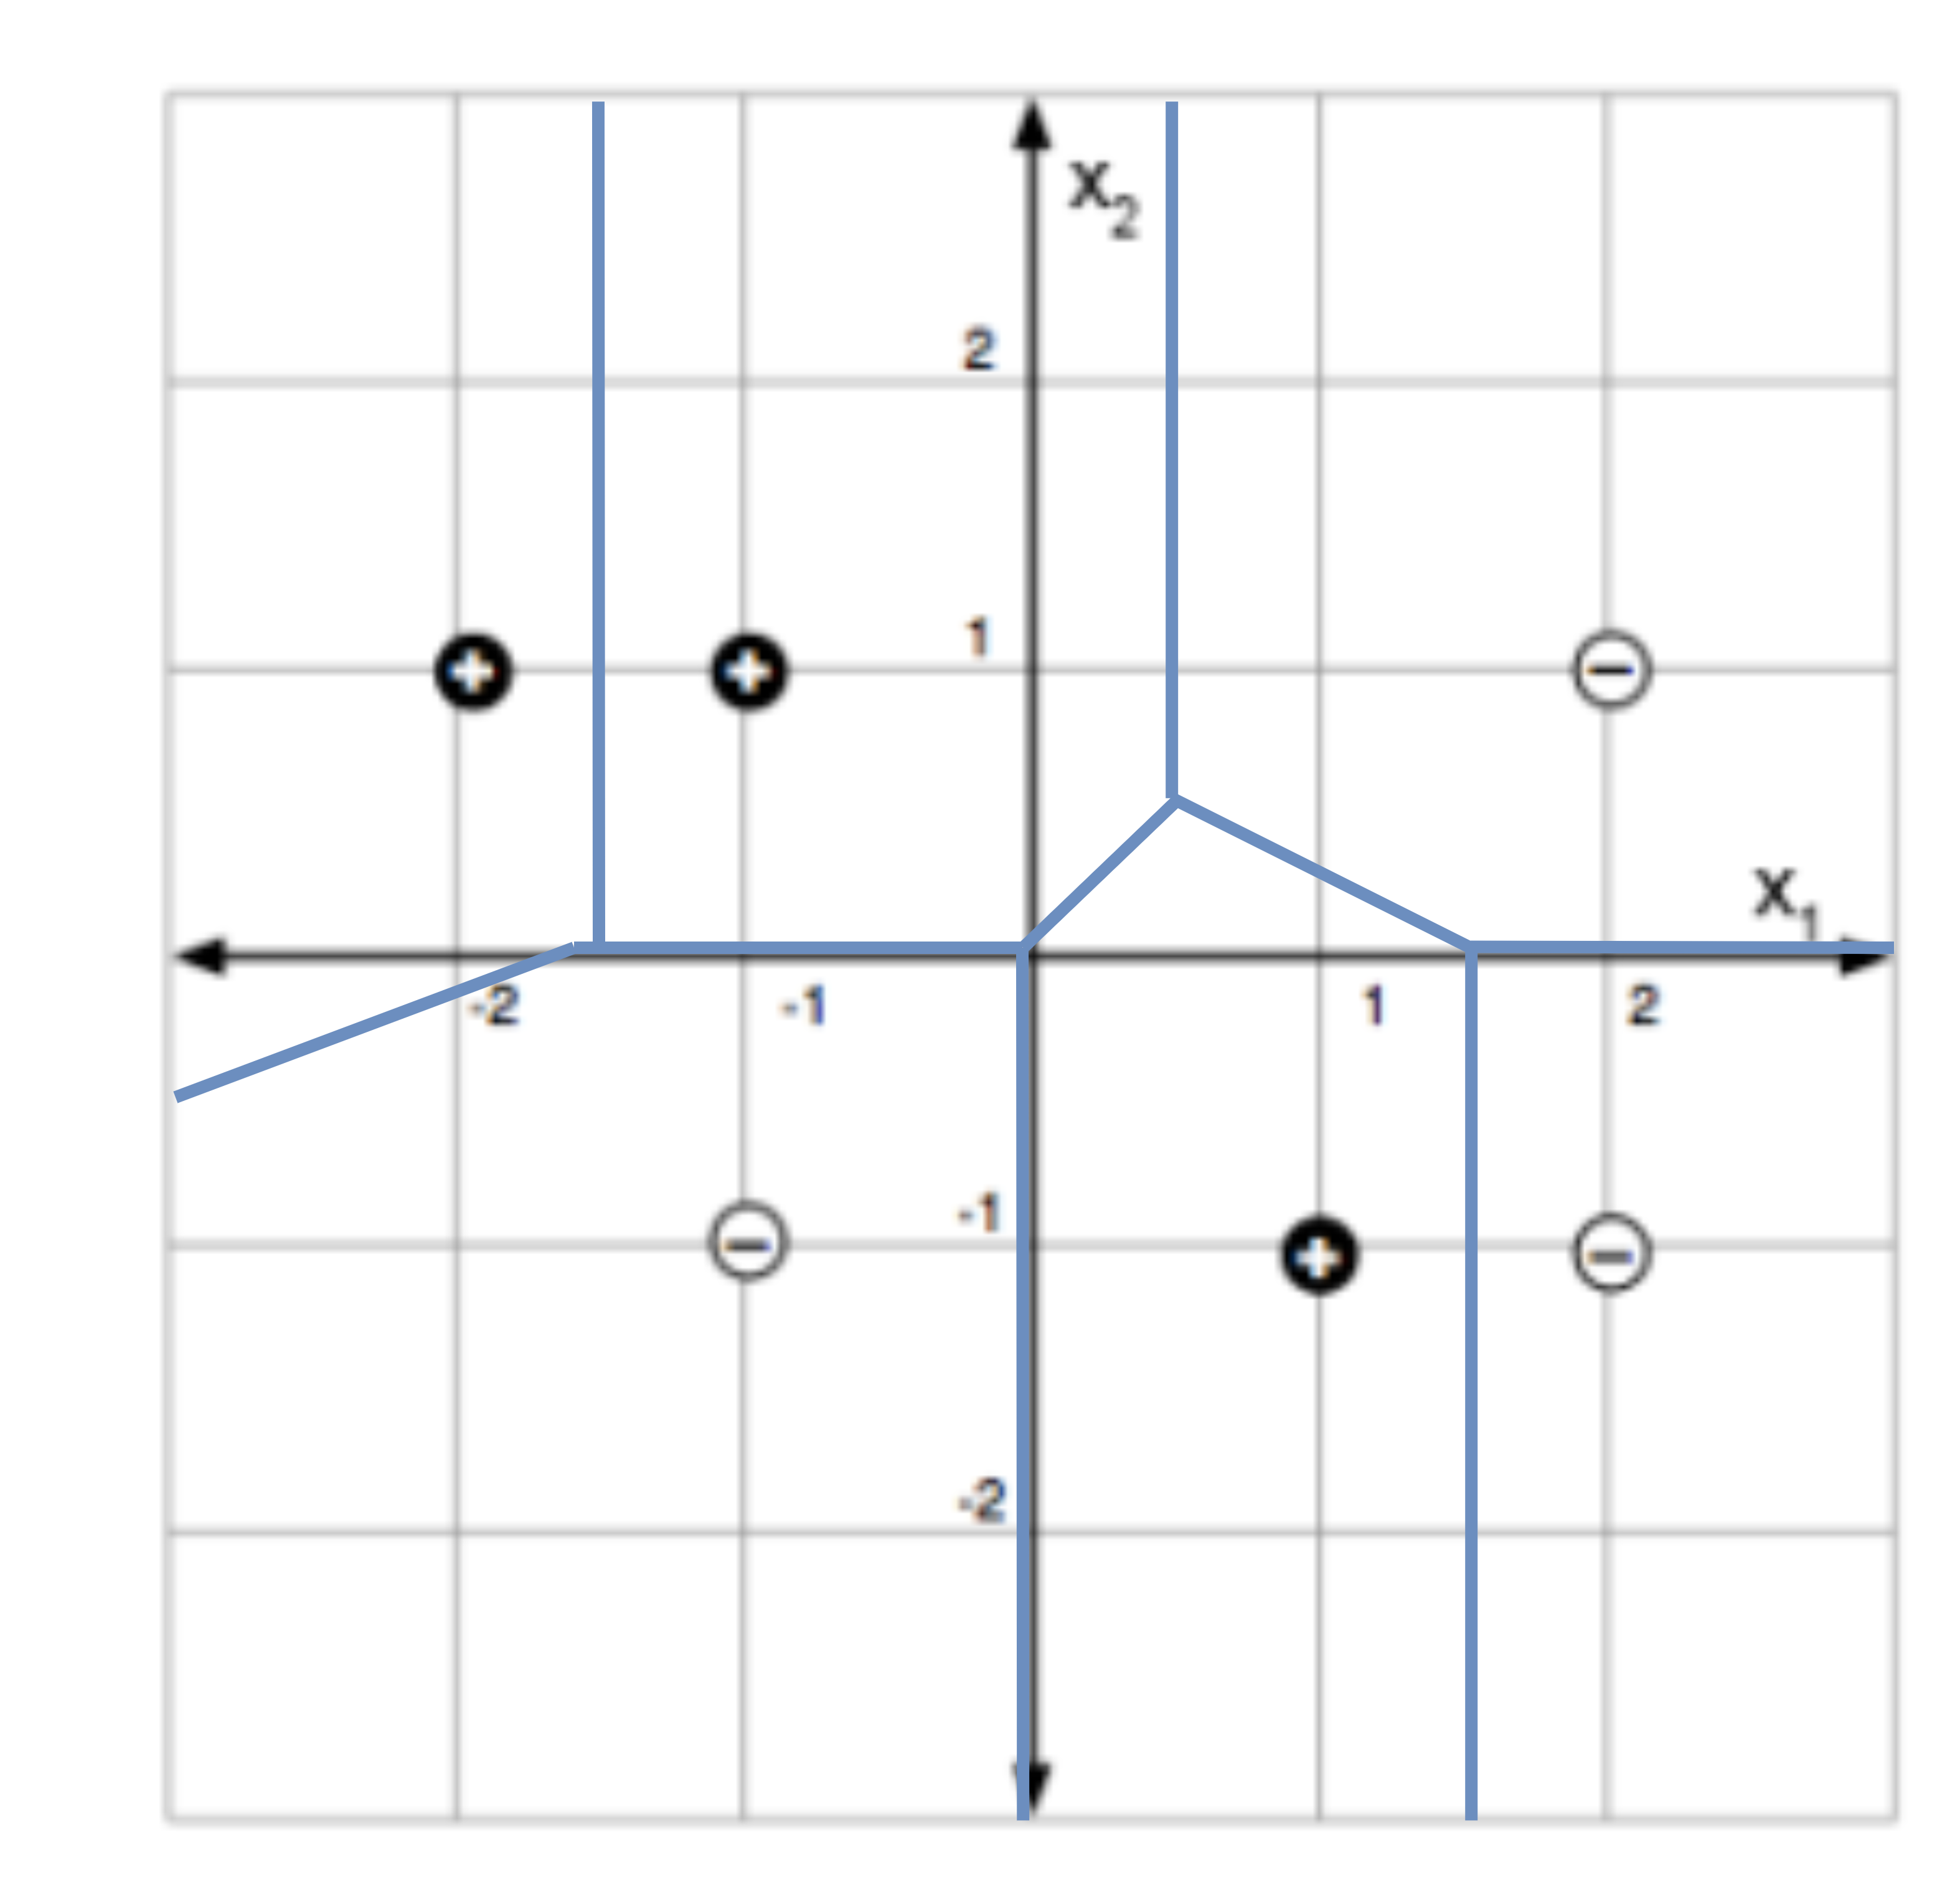
\includegraphics[width=60mm,scale=0.5]{images/nonparametric_images/voronoi_diagram.png}
    
            \caption*{Here's a "complete" voronoi diagram: each region represents all data which are closest to that particular data point.}
        \end{figure}
            
            



    \pagebreak
    

    \subsection{$k$-Nearest Neighbors}

        If one neighbor is too simplified, we can also use \purp{multiple} neighbors: our number of neighbors is $k$.\\
    
        \begin{definition}
            In the \vocab{$k$-nearest neighbors} (kNN), we use $k$ ($k \in \NN$) to give us the "size" of our neighborhood:
    
            \begin{itemize}
                \item When making a prediction, we only focus the $k$ nearest data points.
                \item We ignore all data points beyond the $\nth{k}$ one.
            \end{itemize}

            \subsecdiv
    
            This same approach can be applied to both \purp{regression} and \gren{classification}:
    
            \begin{itemize}
                \item In \purp{regression}, you would \orgg{average} the output of those $k$ nearest neighbors.
    
                \item In \gren{classification}, you would pick the \orgg{majority}: the most common label of your $k$ nearest neighbors.
            \end{itemize}
        \end{definition}
    
        \miniex Suppose your $k=4$ nearest neighbors had output values, $y = (3,4,5,6)$. You would predict your output by simply averaging them:
    
        \begin{equation}
            \frac{3+4+5+6}{4} = 4.5
        \end{equation}

        One reason to use $k$-nearest neighbors is that "nearest neighbor" ($k=1$) might \purp{overfit}.\\

        \begin{concept}
            Having a low $k$-value could be seen as \vocab{overfitting}:

            \begin{itemize}
                \item If you're closest to an \orgg{outlier} data point, you'll \purp{choose} that value, rather than the general trend you see with more data.
            \end{itemize}

            So, you're sensitive to \gren{noise} in the data, if you happen to be too close to that noise.

            \begin{itemize}
                \item With a larger $k$-value, you're \purp{averaging} over more data points: this can reduce the effect of noise.
            \end{itemize}
        \end{concept}

        In other words: you're not create a general pattern based on the data structure: you're closely matching the training data.

        \begin{figure}[H]
            \centering
            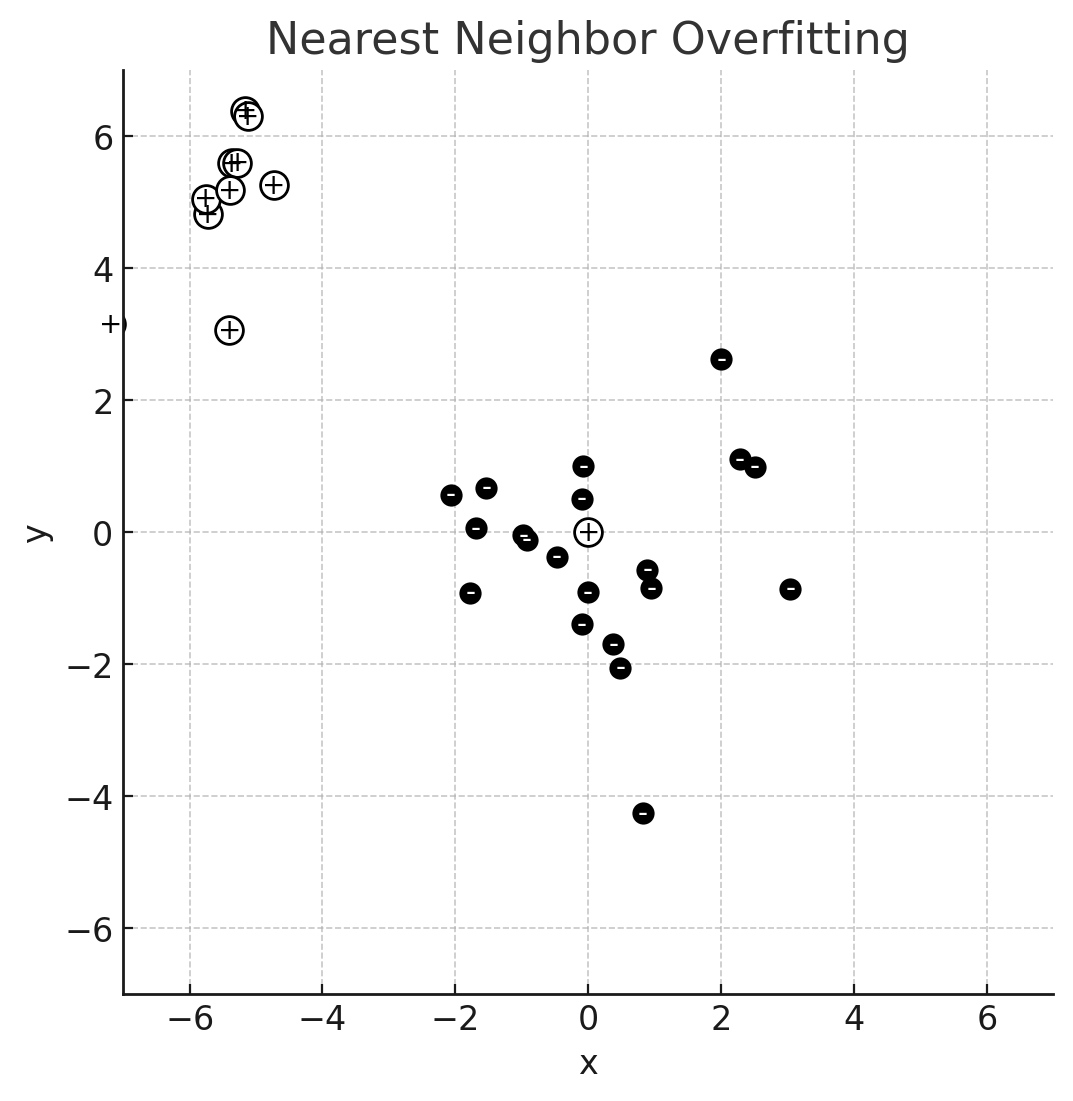
\includegraphics[width=50mm,scale=0.5]{images/nonparametric_images/nearest_neighbor_overfitting.png}
    
            \caption*{Suppose we happened to have a data point right next to (0,0). Based on the whole region, the result is probably a negative (-). But with $k=1$, we would assume it was positive.}
        \end{figure}

        What happens with different $k$-values? Here's a different dataset to test this out on:

        \begin{figure}[H]
            \centering
            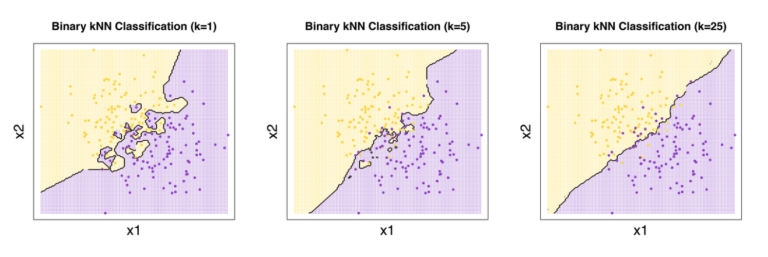
\includegraphics[width=140mm,scale=0.5]{images/nonparametric_images/knn_diff_k_values.png}
    
            \caption*{We can see that we get a more "general" pattern as $k$ increases. (Credit to \href{https://blog.eduonix.com/artificial-intelligence/k-nearest-neighbors-algorithm/}{blog.eduonix.com})}
        \end{figure}

        \begin{concept}
            On the opposite end, having a \vocab{high $k$-value} makes it more difficult to see more detailed trends, or fit well to \purp{complex} data.

            \begin{itemize}
                \item If the data really does have a complex shape, but our $k$ is \redd{too low}, we won't be able to match it.
            \end{itemize}

            In other words, we can "underfit" as well.
        \end{concept}

        \miniex In the extreme case: imagine that $k$ equals the size of our training data. That means, you always include \orgg{all of your training data} to make a judgement.

        \begin{itemize}
            \item No matter what input you give, you'll \purp{always} get the same output: the average of all data.
            \item That's not going to be very predictive.
        \end{itemize}

    \phantom{}

    \subsection{Locally weighted regression}

        Another technique is \textit{locally weighted regression}, where we use the local region to create a small regression model:\\

        \begin{definition}
            In \vocab{locally weighted regression}, we take the $k$ nearest data points, and \purp{fit} a regression model to only those data points. 

            We might \orgg{weigh} closer data points more heavily than those which are further away:

            \begin{itemize}
                \item Meaning, they're more important to the fitting process.
            \end{itemize}
        \end{definition}




    \phantom{}

    \subsection{Tradeoffs}

        One major concern for $k$-nearest neighbors is that it's a pain to compare a new data point to the \purp{entire training set}, to find the closest data points.

        \begin{itemize}
            \item So, it's important to use data structures (e.g., ball trees) that make it \purp{easier} to quickly find possible "nearest neighbors".
        \end{itemize}

        On the other hand, it's relatively easy to \orgg{interpret} nearest neighbors:

        \begin{itemize}
            \item If you want to know why you got the answer that you did, you can directly view your "\gren{nearest neighbors}": these exact data points gave you your answer.
            \item This makes it easier to check for strange \purp{outliers}, or interesting patterns.
        \end{itemize}
    
    \pagebreak

    \subsection{Distance metrics (\redd{Optional})}

        What do we mean when we say that two data points are "close" or "far away"? 

        \begin{itemize}
            \item This requires us to have some kind of way to measure \gren{distance}: a \vocab{distance metric}.

            \item Above, we were using the \purp{euclidean} distance metric.\\
        \end{itemize}

        \begin{definition}
            A \vocab{distance metric} $d$ is one way of measuring the total distance between two data points.

            It must follow three basic rules:

            \begin{itemize}
                \item The distance from $x$ to \orgg{itself} is 0.

                \begin{equation*}
                    d(x,x) = 0
                \end{equation*}

                \item Distance is always \purp{positive}.

                \begin{equation*}
                    d(a,b)>0
                \end{equation*}

                \item The distance from $a$ to $b$ is the \gren{same} as the distance from $b$ to $a$.

                \begin{equation*}
                    d(a,b)=d(b,a)
                \end{equation*}

                \item \vocab{Triangle Inequality}: A \purp{direct path} from $a$ to $c$ is always the \gren{shortest} -- taking a detour from $a$ to $b$ cannot be faster.

                \begin{equation*}
                    d(a,c) \leq d(a,b) + d(b,c)
                \end{equation*}
            \end{itemize}

            
        \end{definition}

        Different metrics may be useful for different situations, or different data types.

        Here's a few common distance metrics:

        \begin{itemize}
            \item \vocab{Euclidean} distance: the "shortest path" distance in space.

                \begin{equation}
                    d(a,b) = \sqrt{\sum_i (a_i-b_i)^2}
                \end{equation}

                \begin{figure}[H]
                    \centering
                    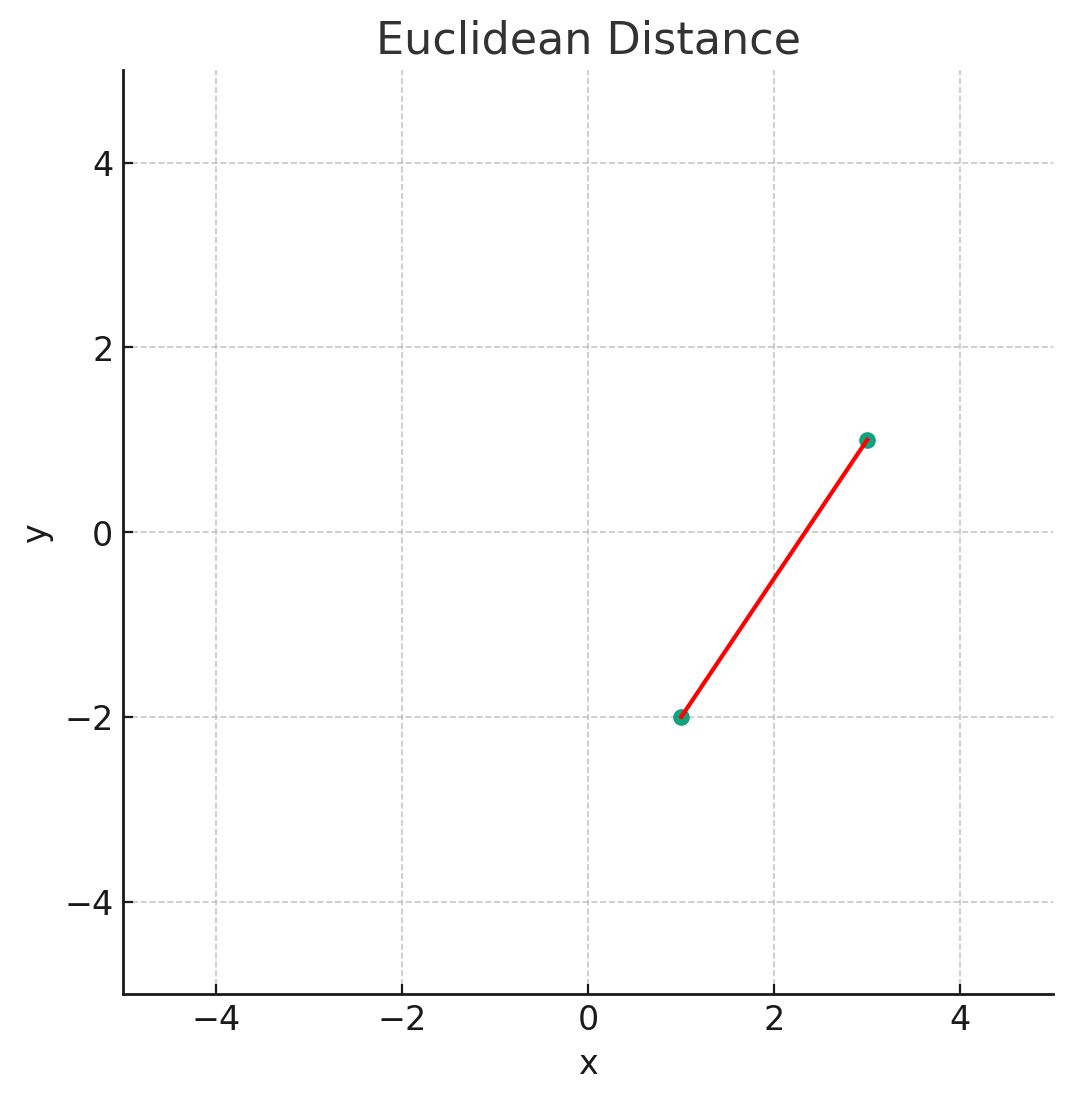
\includegraphics[width=40mm,scale=0.5]{images/nonparametric_images/euclidean_distance.png}
                    \caption*{Here, we have $\sqrt{(3-1)^2+(1-(-2))^2}=\sqrt{13}$}
                \end{figure}
                
            \item \vocab{Manhattan} distance: the "shortest path", while only moving along one axis at a time.

                \begin{equation}
                    d(a,b) = \sum_i \Big(\big| a_i-b_i \big| \Big)
                \end{equation}

                \begin{figure}[H]
                    \centering
                    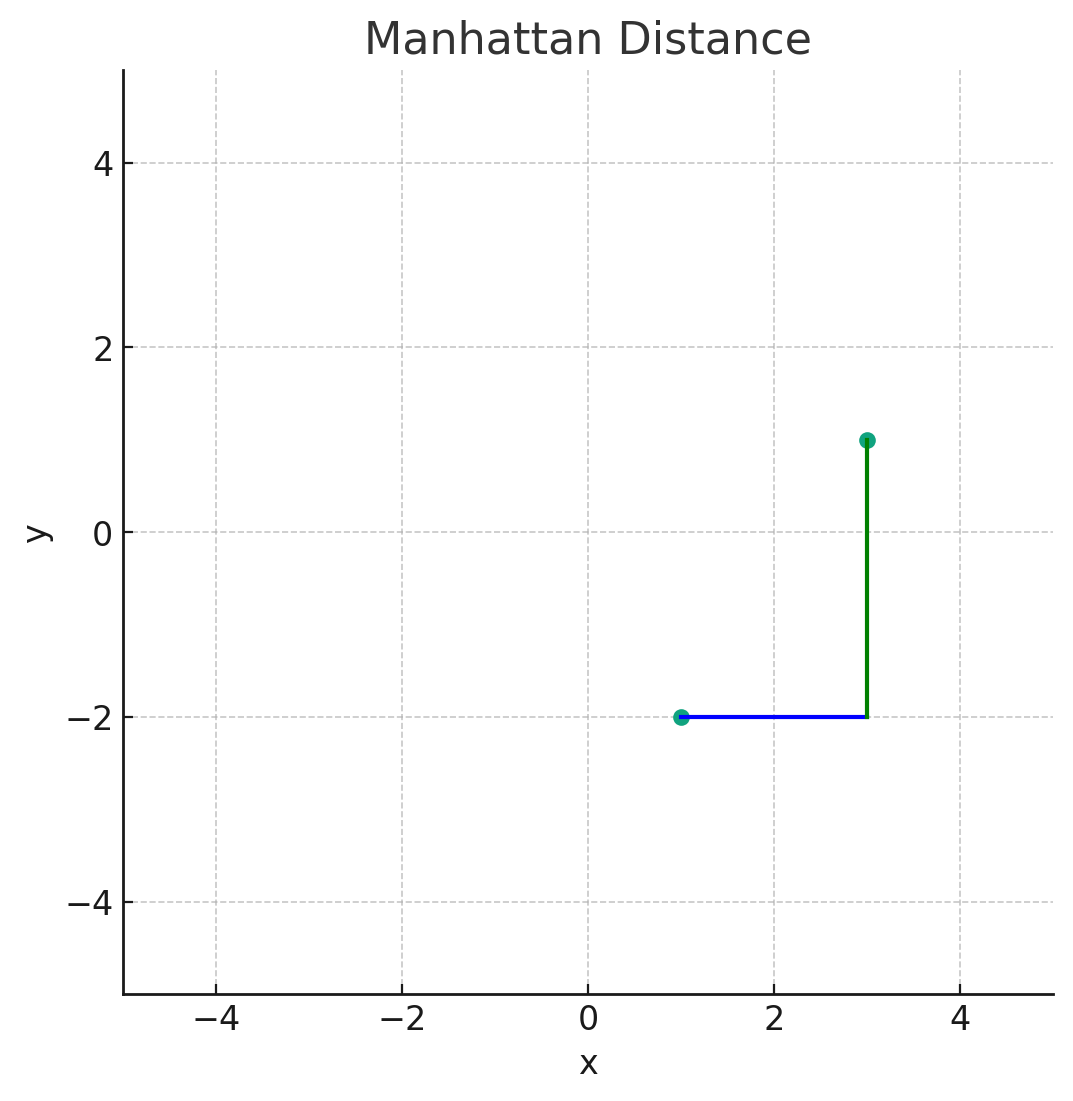
\includegraphics[width=40mm,scale=0.5]{images/nonparametric_images/manhattan_distance.png}
                    \caption*{Here, we have $|3-1|+|1-(-2)|=5$}
                \end{figure}
                

            \item \vocab{Hamming distance}: if we have two binary codes, how many digits are different between them?

                \begin{equation}
                    d(a,b) = \sum_i \Big( \mathbb{1} \big( a_i \neq b_i) \Big)
                \end{equation}

                \begin{equation}
                    a = \begin{bmatrix}
                        1 \\ \blu{0} \\ 0 \\ \blu{1} \\ 1 
                    \end{bmatrix}
                    \quad
                    b = \begin{bmatrix}
                        1 \\ \red{1} \\ 0 \\ \red{0} \\ 1 
                    \end{bmatrix}
                    \qquad\implies\qquad 
                    d(a,b)=2
                \end{equation}
        \end{itemize}

        And as a bonus:

        \begin{itemize}
            \item \vocab{Minkowsky} distance: a generalized version of the euclidean/manhattan distance: 
                \note{Notice that, for $p=1$, it's equal to manhattan. For $p=2$, it's equal to euclidean.}

                \begin{equation}
                    d(a,b) = \Big( \sum_i (a_i-b_i)^p \Big)^{1/p}
                \end{equation}
        \end{itemize}


    


        










\pagebreak


\section{Tree Models}

    Here, we'll create another algorithm, based on a common way that humans solve problems.

    \begin{itemize}
        \item You might ask a series of \purp{questions}, to narrow your situation down to a more specific example, that you know how to solve.
    \end{itemize}

    \begin{figure}[H]
        \centering
        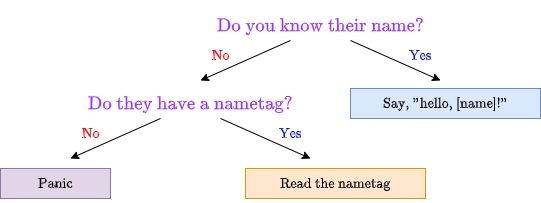
\includegraphics[width=70mm,scale=0.5]{images/nonparametric_images/tree_simple.png}
        \caption*{This tree answers the question, "how to start a conversation?". Panicking may not be the optimal strategy, but it's what this tree advises.}
    \end{figure}

    Each question is simple: a \gren{binary}, "yes or no" question. But with enough questions, you can get pretty specific classifications:

    \begin{figure}[H]
        \centering
        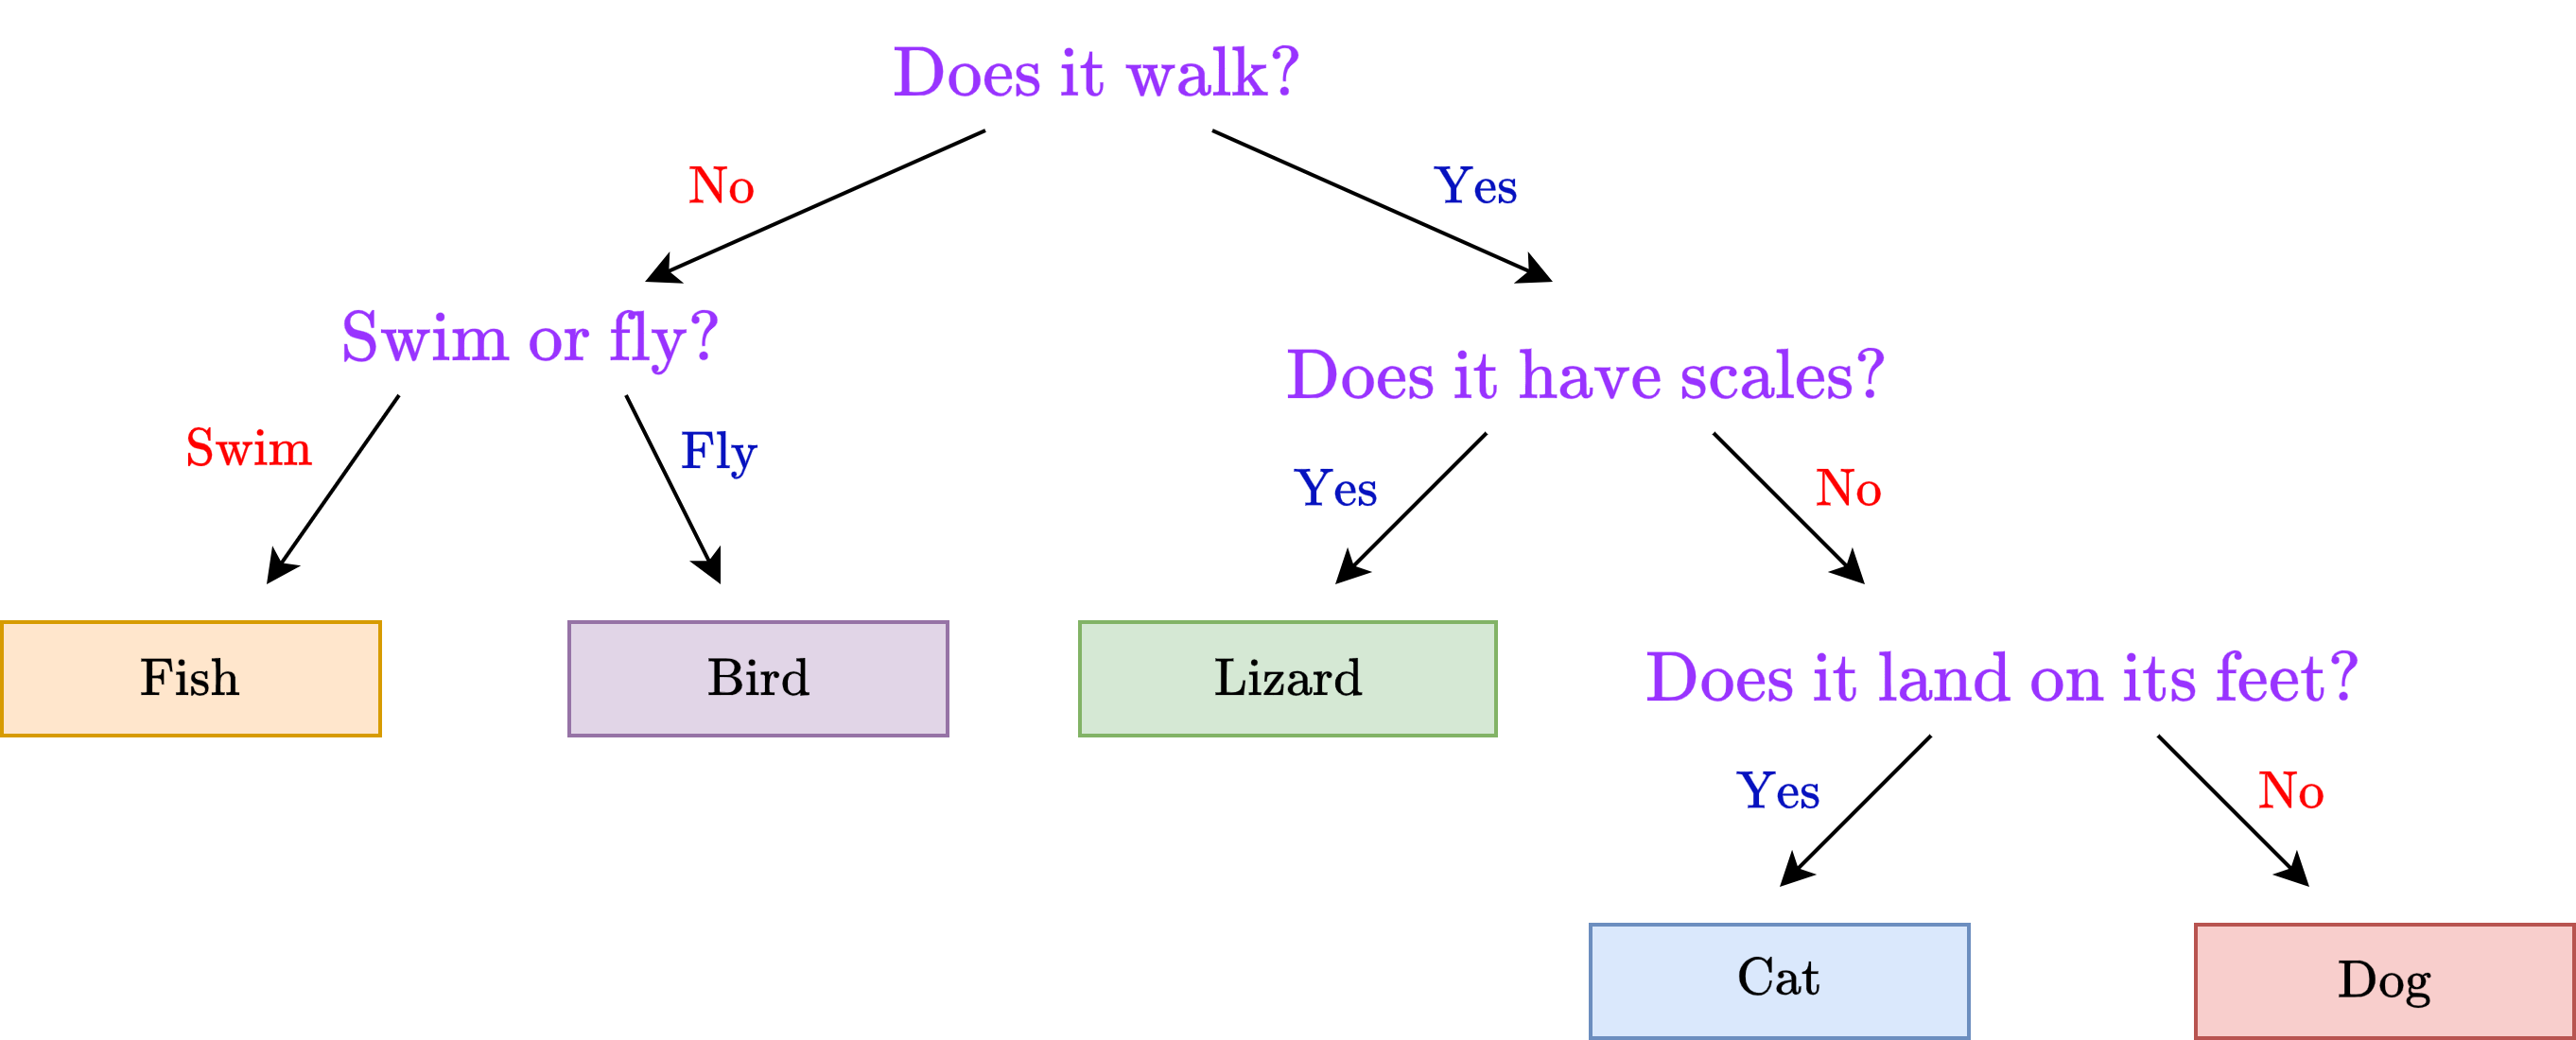
\includegraphics[width=90mm,scale=0.5]{images/nonparametric_images/tree_complex.png}
        \caption*{A tree for classifying household pets. A bit too simple to be fully accurate.}
    \end{figure}

    \begin{definition}
        A \vocab{binary tree} is a structure where:

        \begin{itemize}
            \item You start at a \vocab{root node}: the \purp{top} of the tree.
            
            \item At each node, you \orgg{split} your data into two "branches", based on a \gren{binary} (yes-or-no) question.

            \item You \purp{terminate} at a \vocab{leaf node}: each leaf node stops branching, and returns an output $y$.
            
        \end{itemize}
    \end{definition}

    The above diagrams show a strength of tree diagrams: they are \orgg{very interpretable}.\\

    \begin{concept}
        \vocab{Tree models} tend to be more interpretable than most other types of models.
    \end{concept}

    They're so interpretable, that they can even be used for day-to-day problems, like medical analysis:

    \begin{figure}[H]
        \centering
        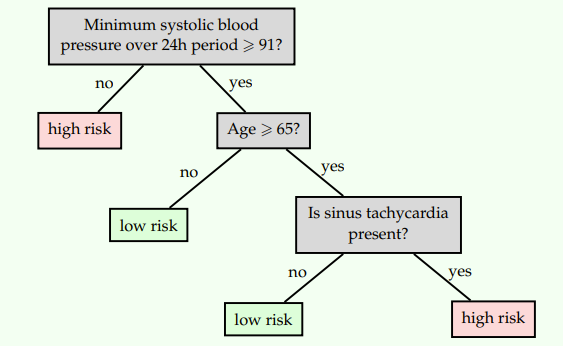
\includegraphics[width=70mm,scale=0.5]{images/nonparametric_images/medical_tree.png}
        \caption*{Reproduced from Breiman, Friedman, Olshen, Stone (1984).}
    \end{figure}

    However, they tend to work best on data with a small number of input dimensions, or at least a small number that matter.\\

    \begin{concept}
        \vocab{Tree models} tend to work best on datasets with:

        \begin{itemize}
            \item Low dimensionality
            \item A small number of individual dimensions contain a lot of information
        \end{itemize}
    \end{concept}

    Otherwise, it can take a huge number of splits to get a productive result.





    


    \pagebreak

    \subsection{An example in 2D space}

        The examples we've shown so far have all been abstract, categorical questions. Now, let's consider an example where we have a \purp{continuous} input space, 2D space.

        We'll re-use the plot from the nearest-neighbor section:

        \begin{figure}[H]
            \centering
            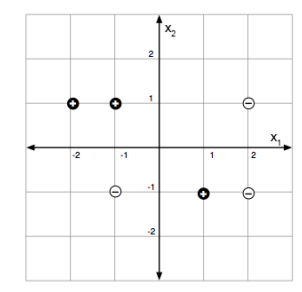
\includegraphics[width=50mm,scale=0.5]{images/nonparametric_images/classification_example.png}

            \caption*{Our goal is to split the space up, so that we can classify more easily.}
        \end{figure}

        This is the type of problem we'll deal with for the rest of the chapter: \vocab{$n$-dimensional, real-valued} space.

        How do we want to split up our space? For simplicity, we'll only use \gren{one axis} for each split.\\

        \begin{definition}
            Our \vocab{tree-generating algorithm} will split the data along \orgg{one axis at a time}:

            \begin{equation*}
                x_i \geq C \qquad \text{ or } \qquad x_i < C
            \end{equation*}
            
        \end{definition}

         Let's give an example: what split would help you classify data?
         
         \begin{itemize}
             \item The two rightmost data points are both \orgg{negative}. So, let's separate them from the rest of the data:
         \end{itemize}

         \begin{equation}
             x_1 \geq 1.5
         \end{equation}

         \begin{figure}[H]
            \centering
            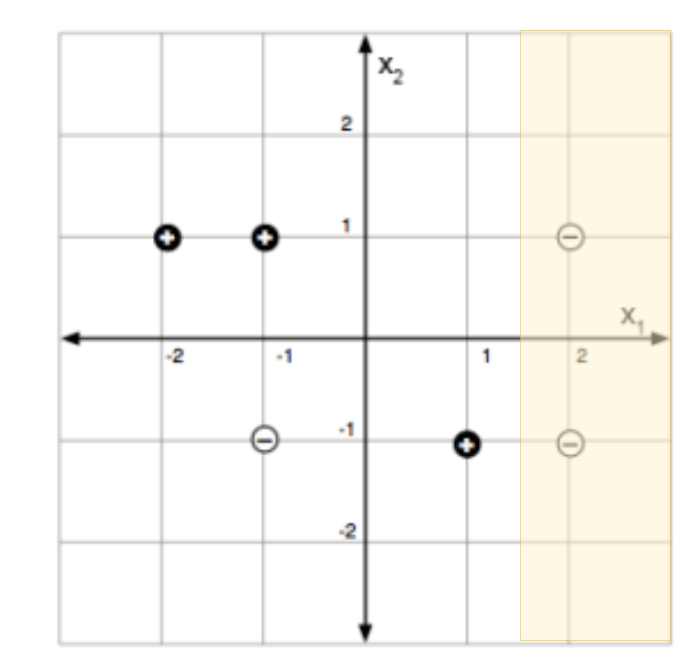
\includegraphics[width=50mm,scale=0.5]{images/nonparametric_images/x1_geq_1_5.png}
            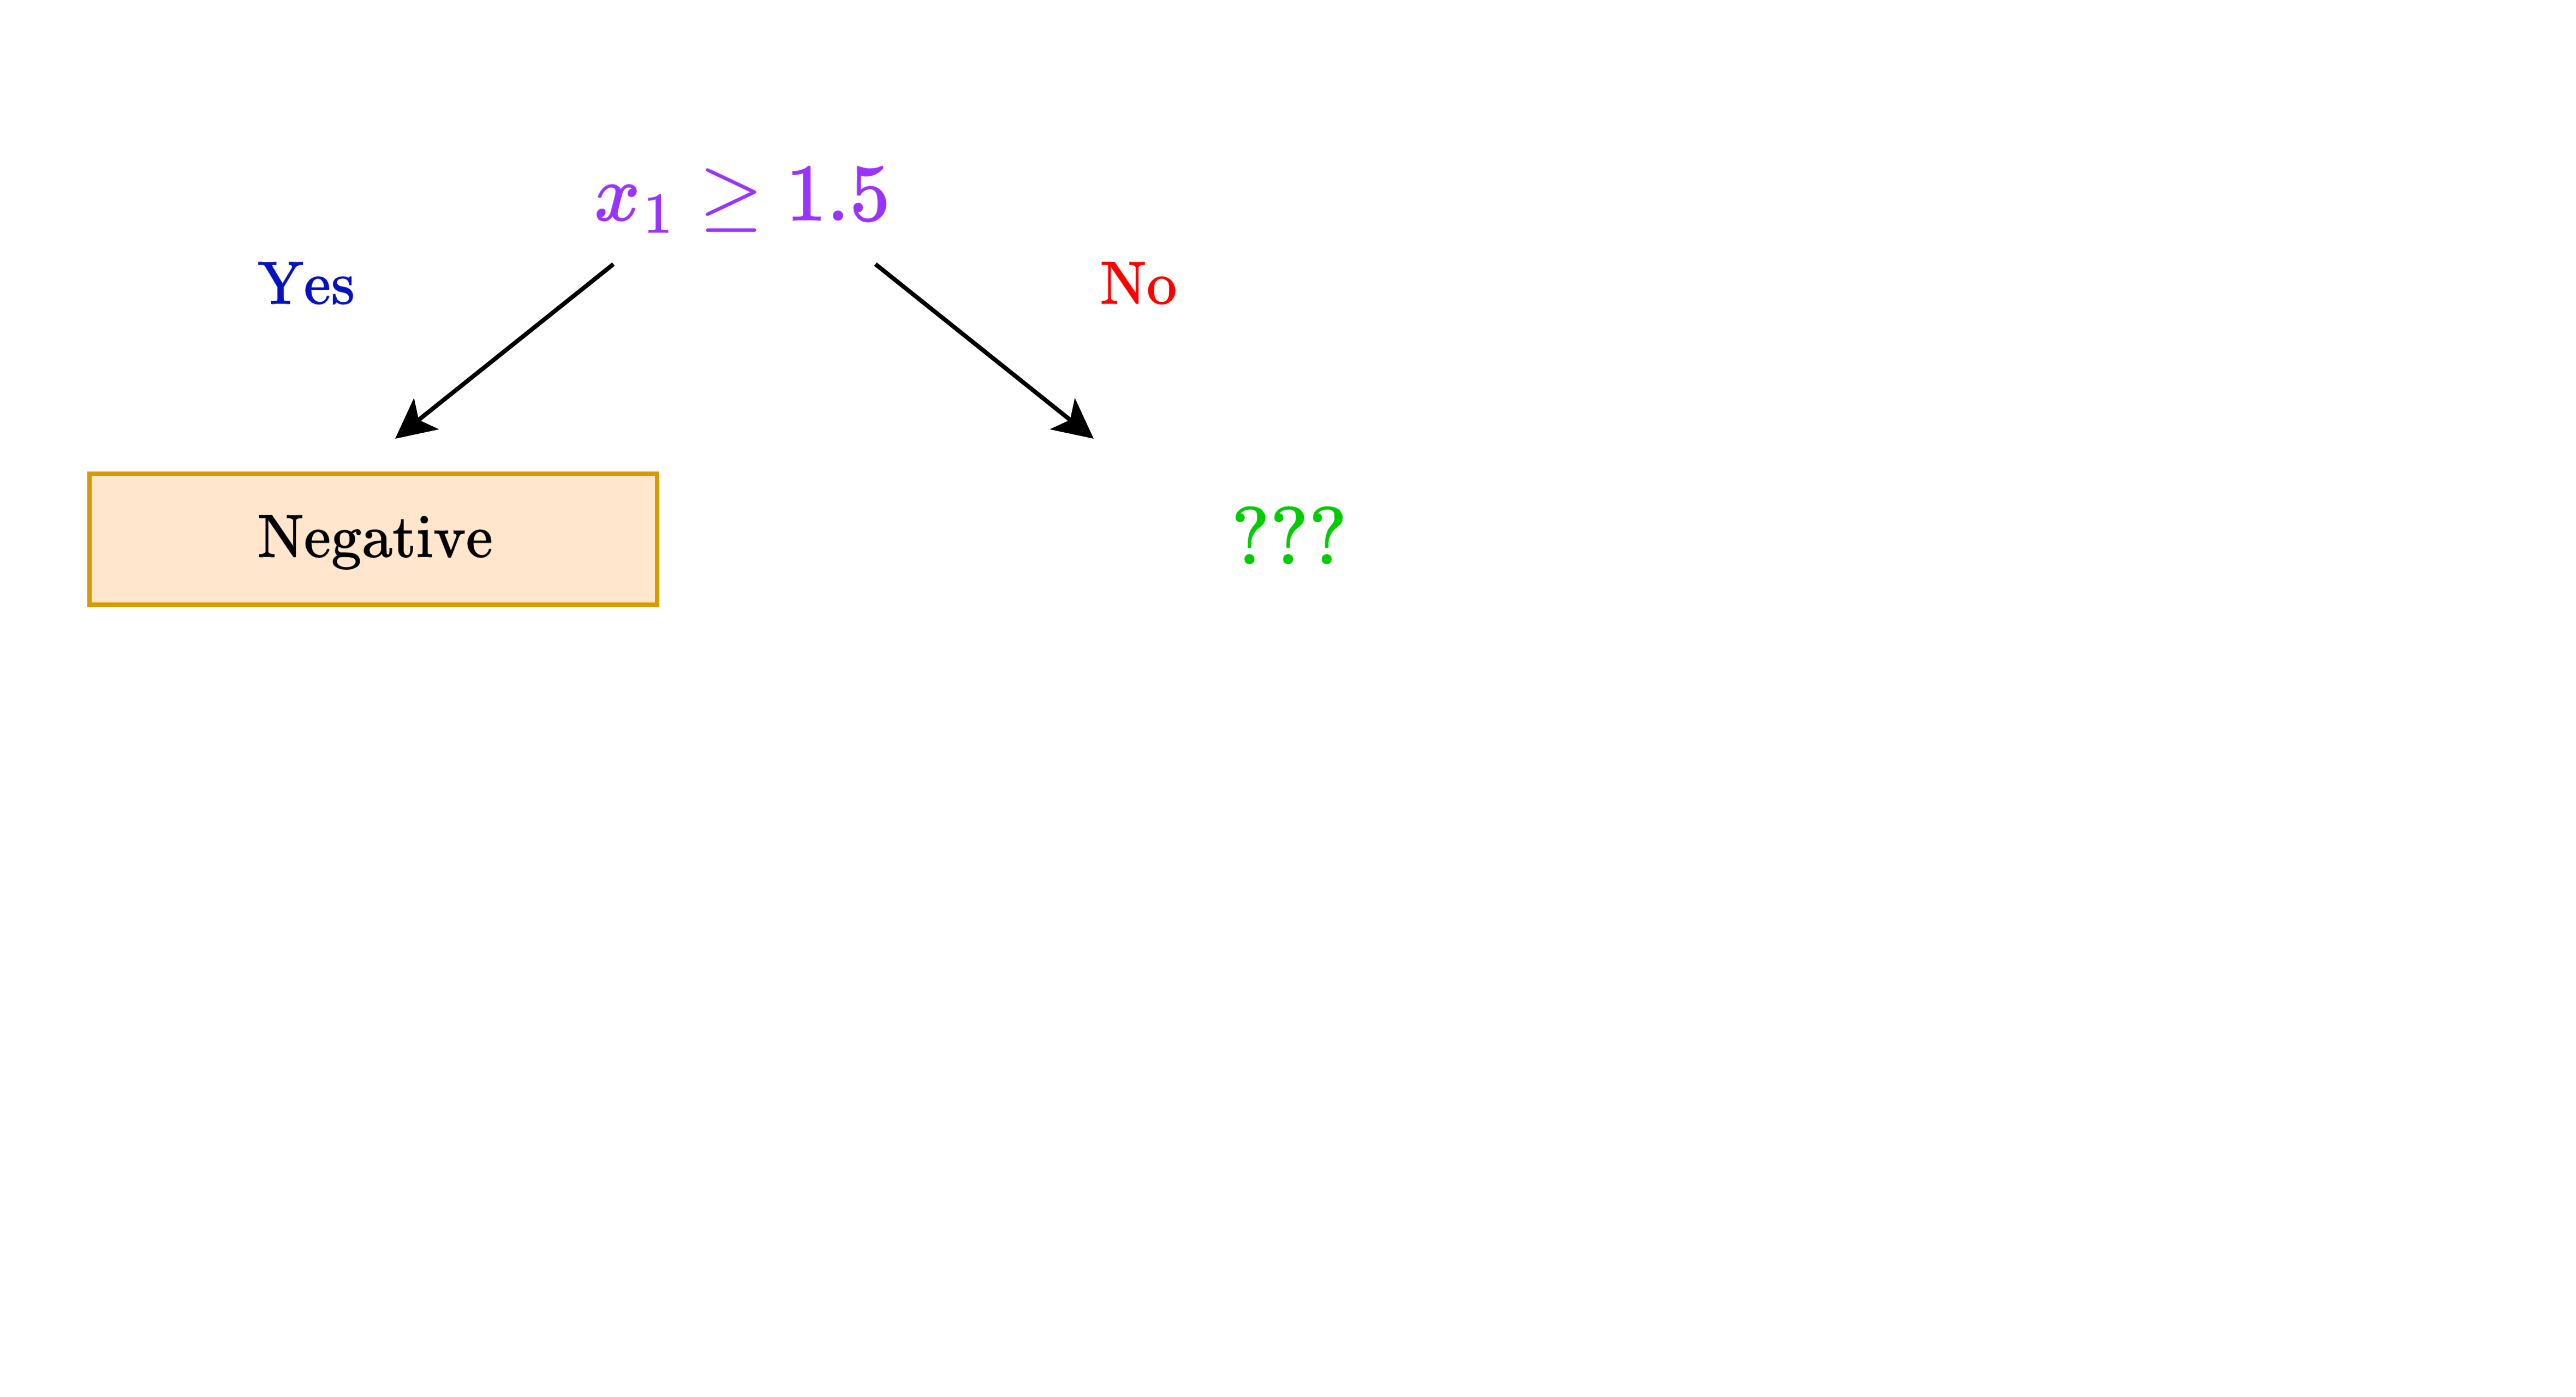
\includegraphics[width=85mm,scale=0.5]{images/nonparametric_images/x1_geq_1_5_tree.png}
            \caption*{We've split our dataset once.}
        \end{figure}

        The right side is taken care of: everything is \orgg{negative}. Let's take our first attempt at splitting the left side.

        \begin{itemize}
            \item The top two data points are both \gren{positive}.
        \end{itemize}

        \begin{equation}
             x_2 \geq 0
         \end{equation}

         \begin{figure}[H]
            \centering
            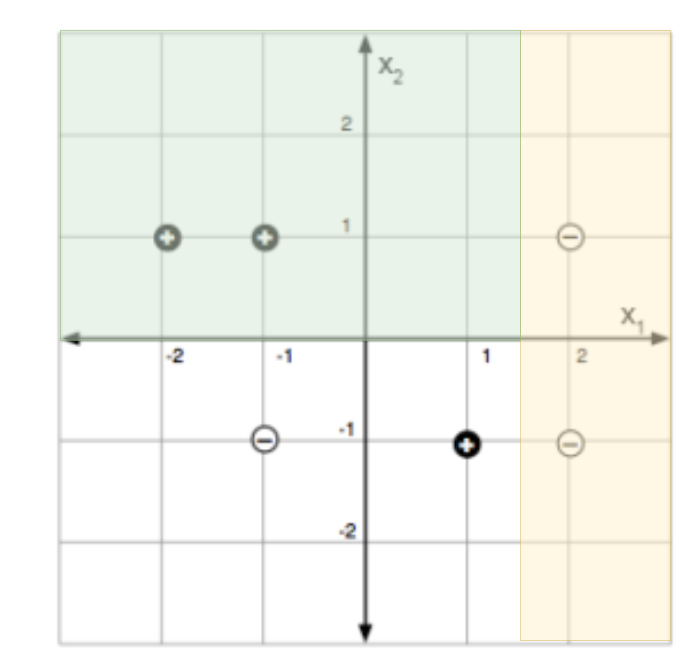
\includegraphics[width=50mm,scale=0.5]{images/nonparametric_images/x2_geq_0.png}
            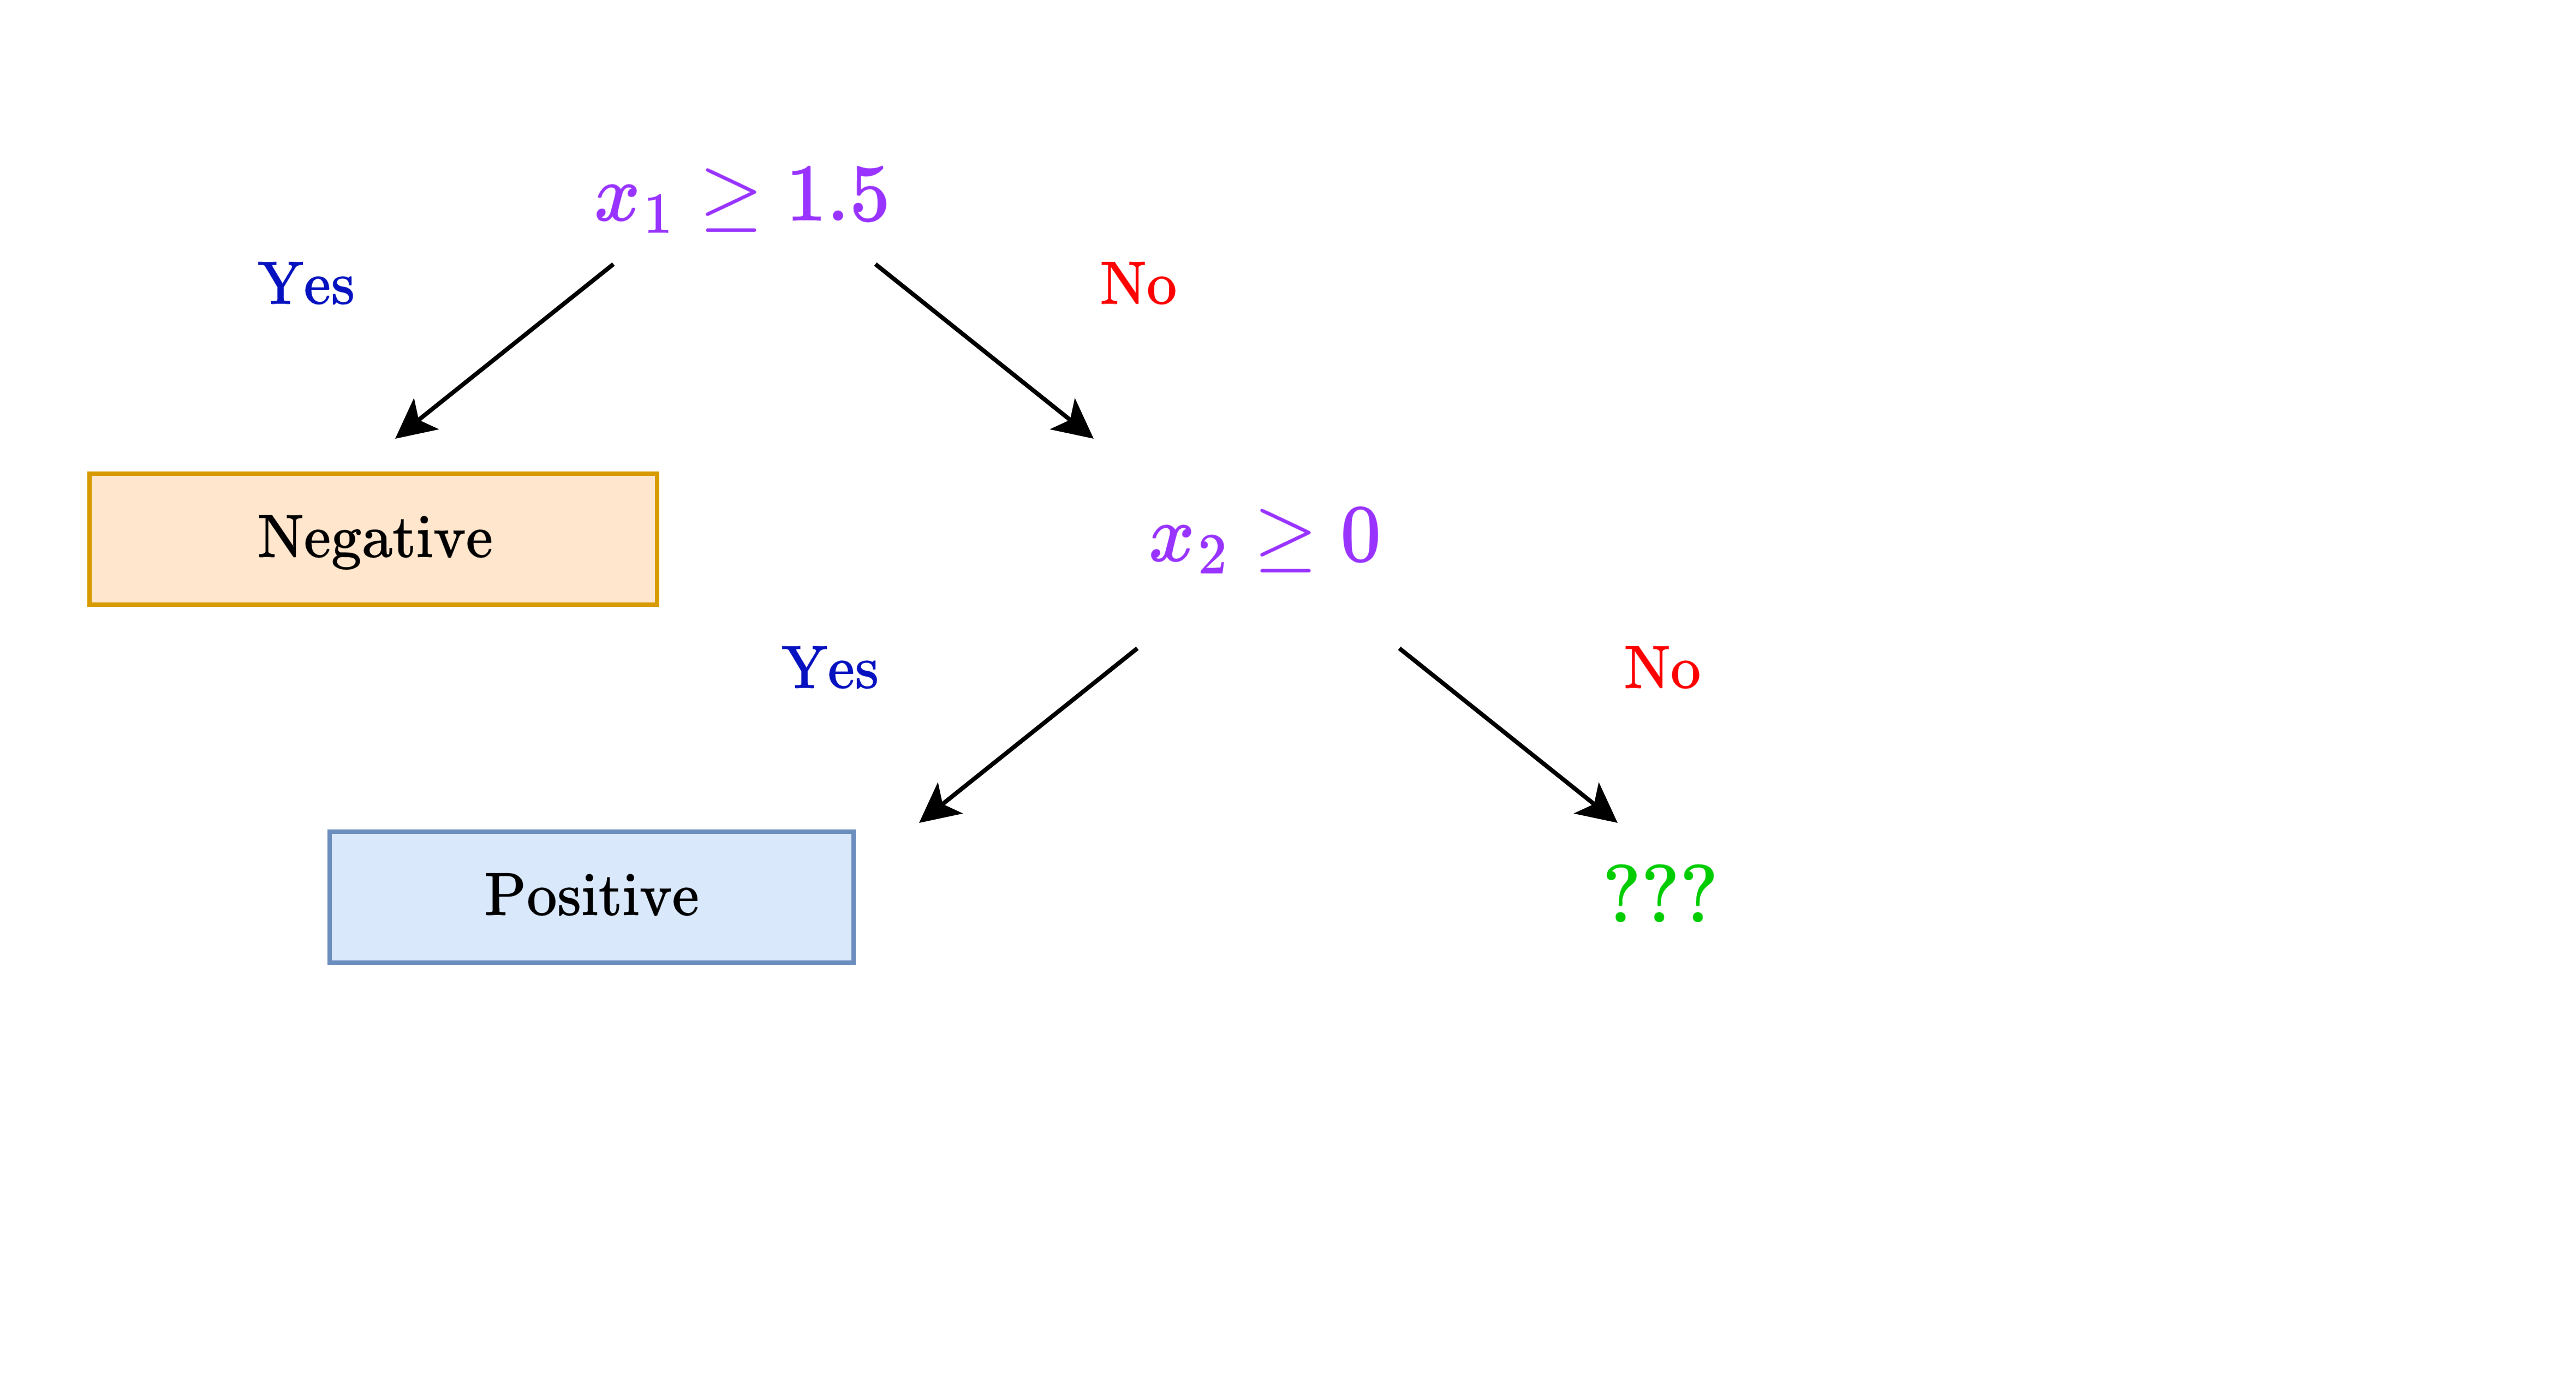
\includegraphics[width=85mm,scale=0.5]{images/nonparametric_images/x2_geq_0_tree.png}
            \caption*{Another split.}
        \end{figure}

        We only have to make one more split: between the positive and negative data point.

        \begin{equation}
            x_1\geq 0
        \end{equation}
        
        \begin{figure}[H]
            \centering
            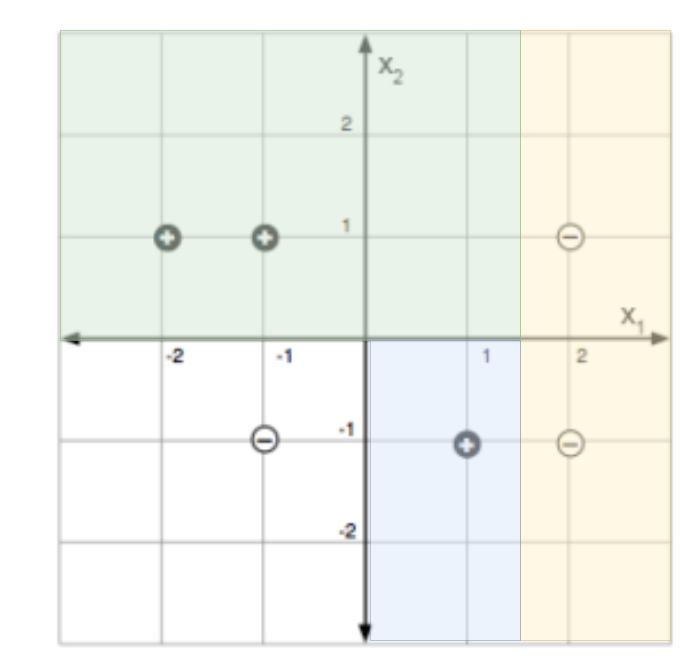
\includegraphics[width=50mm,scale=0.5]{images/nonparametric_images/x1_geq_0.png}
            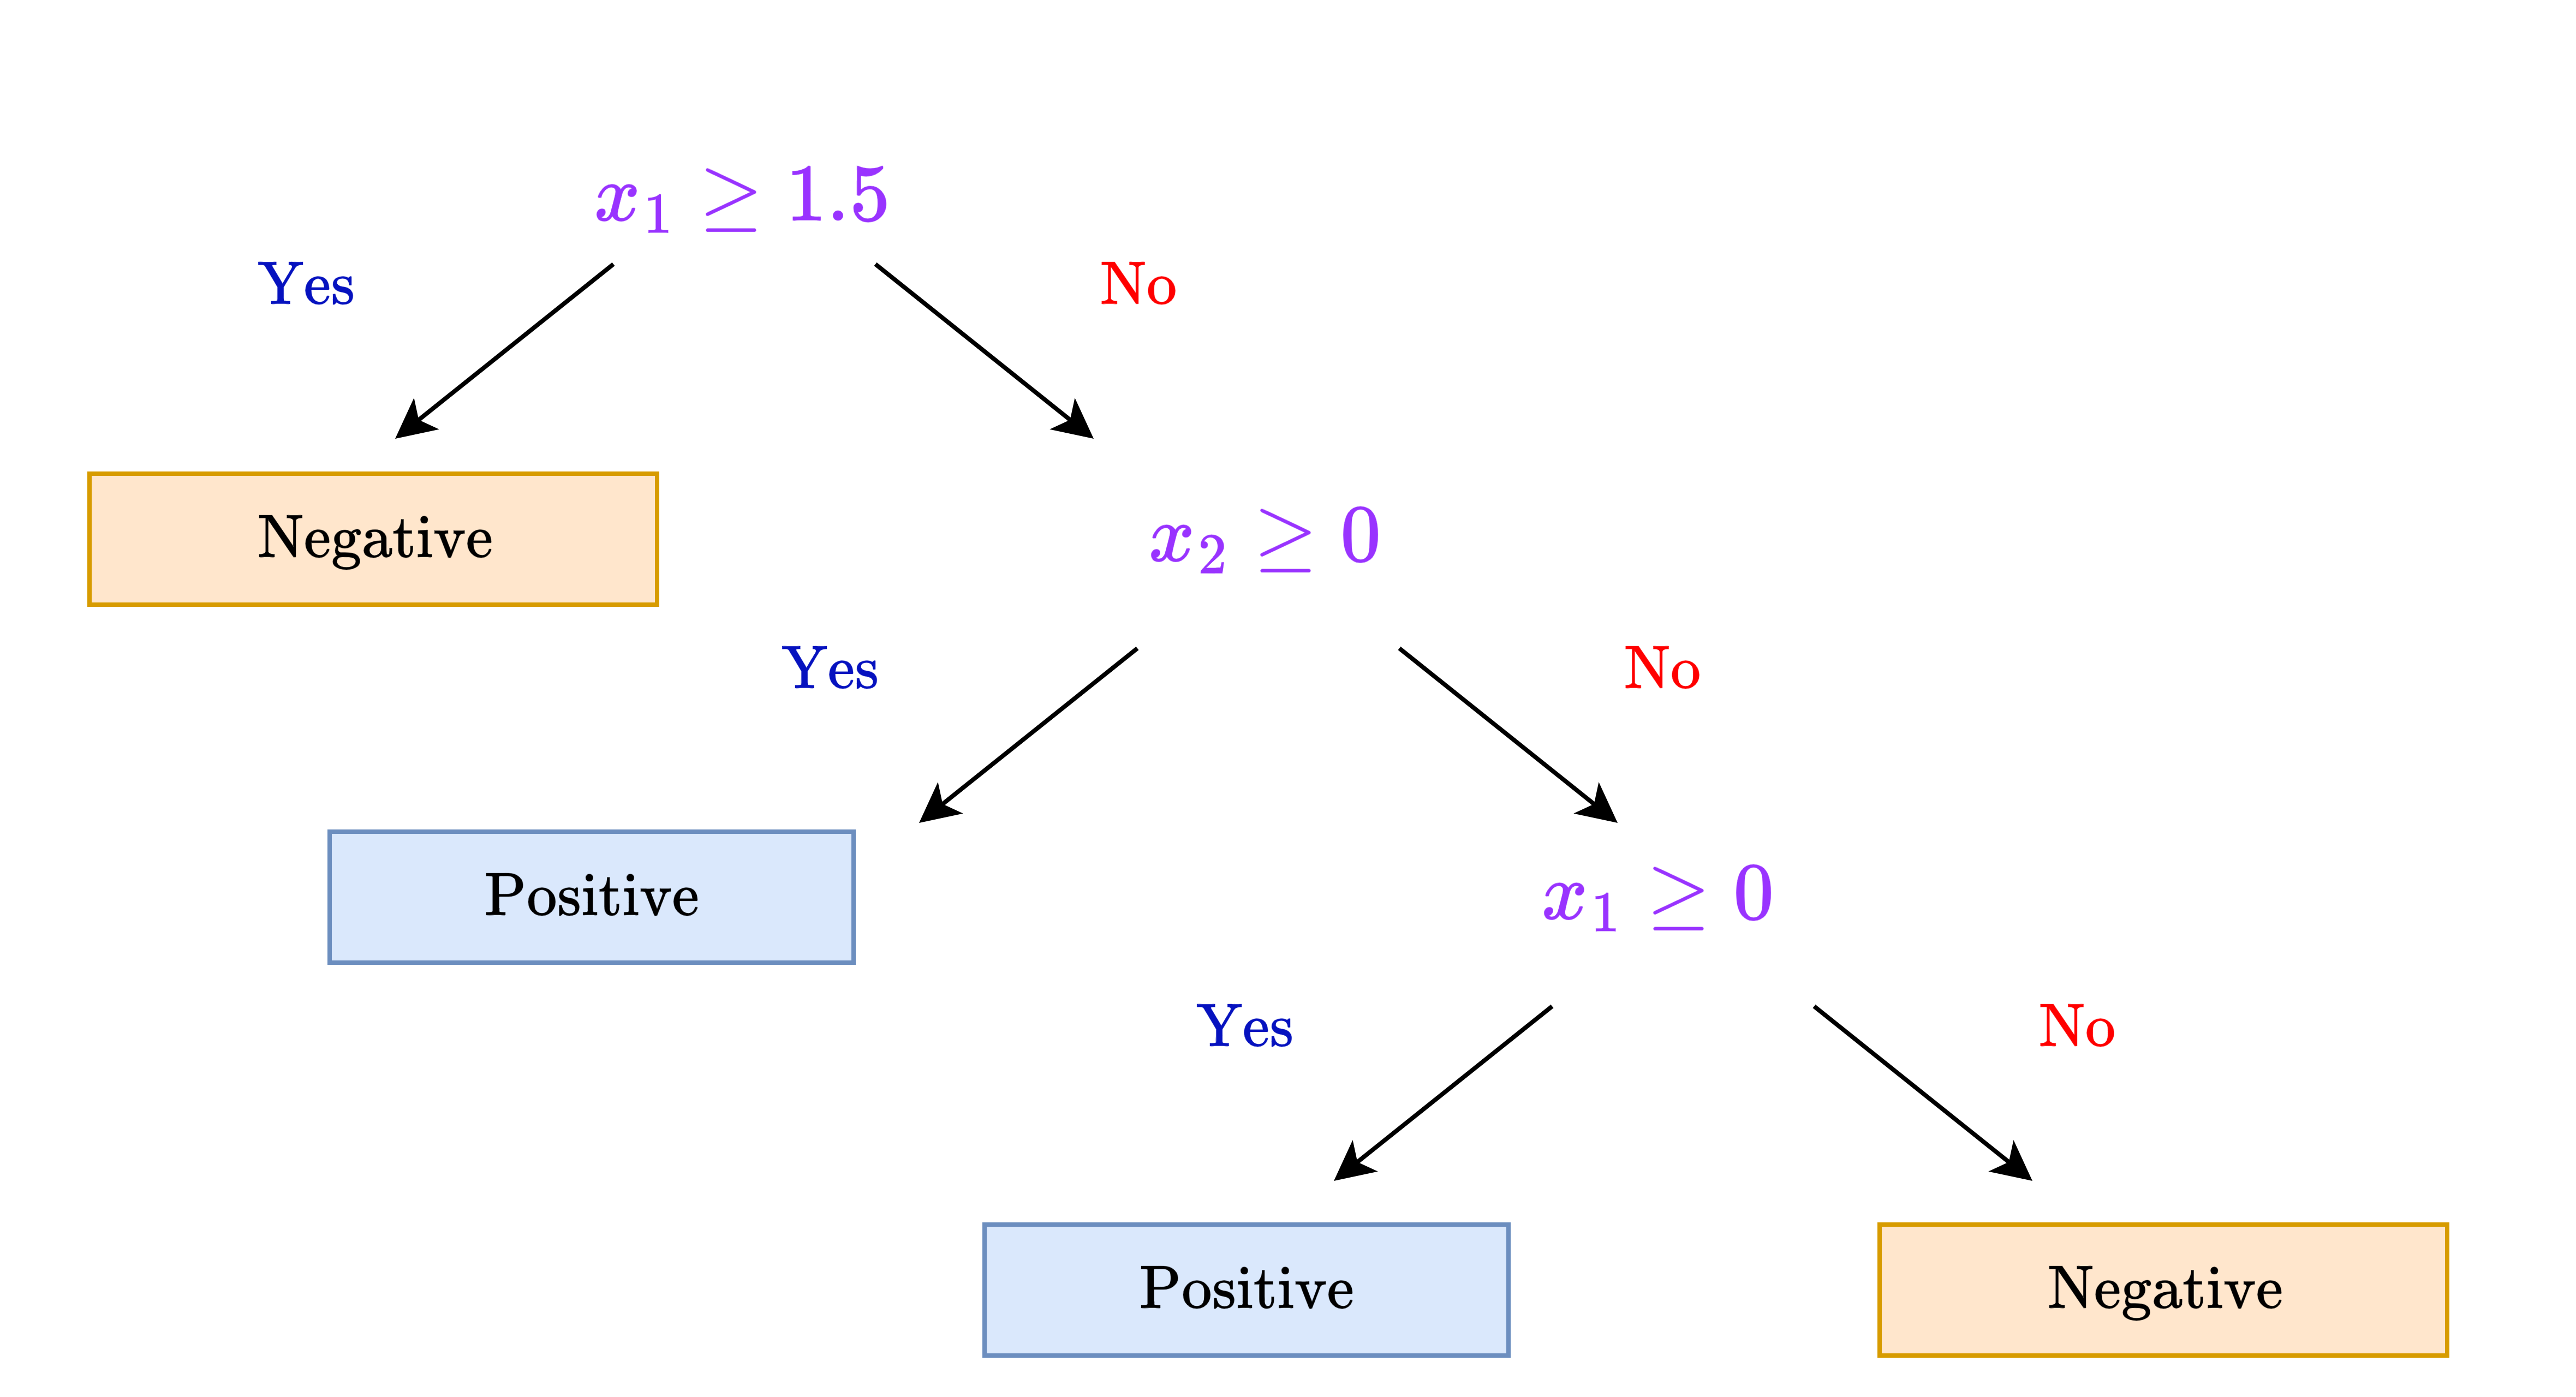
\includegraphics[width=85mm,scale=0.5]{images/nonparametric_images/x1_geq_0_tree.png}
        \end{figure}

        And we're finished! 

        \begin{itemize}
            \item Let's color in our last region.
        \end{itemize}

        \begin{figure}[H]
            \centering
            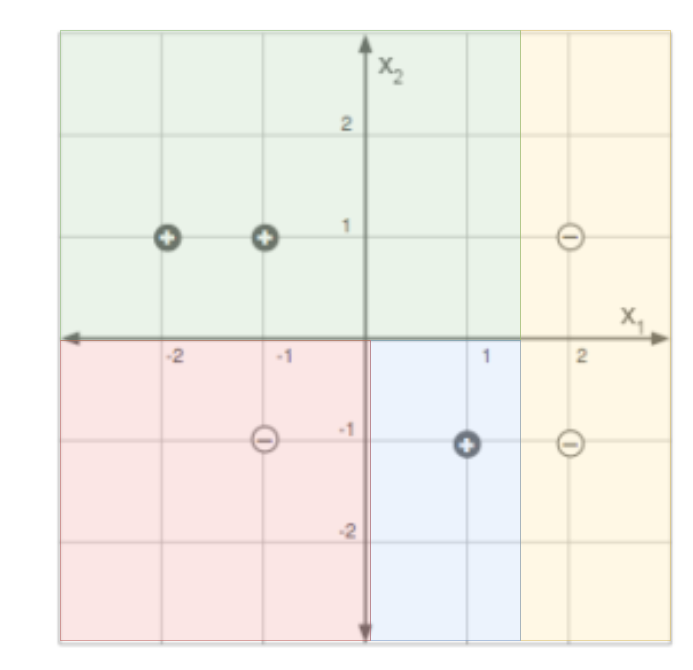
\includegraphics[width=50mm,scale=0.5]{images/nonparametric_images/full_tree.png}
        \end{figure}

        





    \phantom{}

    \subsection{Partitioning: Formalizing our Tree}

        In the above example, we've broken up our input space into chunks, or \vocab{partitions}.\\

        \begin{definition}
            Our tree is used to "\vocab{partition}" our data into multiple different chunks. 

            \begin{itemize}
                \item Thus, we call one of these chunks, a single \purp{partition}. Partitions are the "\gren{leaf nodes}" of our tree.
                \item If we gather all of our partitions together, they should cover the \orgg{whole space}.
            \end{itemize}

            Each of these partitions is assigned a single \gren{constant} $O_m$: every data point in that partition is given this constant as an output.

            \begin{equation*}
                \ex{g}{i} = O_m
            \end{equation*}
        \end{definition}

        \miniex Each of the differently colored regions above is one partition. The red and yellow partitions are assigned "negative", while the green and blue ones are assigned "positive".


        Now that we understand how trees work, we can \purp{formalize} our process, mathematically.

        Our tree does two things:

        \begin{itemize}
            \item Put each data point in \purp{one partition} $R_m$. 
                \note{This is one of our regions, after splitting up the space.}

            \item Give each partition an \gren{output value} $O_m$.
            
            \begin{itemize}
                \item This is the output we'll use for any data point in this partition.
            \end{itemize}
        \end{itemize}

        These two parts make up our \vocab{predictor}.\\

        \begin{definition}
            Suppose our tree creates $M$ distinct partitions. The \vocab{predictor} generated by our \gren{tree} has two main parts:

            \begin{itemize}
                \item A \vocab{partition function} $\pi$: this function assigns each point $x$ in the \gren{input space} to a \purp{partition} $R_m$.

                \item A \vocab{collection of outputs} $O$: the $\nth{m}$ \gren{output}, $O_m$, is assigned to \purp{all points} $x$ in region $R_m$.
            \end{itemize}
        \end{definition}

        Each of our training data is assigned to one partition, by the partition function.

        \begin{equation}
            \grn{\pi} \big(  \; \blu{\ex{x}{i}} \; \big)=\pur{R_m} \qquad \implies \qquad \grn{\ex{x}{i}} \in \pur{R_m}
        \end{equation}

        \begin{figure}[H]
            \centering
            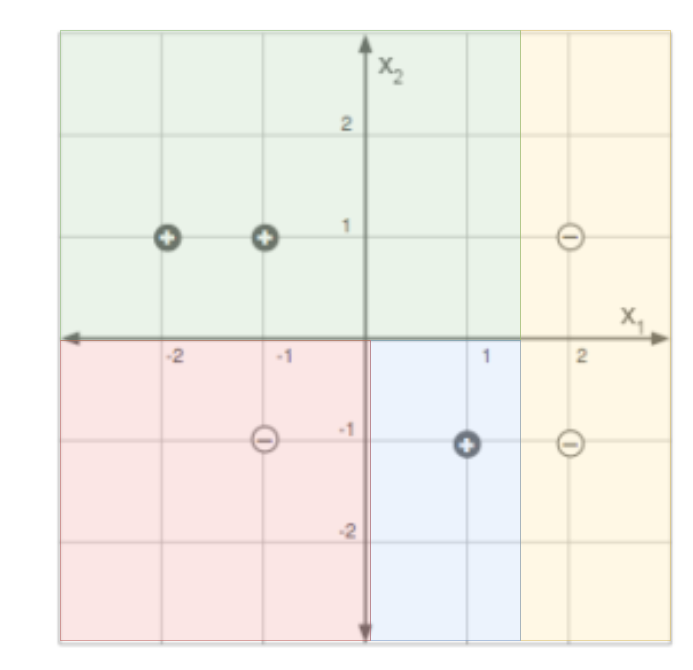
\includegraphics[width=50mm,scale=0.5]{images/nonparametric_images/full_tree.png}
            \caption*{The data point at $(2,1)$ is assigned to the yellow partition. Since we created it first, we could call the yellow partition $R_1$. If we classify either -1 or +1, we should choose $O_1=-1$.}
        \end{figure}


    \pagebreak

    \subsection{Regression}

        Now, we want to show how to measure, and create this tree. We'll start with the problem of \vocab{regression}.

        \begin{figure}[H]
            \centering
            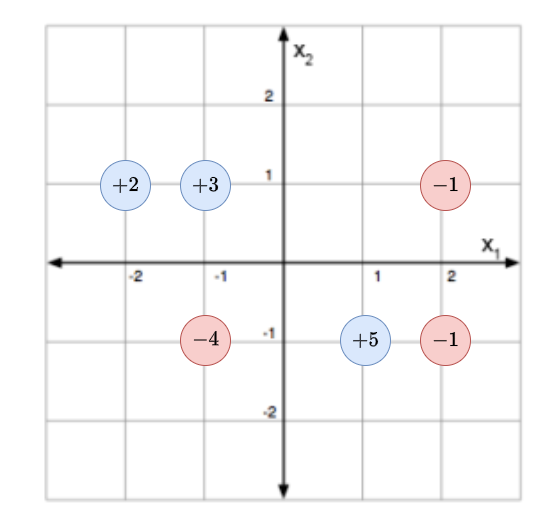
\includegraphics[width=50mm,scale=0.5]{images/nonparametric_images/regression_example.png}
            \caption*{For regression, our values aren't categorical: they're real numbers. We used integers here, but we could've used $2.5$ or $-\sqrt{2}$.}
        \end{figure}


        What output value do we give for $O_m$? Typically, the most accurate option would be the \gren{average} of all outputs $\ex{y}{i}$ for data points in region $R_m$.

        

        \begin{itemize}
            \item But we only want to include the data points $\big( \ex{x}{i}, \ex{y}{i} \big)$ where $\pur{\ex{x}{i} \in R_m}$. 
            \item To simplify things, we'll refer to each data point by its index.\\
        \end{itemize}

        \begin{notation}
            Each training data point is referenced by its \gren{index} $i$. So, rather than \orgg{partitioning} $\ex{x}{i}$, we'll partition indices $i \in I$.

            \begin{itemize}
                \item The training data which are \purp{included} in $R_m$, will have their indices included in $I_m$.
            \end{itemize}

            

            \begin{equation*}
                \ex{x}{\red{i}} \in R_m \qquad \iff \red{\qquad i \in I_m}
            \end{equation*}
        \end{notation}

        We can use this to take our average.\\

        \begin{definition}
            In \vocab{regression}, $O_m$ is the \gren{average} of all outputs $\ex{y}{i}$ for training data in \purp{partition} $R_m$.

            \begin{itemize}
                \item So, we only include the data points $\ex{x}{i}$ relevant to $R_m$.
            \end{itemize}

            \begin{equation*}
                \grn{O_m} = 
                \operatorname{Average}_{\red{i \in I_m}} \Big( \org{\ex{y}{i}} \Big) 
            \end{equation*}

            or,

            \begin{equation*}
                \grn{O_m} = 
                \operatorname{Average} \Big( \quad \Big\{ 
                    \org{\ex{y}{i}} \quad \text{ if } \quad \pur{\ex{x}{i} \in R_m} 
                \Big\} \quad  \Big)
            \end{equation*}

        \end{definition}

        \miniex Consider the following split.

        \begin{figure}[H]
            \centering
            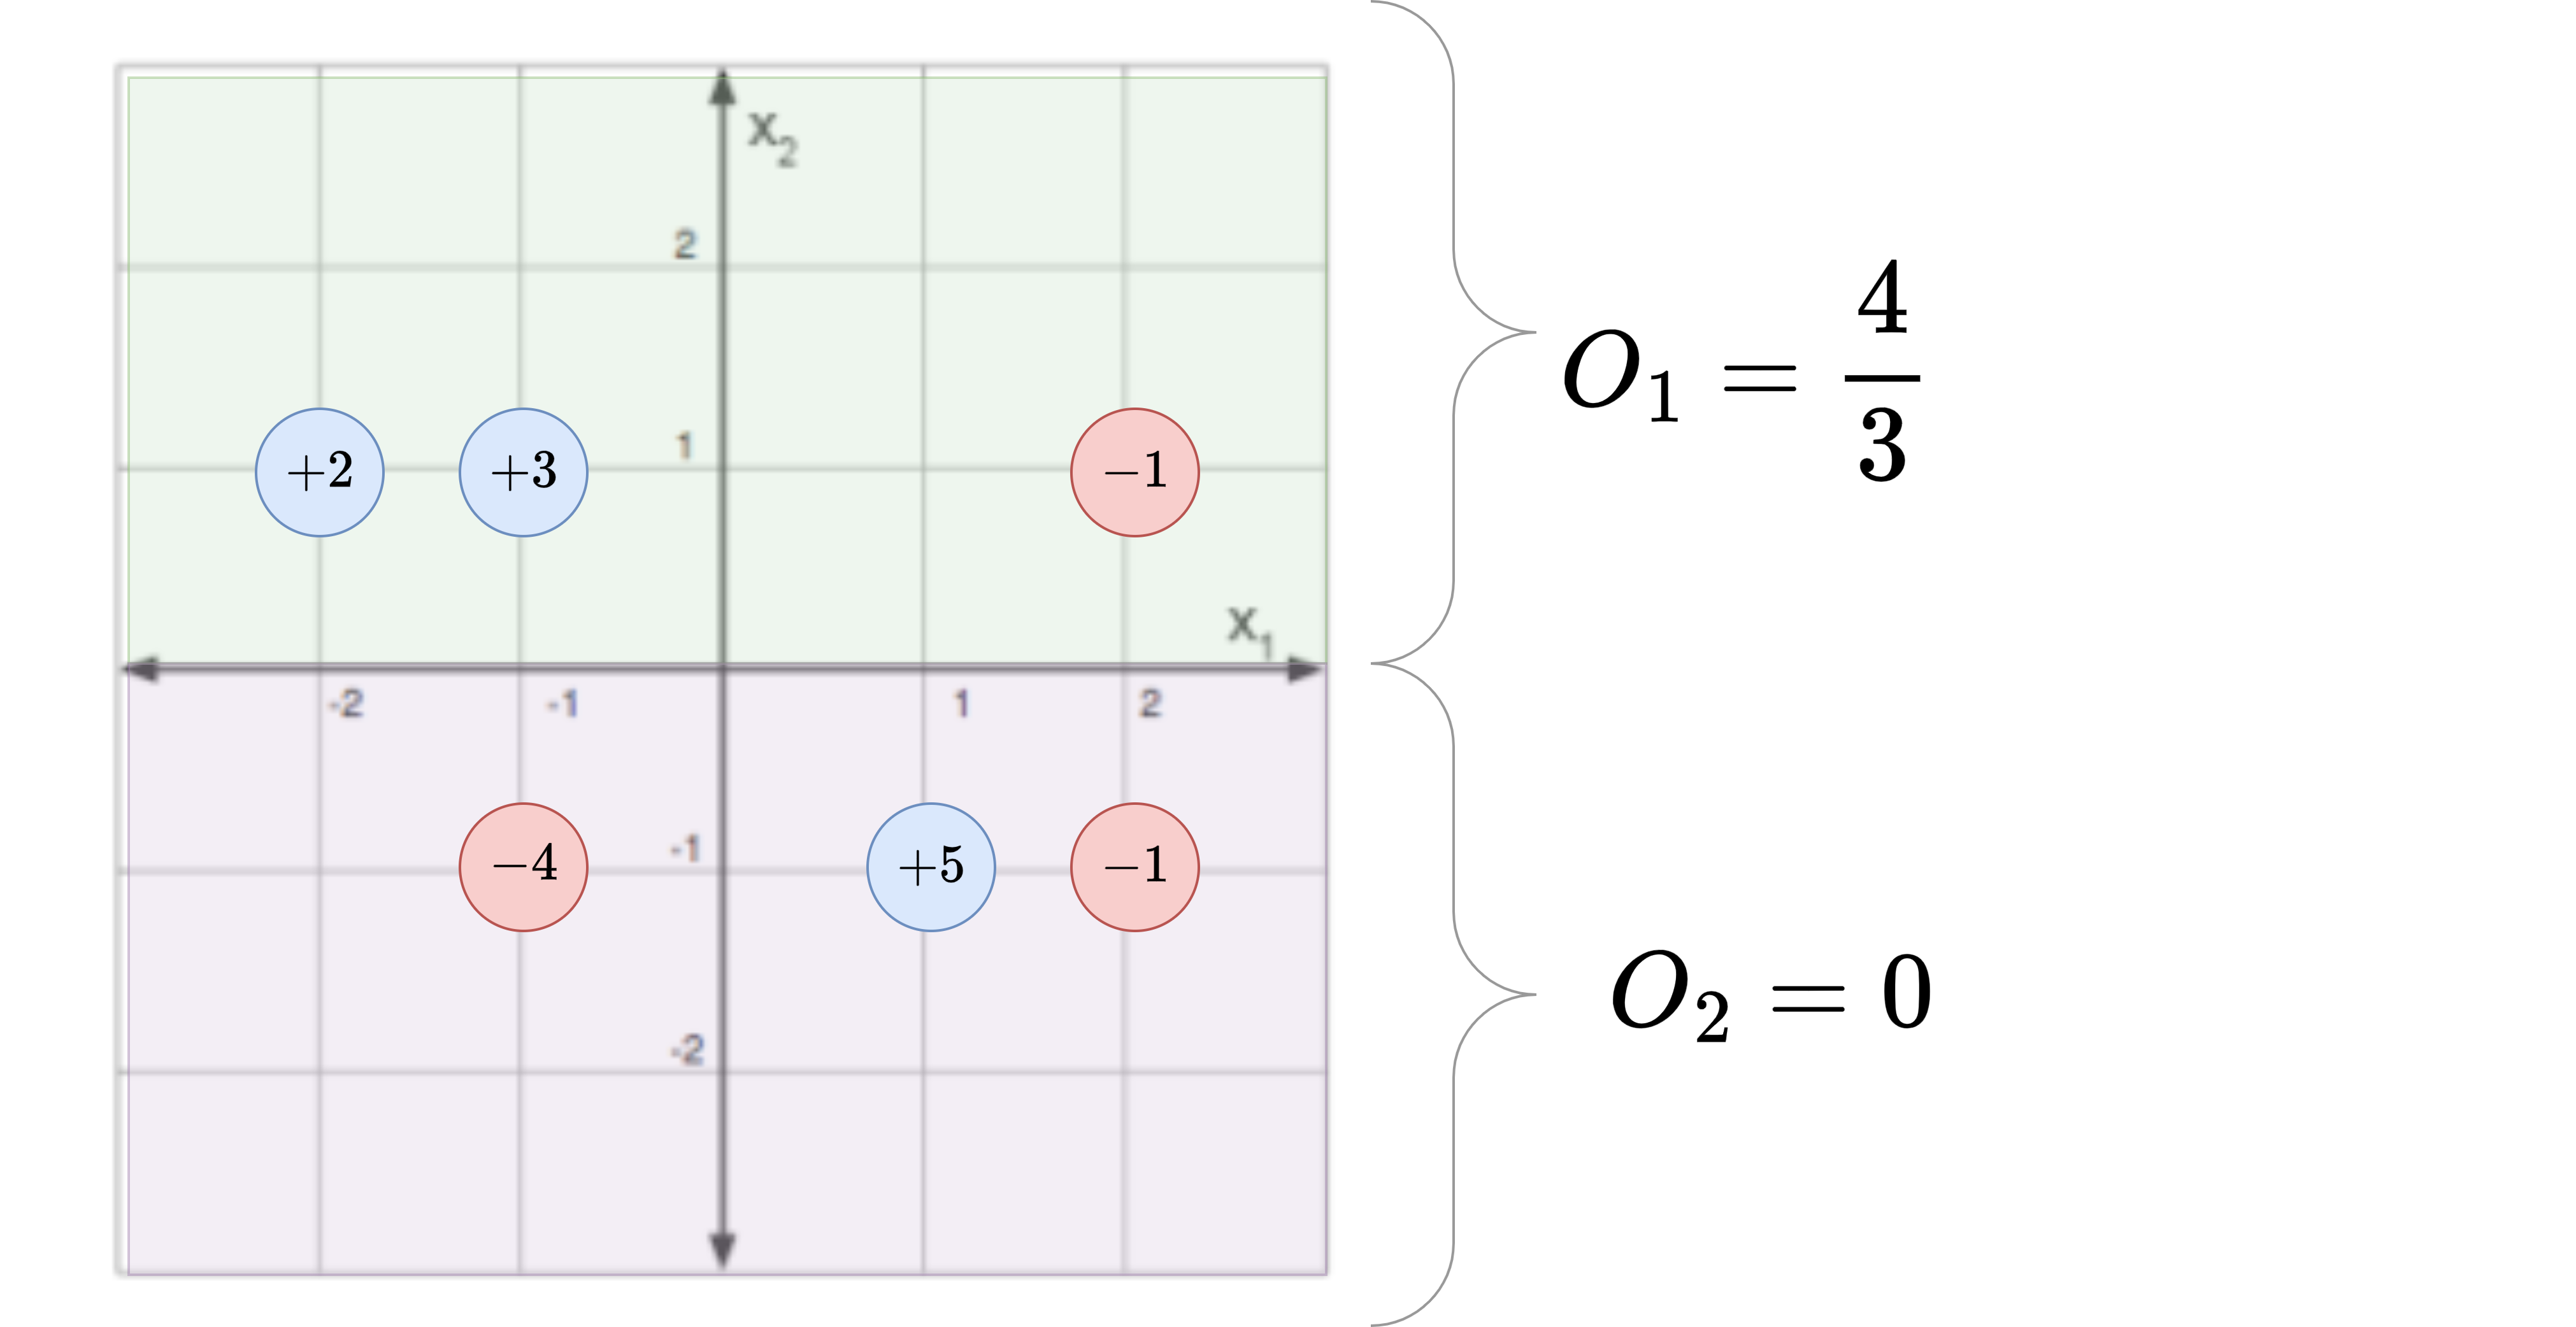
\includegraphics[width=90mm,scale=0.5]{images/nonparametric_images/x2_split_averaged.png}
            \caption*{We create a split at $x_2=0$. For each region, we average the value of all elements.}
        \end{figure}




    \phantom{}

    \subsection{Regression Loss}

        How do we measure our loss? Same as usual for regression: we use \purp{squared error}.\\

        \begin{definition}
            The \vocab{regression loss} for our region $R_m$ is given by the \gren{squared error} between our guess and the answer.
            
            \begin{itemize}
                \item We guess $\grn{O_m}$ for every data point in region $R_m$.
            \end{itemize}

            \begin{equation*}
                E_m = \sum_{\red{i \in I_m}} \big( \grn{O_m} - \org{\ex{y}{i}} \big)^2
            \end{equation*}
        \end{definition}

        To get our loss, we could add up this loss over all of our regions.
            \note{If you want to practice with the above example, the error is $152/3$.}

        \begin{equation}
            \loss_{err} = \sum_{m=1}^M E_m
        \end{equation}

        But we have a concern: \purp{overfitting}. What if we create too many regions? That wouldn't be very helpful.

        \begin{figure}[H]
            \centering
            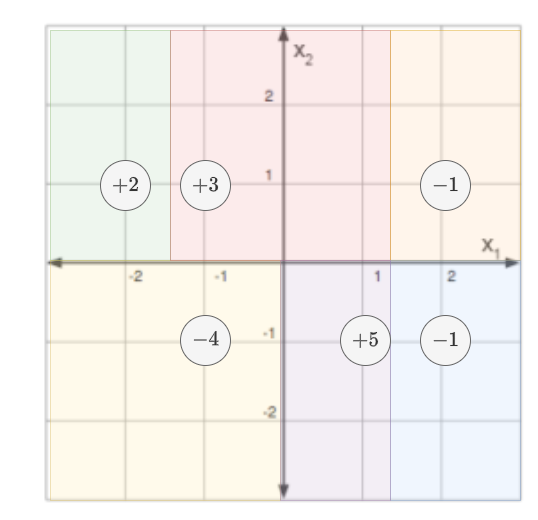
\includegraphics[width=50mm,scale=0.5]{images/nonparametric_images/overfit_example.png}
            \caption*{If we wanted to, we could create a partition for every \textbf{single data point}. 100\% accuracy.}
        \end{figure}

        This especially becomes a problem as we get a \purp{larger dataset}: having a partition for every piece of training data will make you incredibly \gren{sensitive to noise}.

        So, we want to \textit{discourage} this kind of behavior.\\

        \begin{concept}
            To reduce \purp{overfitting}, we'll include a \vocab{regularization term} that discourages having too many regions.

            \begin{itemize}
                \item Our number of regions is $M$, so we want to \orgg{penalize} this: we'll add it to our loss function.
            \end{itemize}

            \begin{equation*}
                \loss_{reg} = \lambda M
            \end{equation*}

            \subsecdiv

            $\lambda$, similar to ridge regression, is used to indicate how strongly we want to \gren{regularize}:

            \begin{itemize}
                \item Too high $\lambda$ can result in \purp{underfitting}: we get structural error, not splitting enough to accurately represent our data.
                \item Too low $\lambda$ can result in \orgg{overfitting}: we split more than we need, focusing on noise in the data.
            \end{itemize}
        \end{concept}

        Combining these, we find our loss function for tree-based regression.\\

        \begin{kequation}
            The \vocab{objective function} for \gren{tree}-based regression has two parts:

            \begin{itemize}
                \item Loss $\loss_{err}$, telling us how \purp{inaccurate} our predictions are.
                \item Regularization $\loss_{reg}$, penalizing us for having \gren{too many splits}, and overfitting.
            \end{itemize}

            \begin{equation*}
                J = \org{\loss_{err}}+\blu{\loss_{reg}} \quad = \quad \org{\sum_{m=1}^M E_m} + \blu{\lambda M}
            \end{equation*}

            Where

            \begin{equation*}
                E_m = \sum_{\red{i \in I_m}} \big( \grn{O_m} - \org{\ex{y}{i}} \big)^2
                \qquad \qquad \qquad
                \grn{O_m} = 
                \operatorname{Average}_{\red{i \in I_m}} \Big( \org{\ex{y}{i}} \Big) 
            \end{equation*}
            
        \end{kequation}

        It's possible to search all partitions of our training data, and find the best one directly.

        \begin{itemize}
            \item But this is NP-hard. All you need to know is that it's incredibly time-consuming.\\
        \end{itemize}

        \begin{concept}
            For large training sets, it's often \gren{too expensive} to try all possible partitions of our training data.

            Since partitions also aren't \purp{smooth}, it'll be difficult to find the \orgg{optimal} solution via gradient descent.
        \end{concept}

        So, instead, we'll come up with a (greedy) algorithm to find a pretty good solution.





    \pagebreak
        

    \subsection{Greedy algorithms}

        We need to design a tree-building algorithm. Our easiest bet is to be \gren{greedy}:\\

        \begin{definition}
            A \vocab{greedy algorithm} is one that takes the choice that looks best, \gren{immediately}.

            \begin{itemize}
                \item It doesn't factor in the \purp{future} effects of our decision.
            \end{itemize}
        \end{definition}

        \miniex In an MDP problem, this would be like looking for the best immediate reward $R(s,a)$, without at all consider what our future rewards look like.

        This is a very rough approach, but it's much faster than trying every possibility.




    \phantom{}

    \subsection{How to be greedy}

        So, we does our "greedy" choice look like? 

        \begin{itemize}
            \item Our first thought might to be to try every possible split. But our input space is made up of \gren{real numbers}: there are an infinite number of possible splits?
        \end{itemize}

        But are there an infinite number of splits that \textit{matter}?

        \begin{figure}[H]
            \centering
            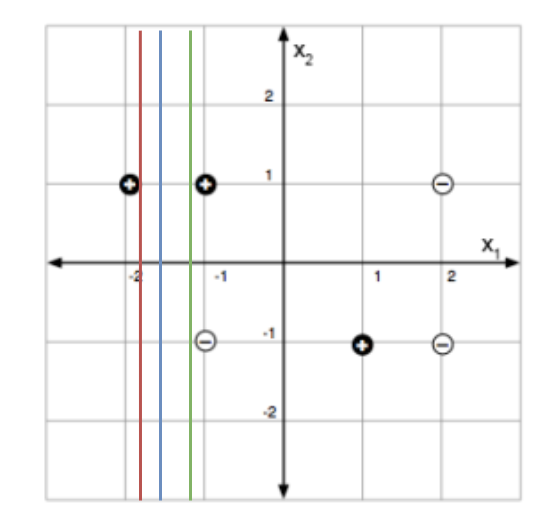
\includegraphics[width=50mm,scale=0.5]{images/nonparametric_images/equivalent_splits.png}
            \caption*{ (Using classification ex., for visual clarity) All three of these splits are the same, as far as our training data is concerned.}
        \end{figure}

        This is useful: we don't have to try every possible split, because some splits are equivalent.

        \begin{itemize}
            \item We only create new splits each time we \purp{move past} a new data point.
            \item So, we can iterate through our splits by going \orgg{one data point} at a time.
        \end{itemize}

        \begin{figure}[H]
            \centering
            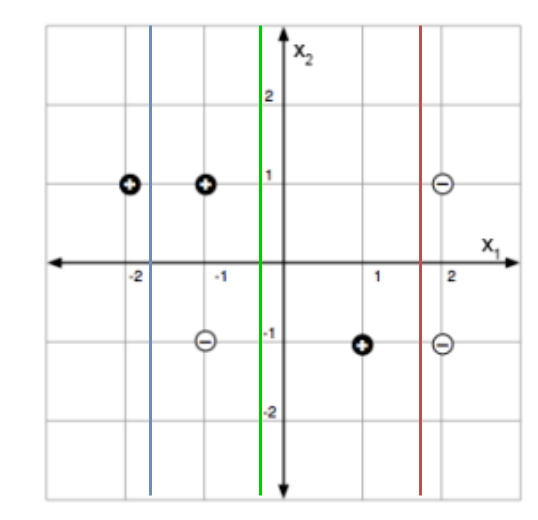
\includegraphics[width=50mm,scale=0.5]{images/nonparametric_images/unique_splits_x1.png}
            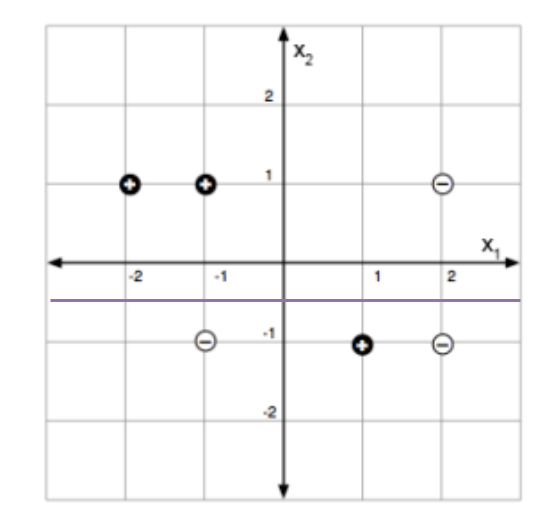
\includegraphics[width=50mm,scale=0.5]{images/nonparametric_images/unique_splits_x2.png}
            \caption*{Here are all of the distinct splits between data points, on our two axes. We only create one split each time we cross data points on an axis.}
        \end{figure}

        This is the complete set of all possible "first splits".
            \note{Notice that we don't need to include splits that have no data on one side of our dataset: these splits do nothing.}

        \begin{itemize}
            \item In order to be greedy, we just try all of these splits, and see which one works best.
                \note{If many splits are equivalent to the ones shown above, how do we know which ones to use?
                
                \phantom{}
                
                Our answer: for this class, we don't really care. If you need a mental image, you can place each split halfway between the closest data points on either side.}\\
        \end{itemize}

        \begin{definition}
            In our \vocab{greedy algorithm} for tree generation, we:

            \begin{itemize}
                \item List every \purp{distinct} split on each axis.

                \item Try every one of these splits, and measure their \orgg{error}.

                \item Choose the split with the \gren{lowest error}.
            \end{itemize}

            After splitting once, we repeat this algorithm in \purp{both halves} of the tree.


            \begin{itemize}
                \item And, once we've split a second time, we split all quarters.

                \item We repeat this process \vocab{recursively}.
            \end{itemize}

        \end{definition}

        One thing left: \purp{termination}.

        \begin{itemize}
            \item We need a stopping point: if we don't terminate, then we'll continue until \gren{every data point} has its own region.\\
        \end{itemize}
        

        \begin{definition}
            We \vocab{terminate} one region of our tree-building algorithm if that region has \purp{fewer than} $k$ data points in it.

            \begin{itemize}
                \item Suppose that $I_m$ gives us all of the \redd{indices} in a particular region. We terminate when:  
            \end{itemize}

            \begin{equation*}
                \big| I_m \big| \leq k
            \end{equation*}

            $k$ is a \orgg{hyperparameter}.
        \end{definition}

        Now, our algorithm is complete. 

        


    \pagebreak

    \subsection{Tree regression pseudocode}

        We can also write this as pseudocode. But, let's establish some notation:\\

        \begin{notation}
            For this section, each split occurs on \purp{dimension $j \in J$}, at \gren{position $s \in S_j$}.

            \begin{equation*}
                x_j \geq s
            \end{equation*}
        \end{notation}

        We're ready to go.
            \note{Below, we use $\pur{i \in I^+[j,s]}$ to filter for the data points \purp{above} the split, and $\grn{i \in I^-[j,s]}$ to filter for the data points \grn{below} the split.}

        \begin{codebox}
            \Procname{$\proc{BuildTree}( I, k)$}
            \li  \If $\big| I \big| \leq k$ 
                 \qquad \qquad \lblu{ \# If fewer than $k$ data points: no splitting}
                 \Then
            \li
            
            \li    $\org{ \hat{y} } = {\rm Average}_{\pur{i \in I}} \big( \ex{g}{i} \big)$ 
                \qquad \qquad \lblu{ \# Final output }
            \li    \Return $\proc{Leaf} \big( \org{ \text{output} =  \hat{y} } \big)$
                \qquad \qquad \lblu{ \# Leaf node: no more splits }
            \li
            
            \li  \Else
                \qquad \qquad \qquad \qquad \lblu{ \# Try every possible split }
            \li   \For dim \blu{$j$} in \blu{$J$} 
                \qquad \qquad \qquad \qquad \lblu{ \# Check each dimension }\Do
                \li    \For value \red{$s$} in \red{$S_j$} 
                    \qquad \qquad \qquad \qquad \lblu{ \# Check each split on dim $j$ }\Do
                    \li     
                    \li $I^+\big[j,s\big] = \setty{ \pur{i \in I}  \;\; \Big| \;\; \red{x_j^{(i)} \geq s} }$ 
                        \qquad \qquad \lblu{ \# Data points "above" the split (j,s)}
                    \li
                    \li $I^-\big[j,s\big] = \setty{  \grn{i \in I}  \;\; \Big| \;\; \red{x_j^{(i)} < s} }$ 
                        \qquad \qquad \lblu{ \# Data points "below" the split (j,s)}

                    \li
                    \li $\org{ \hat{y}^+ } = {\rm Average}_{\pur{i \in I^+[j,s]}} \quad 
                    \big( \ex{g}{i} \big)$ 
                        \qquad \qquad \lblu{ \# Output "above" the split }
                    \li $\org{ \hat{y}^- } = {\rm Average}_{\grn{i \in I^-[j,s]}} \quad 
                    \big( \ex{g}{i} \big)$ 
                        \qquad \qquad \lblu{ \# Output "below" the split }

                    \li 

                    \li $\bro{E^+} = \sum_{\pur{i \in I^+[j,s]}} \quad
                    \big( \; \org{\hat{y}^+} - \ex{y}{i} \;\big)^2$
                    \li $\bro{E^-} = \sum_{\grn{i \in I^-[j,s]}} \quad
                    \big( \; \org{\hat{y}^-} - \ex{y}{i} \; \big)^2$
                    \li $\bro{E\big[j,s\big]} = E^+ + E^-$
                        \qquad \qquad \qquad \qquad \lblu{ \# Error for this split }
                    \li
                \End
                \End
        \li   $(\red{j^*}, \grn{s^*}) = 
               {\rm arg~min}_{\blu{j},\red{s}}   \big( \; \bro{E} \big[j,s \big] \; \big)$
            \qquad \qquad \lblu{ \# Pick split (j,s) with lowest error }
            
            \End
        \li
        \li\lblu{ \# Recursion step}
        \li left\_branch $\;\;\,=  \proc{BuildTree}\big( \;\; I^-\big[\blu{j^*},\red{s^*}\big], \; k \;\;\big) $
            \qquad \qquad \lblu{ \# Split the left/lower half of data }
        \li right\_branch $= \proc{BuildTree}\big( \;\; I^+\big[\blu{j^*},\red{s^*}\big], \; k \;\;\big) $
            \qquad \qquad \lblu{ \# Split the right/upper half of data }
        \li
        \li    \Return $\proc{Node}(\blu{j^*},\red{s^*}, \;\operatorname{left\_branch}, \;\operatorname{right\_branch})$
            \qquad \qquad \lblu{ \# Our node contains the split, and the two halves after the split}
        \end{codebox}



    \subsection{Pruning}

        It's possible that our tree has more branches than it needs. There are a couple ways we might try to avoid this:
        
        \begin{itemize}
            \item Set $k$ relatively \gren{high}, 
            \item Stopping when splitting doesn't improve the \purp{error} very much.
        \end{itemize}

        But stopping too early can be a problem:\\

        \begin{concept}
            One problem with \vocab{early stopping} in tree-building, is that some splits aren't obviously, immediately beneficial.

            \begin{itemize}
                \item But with one or two more splits after, they become very useful.
            \end{itemize}
        \end{concept}

        Consider the XOR problem.

        \begin{figure}[H]
            \centering
            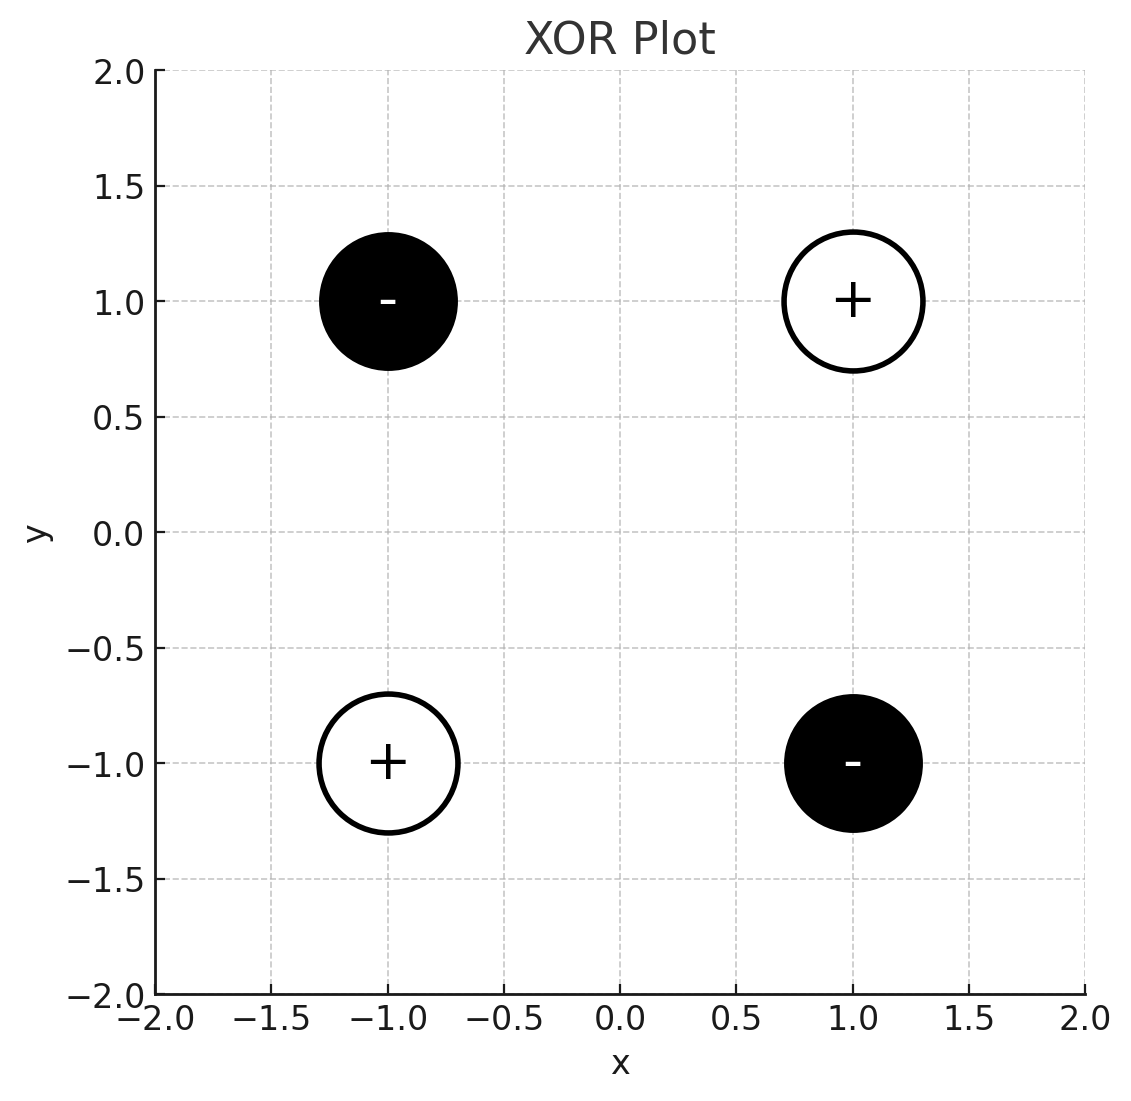
\includegraphics[width=40mm,scale=0.5]{images/nonparametric_images/xor_plot.png}
            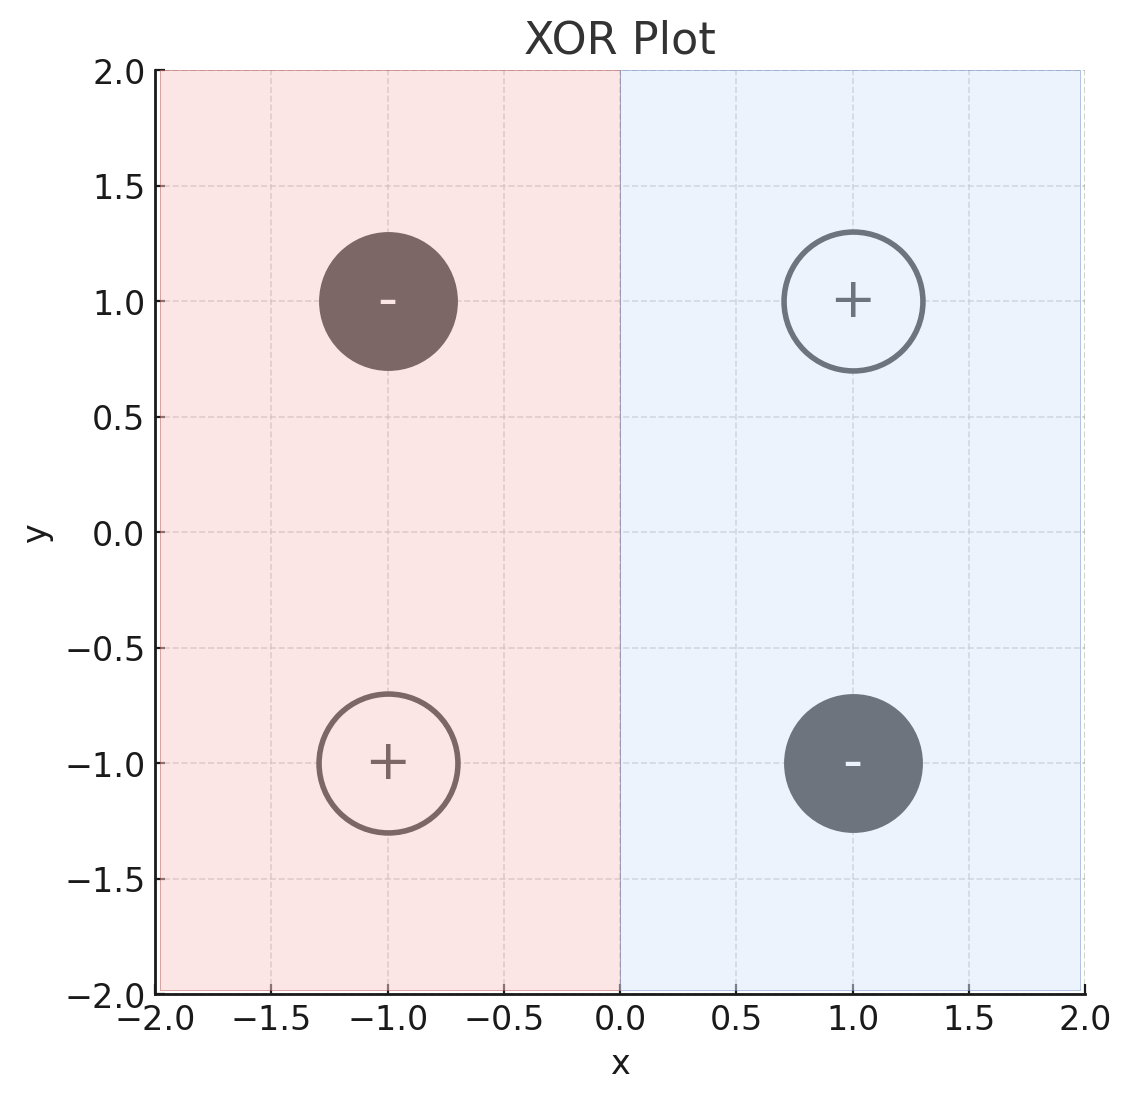
\includegraphics[width=40mm,scale=0.5]{images/nonparametric_images/xor_1split.png}
            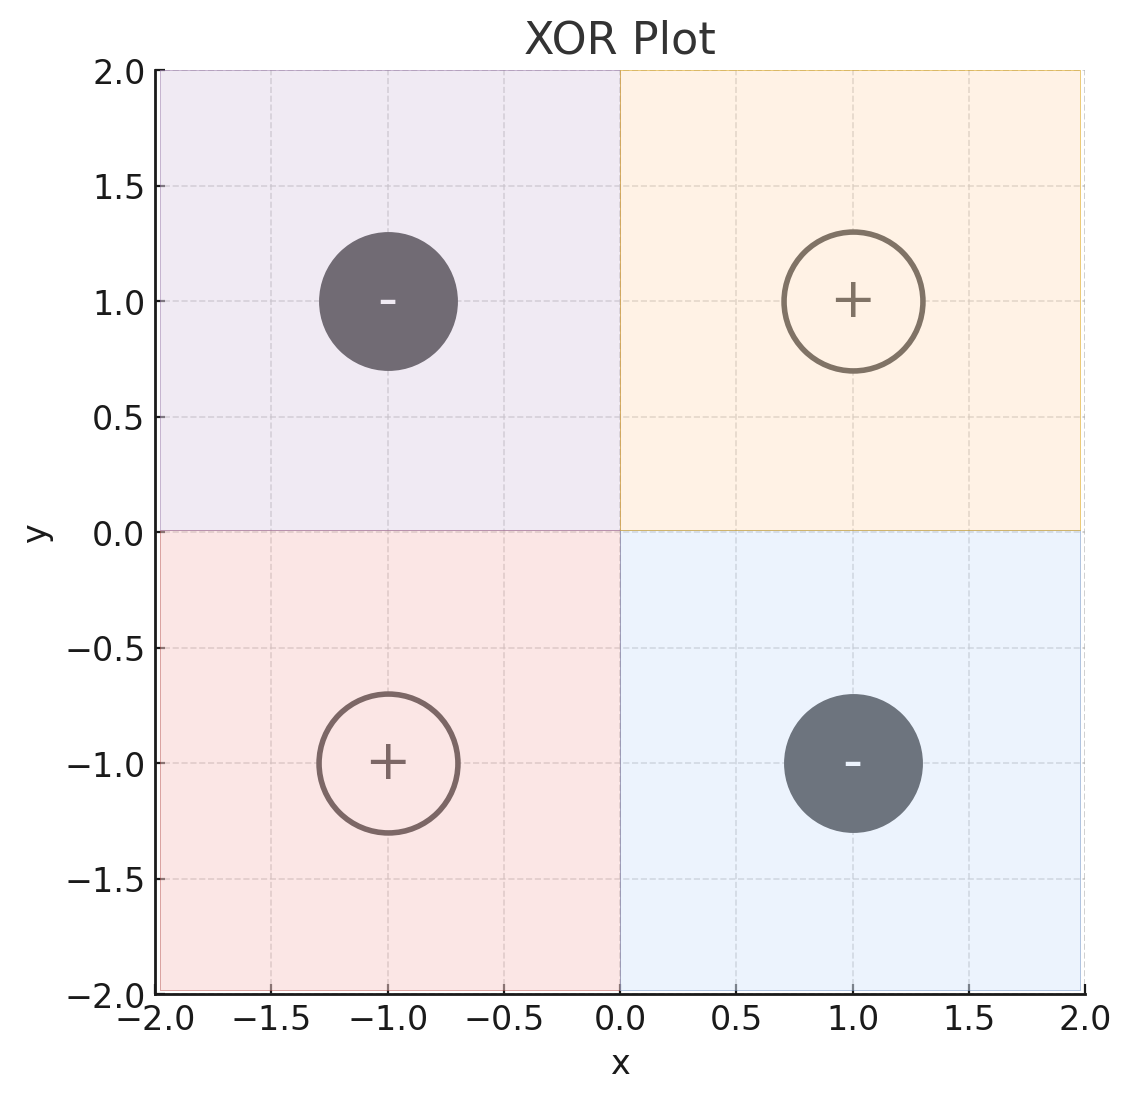
\includegraphics[width=40mm,scale=0.5]{images/nonparametric_images/xor_2split.png}
            \caption*{With only one split, the accuracy isn't any better. But with two splits, we've fixed our problem!}
        \end{figure}

        So, rather than stopping early, it's better to make too many splits, and then \vocab{prune}.\\

        \begin{definition}
            \vocab{Pruning} is to remove \purp{branches} from your \gren{tree}.

            \begin{itemize}
                \item We remove the "\orgg{lowest level}" branches first: splits that create two leaves.
            \end{itemize}
        \end{definition}

        \miniex Consider our examples from earlier in the chapter.

        \begin{figure}[H]
            \centering
            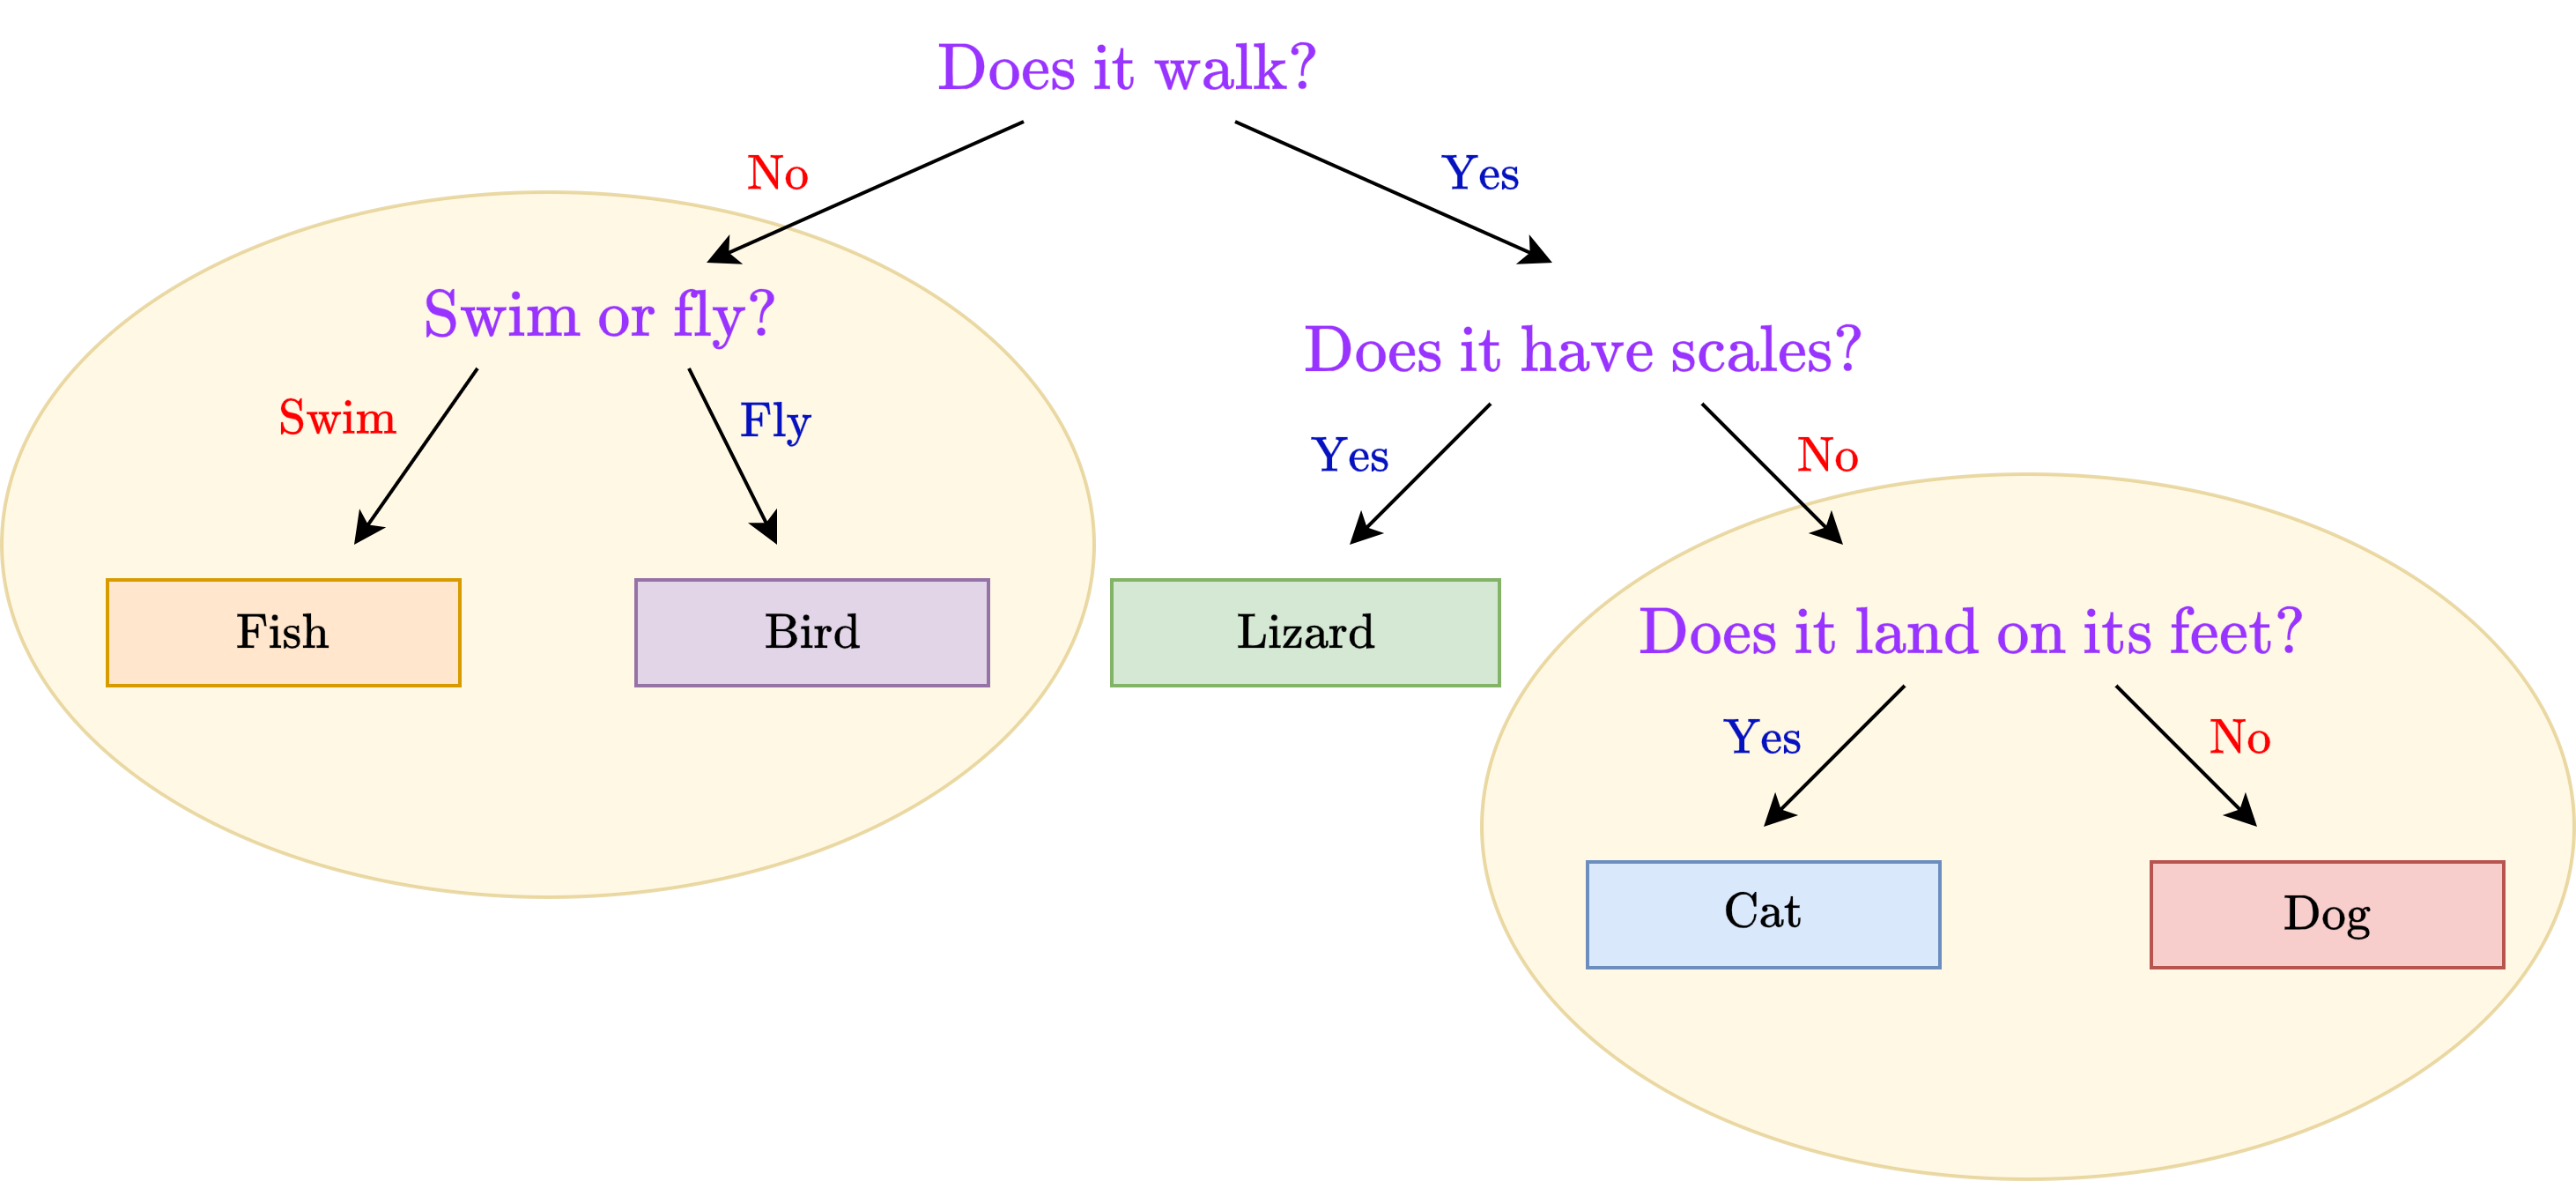
\includegraphics[width=70mm,scale=0.5]{images/nonparametric_images/tree_complex_prune.png}
            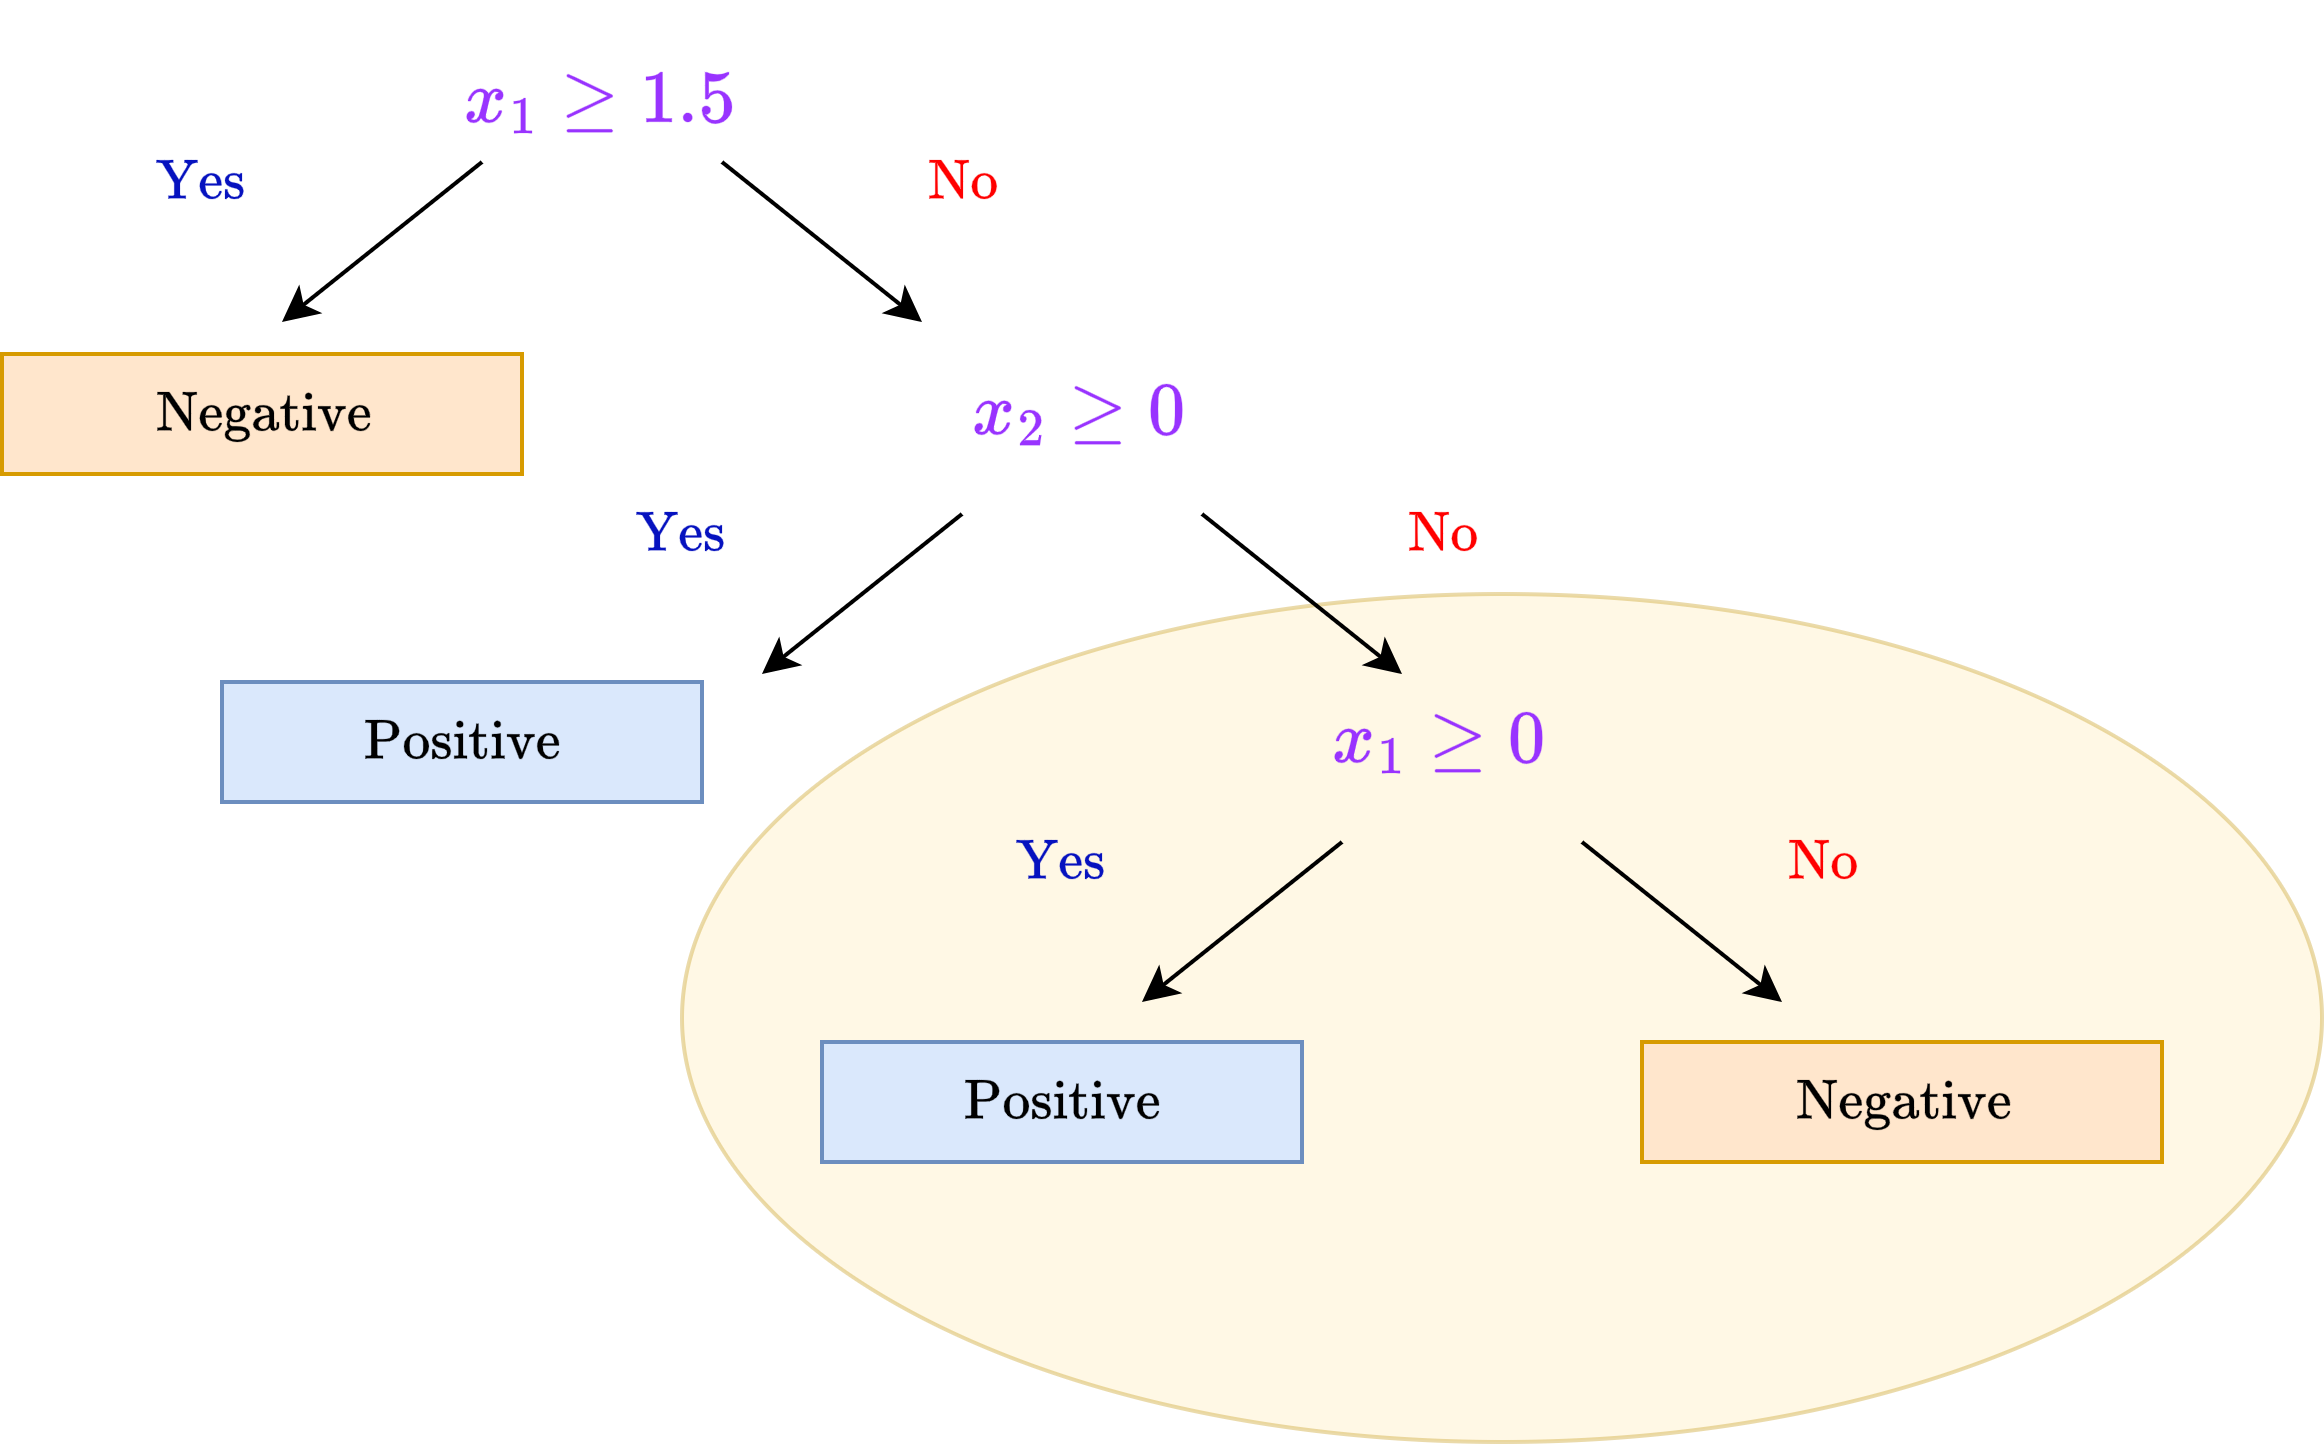
\includegraphics[width=60mm,scale=0.5]{images/nonparametric_images/x1_geq_0_tree_prune.png}
            \caption*{The circled branches on each tree are the only ones we can prune.}
        \end{figure}

        Let's prune one from the pet tree:

        \begin{figure}[H]
            \centering
            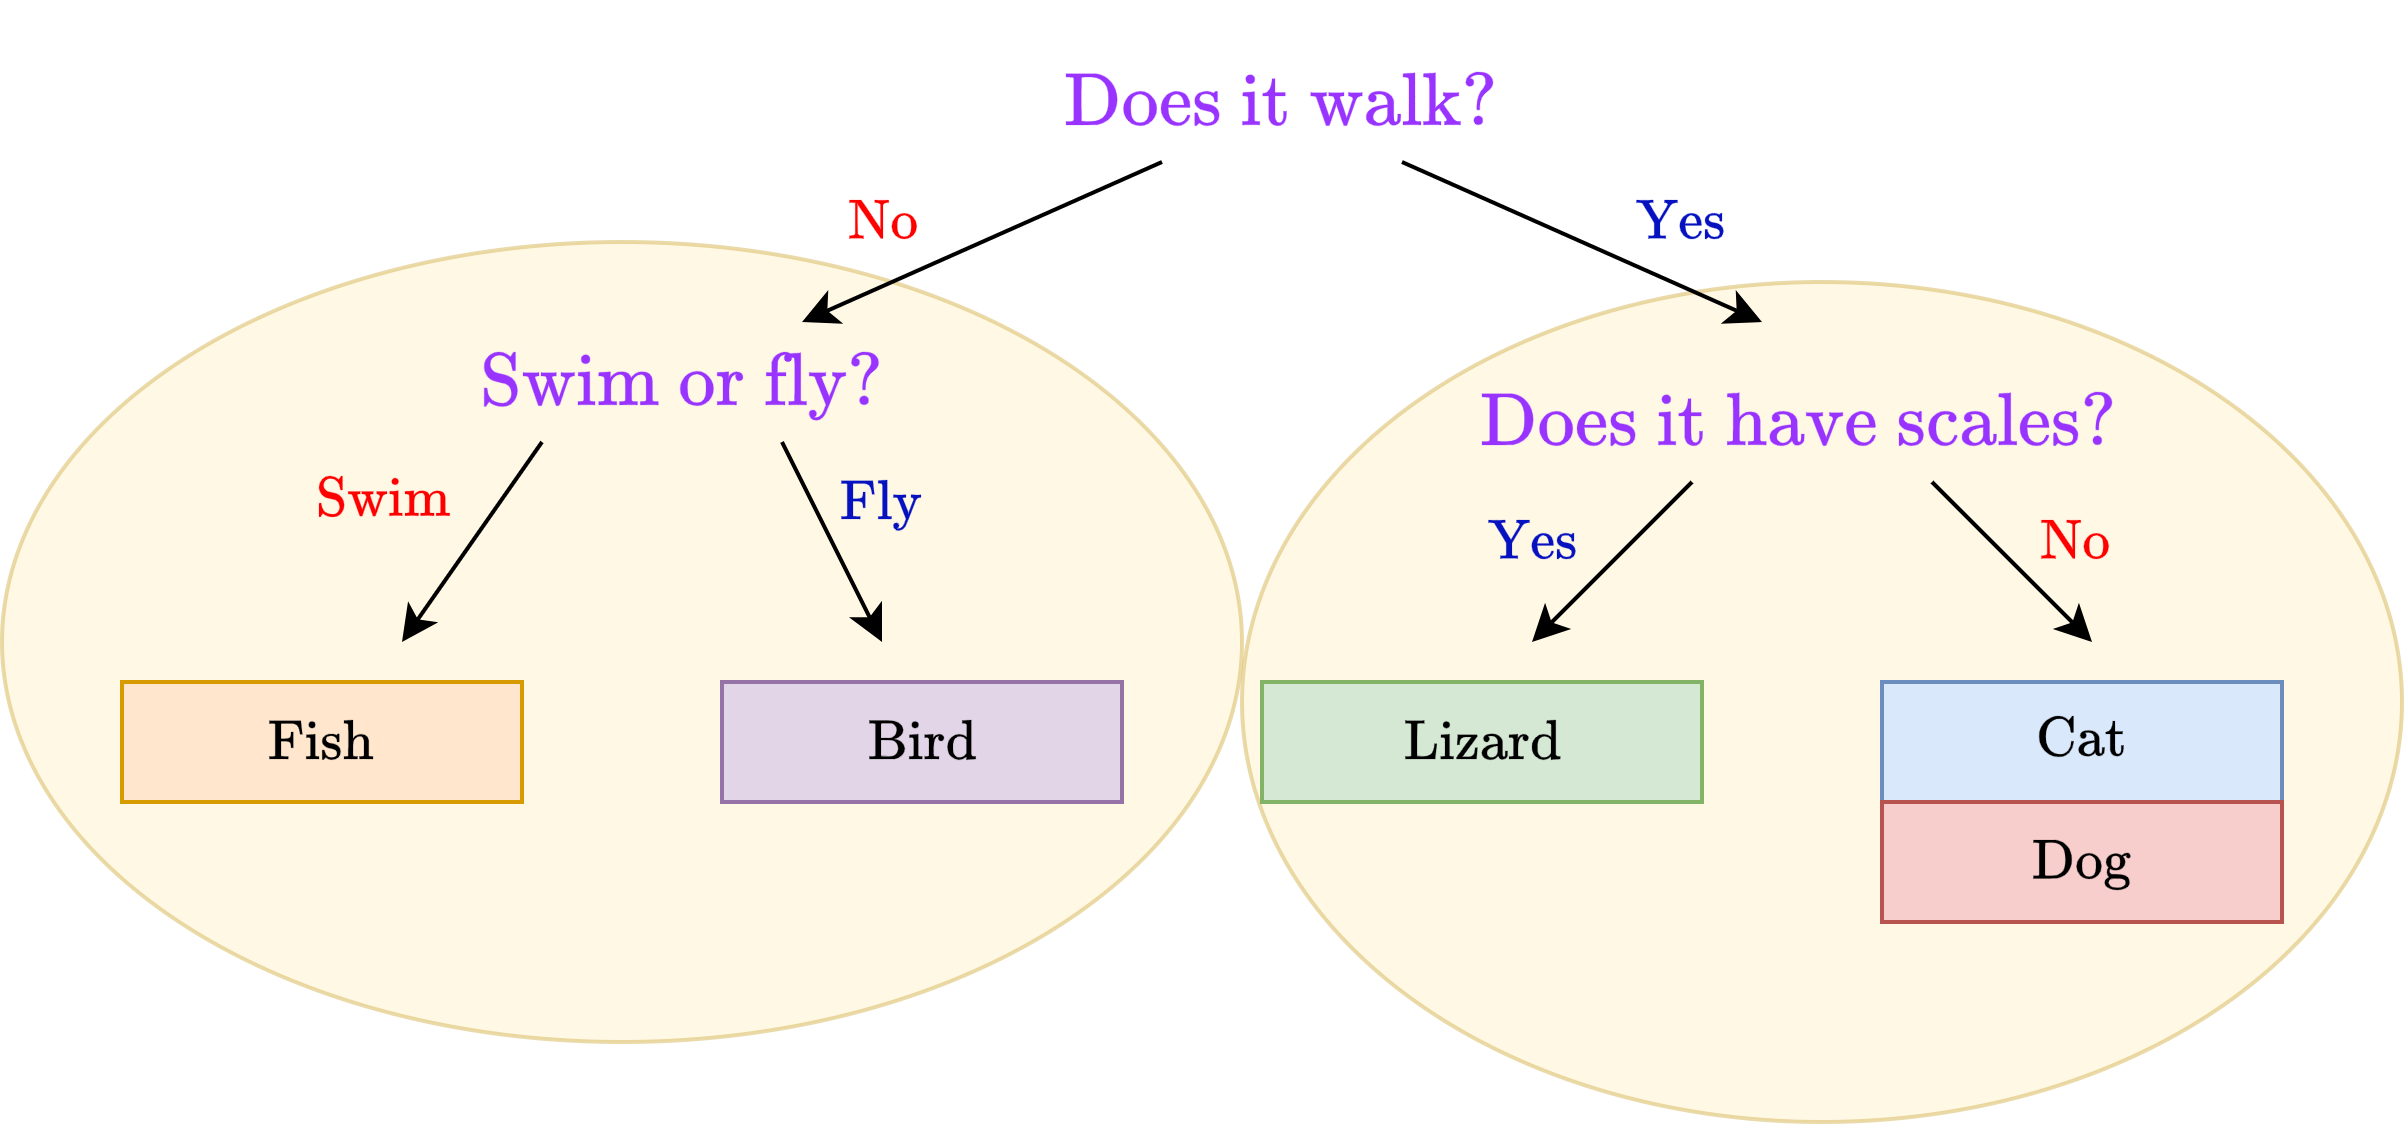
\includegraphics[width=90mm,scale=0.5]{images/nonparametric_images/tree_complex_pruned.png}
            \caption*{Now that we've pruned the lowest branch, we can prune a new, higher branch.}
        \end{figure}

        How do we decide which branches to prune? With our \purp{objective}:

        \begin{equation}
            J = \quad \org{\sum_{m=1}^M E_m} + \blu{\lambda M}
        \end{equation}

        Here, we use a slightly different notation, so that we can express this as a \gren{function}:
            \note{ML notation is a fickle thing.}\\

        \begin{notation}
            Rather than our objective/loss, we have a \vocab{cost complexity function}, for our tree $T$, with some key notational changes:

            \begin{equation*}
                \lambda \to \alpha \qquad M \to \big|T\big|
            \end{equation*}

            Giving us

            \begin{equation*}
                C_{\alpha}(T) \quad = \quad \org{\sum_{m=1}^{|T|} E_m} + \blu{\alpha \big|T\big|}
            \end{equation*}
        \end{notation}

            \note{$|T|$ implies that our tree $T$'s size is the number of partitions it has, $M$.}

        From here, we can \gren{greedily} prune, until we have nothing left to prune.

        \begin{itemize}
            \item We'll return the tree that has the lowest cost complexity.\\
        \end{itemize}

        \begin{concept}
            To \vocab{prune} our tree, we:

            \begin{itemize}
                \item Try to prune each of our \gren{bottom-level} branches.
                    \begin{itemize}
                        \item Actually prune the one with the \orgg{lowest cost complexity} (greedy algorithm).
                    \end{itemize}
                \item Repeat until we reach the \gren{root note} (we've removed all of our splits).

                \item \purp{Return} the pruned tree that has the lowest cost complexity.
            \end{itemize}
        \end{concept}

        Note that, just like how we keep \gren{building} our tree past when it seems beneficial, we also \purp{prune} past when it seems beneficial.

        \begin{itemize}
            \item For the same reason: it's possible for 1 prune to be worse, and 2 prunes to actually be much better.
        \end{itemize}

        How do we decide our "regularization term", $\alpha$?\\

        \begin{concept}
            $\alpha$, much like $\lambda$ in \purp{ridge regression}, can be selected via \vocab{cross-validation}.

            \subsecdiv

            \textbf{Reviewing} cross-validation:

            \begin{itemize}
                \item Break our training data into disjoint \orgg{chunks}.
                \item For each $\alpha$ value, train the model with a \purp{different chunk}.
                \item Whichever model that performs best on the \gren{held-out} data (the data outside the chunk), used the best $\alpha$ (we hope).
            \end{itemize}

            This is the $\alpha$ we use for future training.
        \end{concept}

    

        

    \subsection{Classification}

        We can re-apply this process for \gren{classification}. Thankfully, most of the steps are the same.

        \begin{itemize}
            \item Our first major difference is that you can't \purp{average} different categories.
                \note{How would you average cat, toaster, and forklift? It's, at best, ambiguous.}
            \item Instead, we'll pick the \orgg{most common} category: the \textit{majority}.\\
        \end{itemize}

        \begin{definition}
            In \vocab{classification}, every point in a region is assigned $O_m$. $O_m$ is the \gren{most common} output for training data in \purp{partition} $R_m$.

            \begin{itemize}
                \item In other words we want the \textbf{majority}.
            \end{itemize}

            \begin{equation*}
                \grn{O_m} = 
                \operatorname{Majority}_{\red{i \in I_m}} \Big( \org{\ex{y}{i}} \Big) 
            \end{equation*}

            or,

            \begin{equation*}
                \grn{O_m} = 
                \operatorname{Majority} \Big( \quad \Big\{ 
                    \org{\ex{y}{i}} \quad \text{ if } \quad \pur{\ex{x}{i} \in R_m} 
                \Big\} \quad  \Big)
            \end{equation*}

        \end{definition}

            \note{Technically, we're willing to take the \textit{plurality}, if there is no majority. But we can just say we want the "most common".}

        \begin{figure}[H]
            \centering
            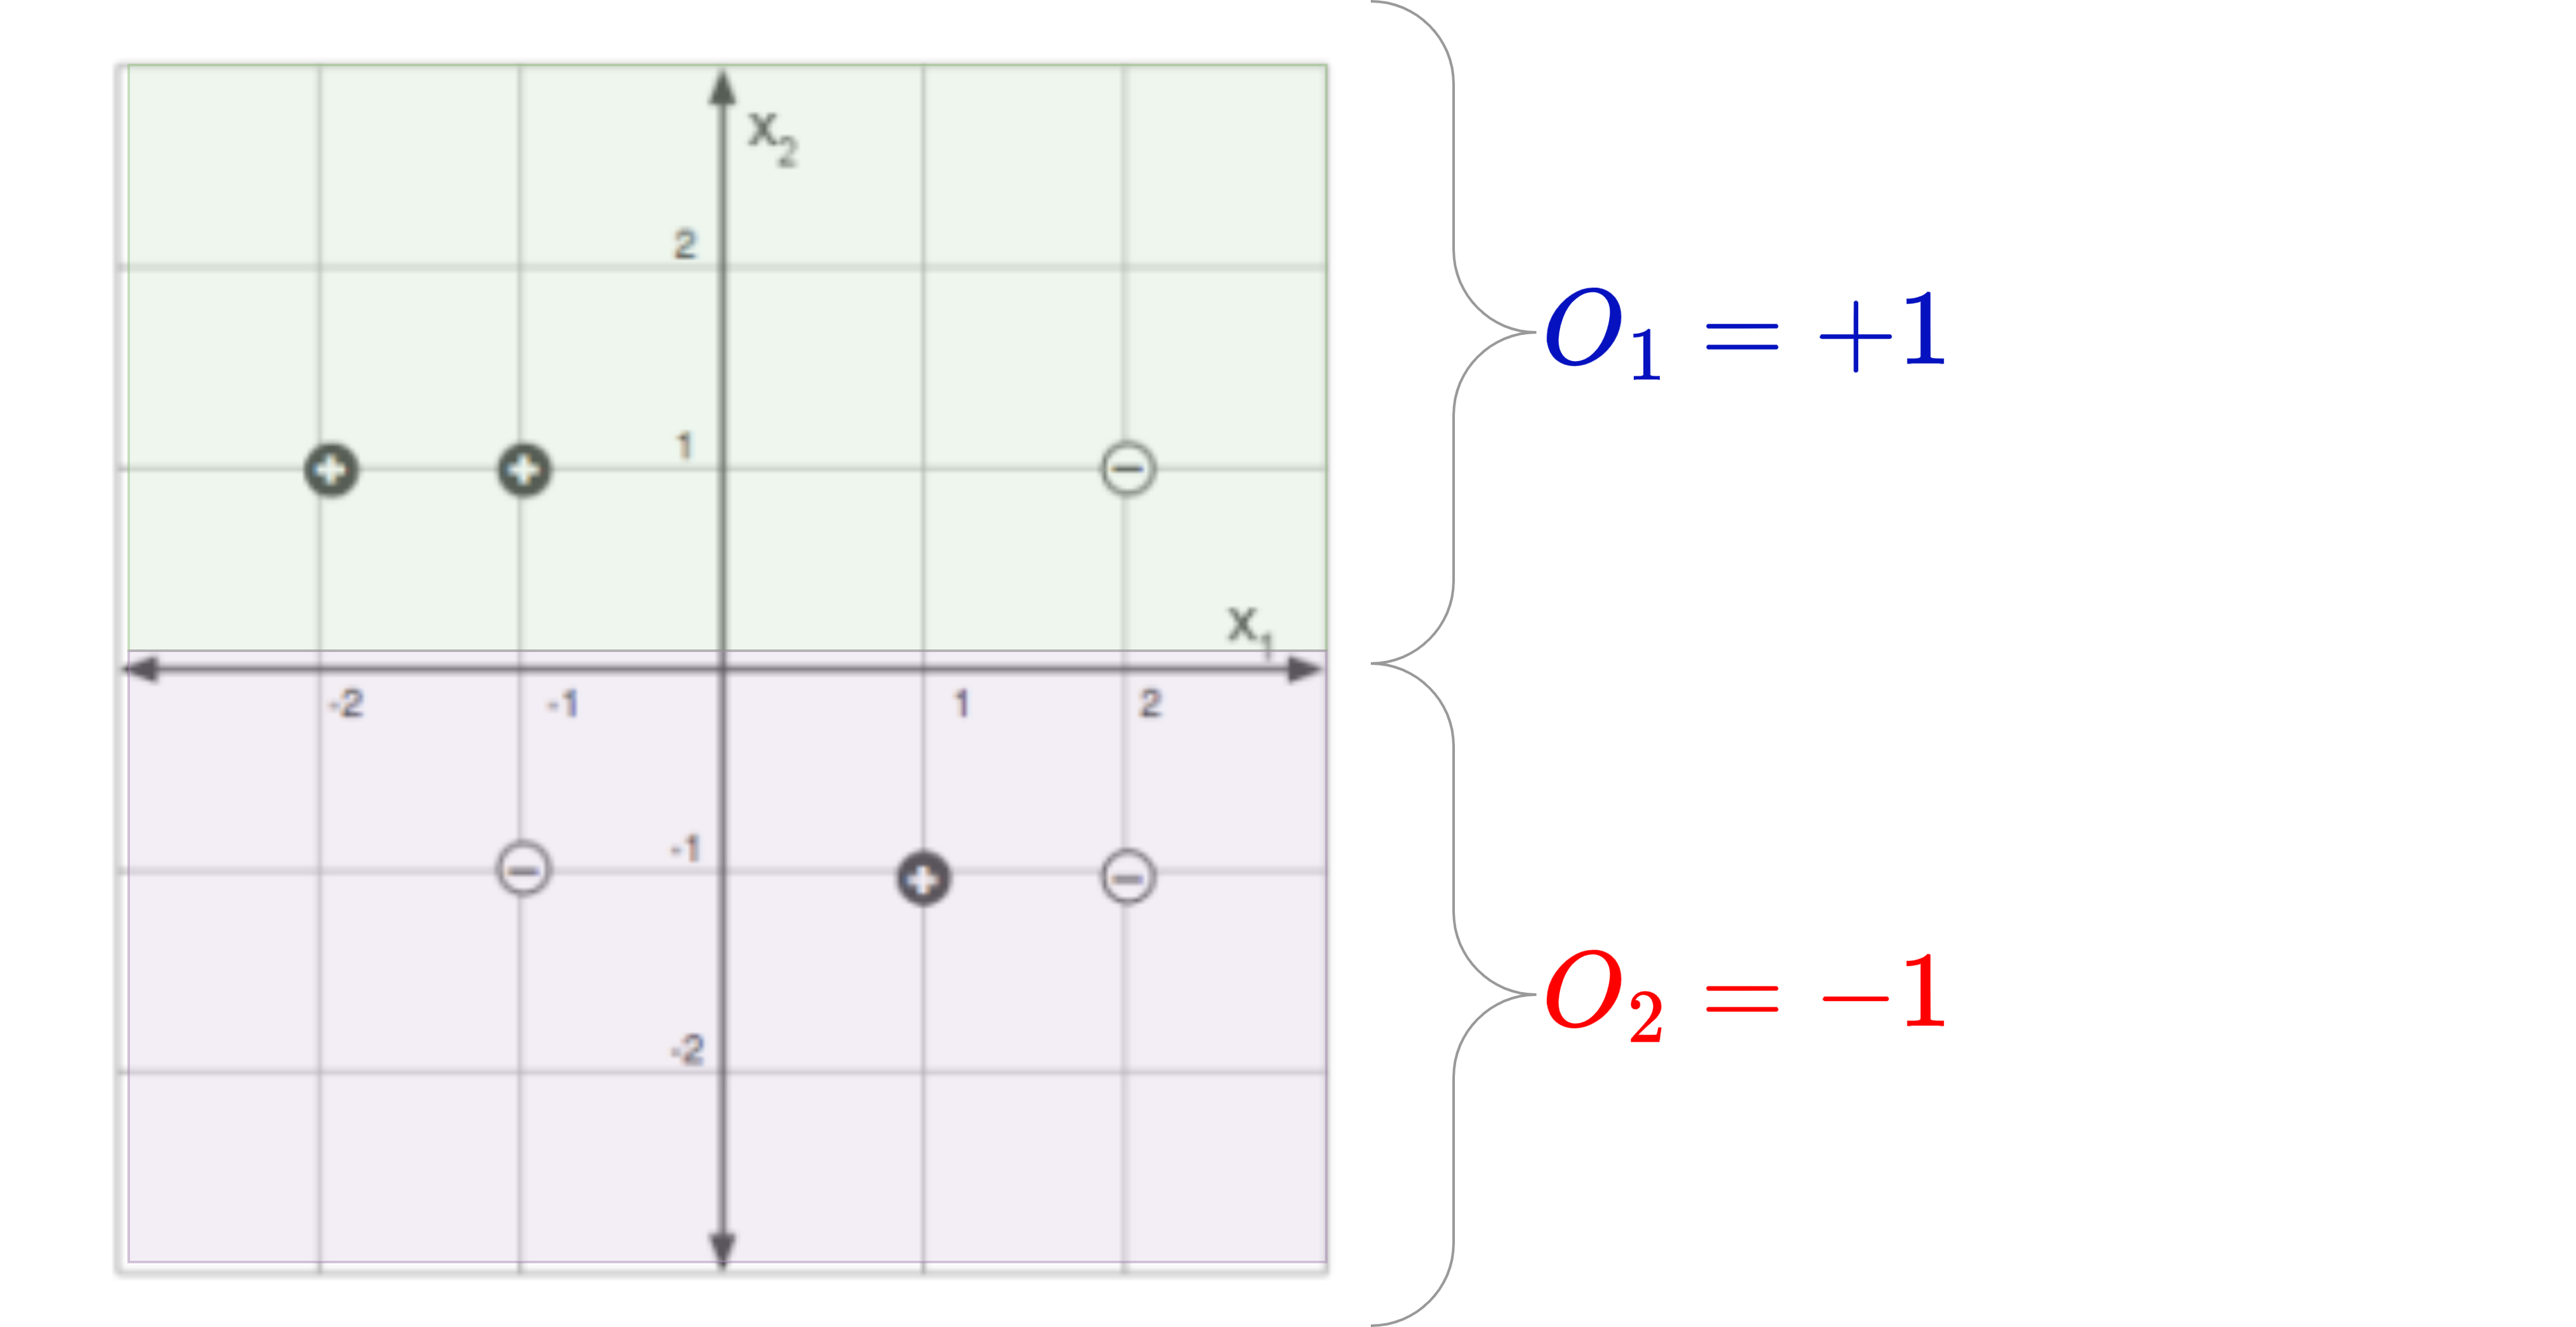
\includegraphics[width=90mm,scale=0.5]{images/nonparametric_images/x2_split_majority.png}
            \caption*{We create a split at $x_2=0$. For each region, we choose the most common class.}
        \end{figure}


    \phantom{}


    \subsection{Classification Loss: Misclassification Error}

        How do we measure our performance? 
        
        \begin{itemize}
            \item We'll need this kind of tool for choosing the \gren{best split}, \purp{pruning}, and \orgg{evaluating} our tree.
        \end{itemize}
        
        The simplest way would be, to simply count how many data points are misclassified.\\

        \begin{kequation}
            One way to measure loss of our classification tree in \orgg{region $m$} is \vocab{misclassification error}: the fraction of data points misclassified.

            \begin{equation*}
                Q_m(T) = \frac{\#\big( \text{Incorrectly Labelled, \orgg{region $m$}} \big)}
                {\#\big(\text{All data points, \orgg{region $m$}}\big)}
            \end{equation*}

            $Q_m(T)$ can also be seen as a \purp{probability}: if you pull a random data point, what's the chance that it was predicted incorrectly?
        \end{kequation}

        This is a pretty simple metric, but there's something else we can try.\\

    \subsection{"Purity" of child nodes: Empirical Probability}

        One possible problem with "misclassification error" is that it could be \gren{too simple}.

        \begin{itemize}
            \item \miniex Suppose that we have 6 different classes, and one of our regions has a 60\% accuracy rate.
            
            \item Our "incorrect" data points could be from \purp{5 different classes}. 
        \end{itemize}

        \begin{figure}[H]
            \centering
            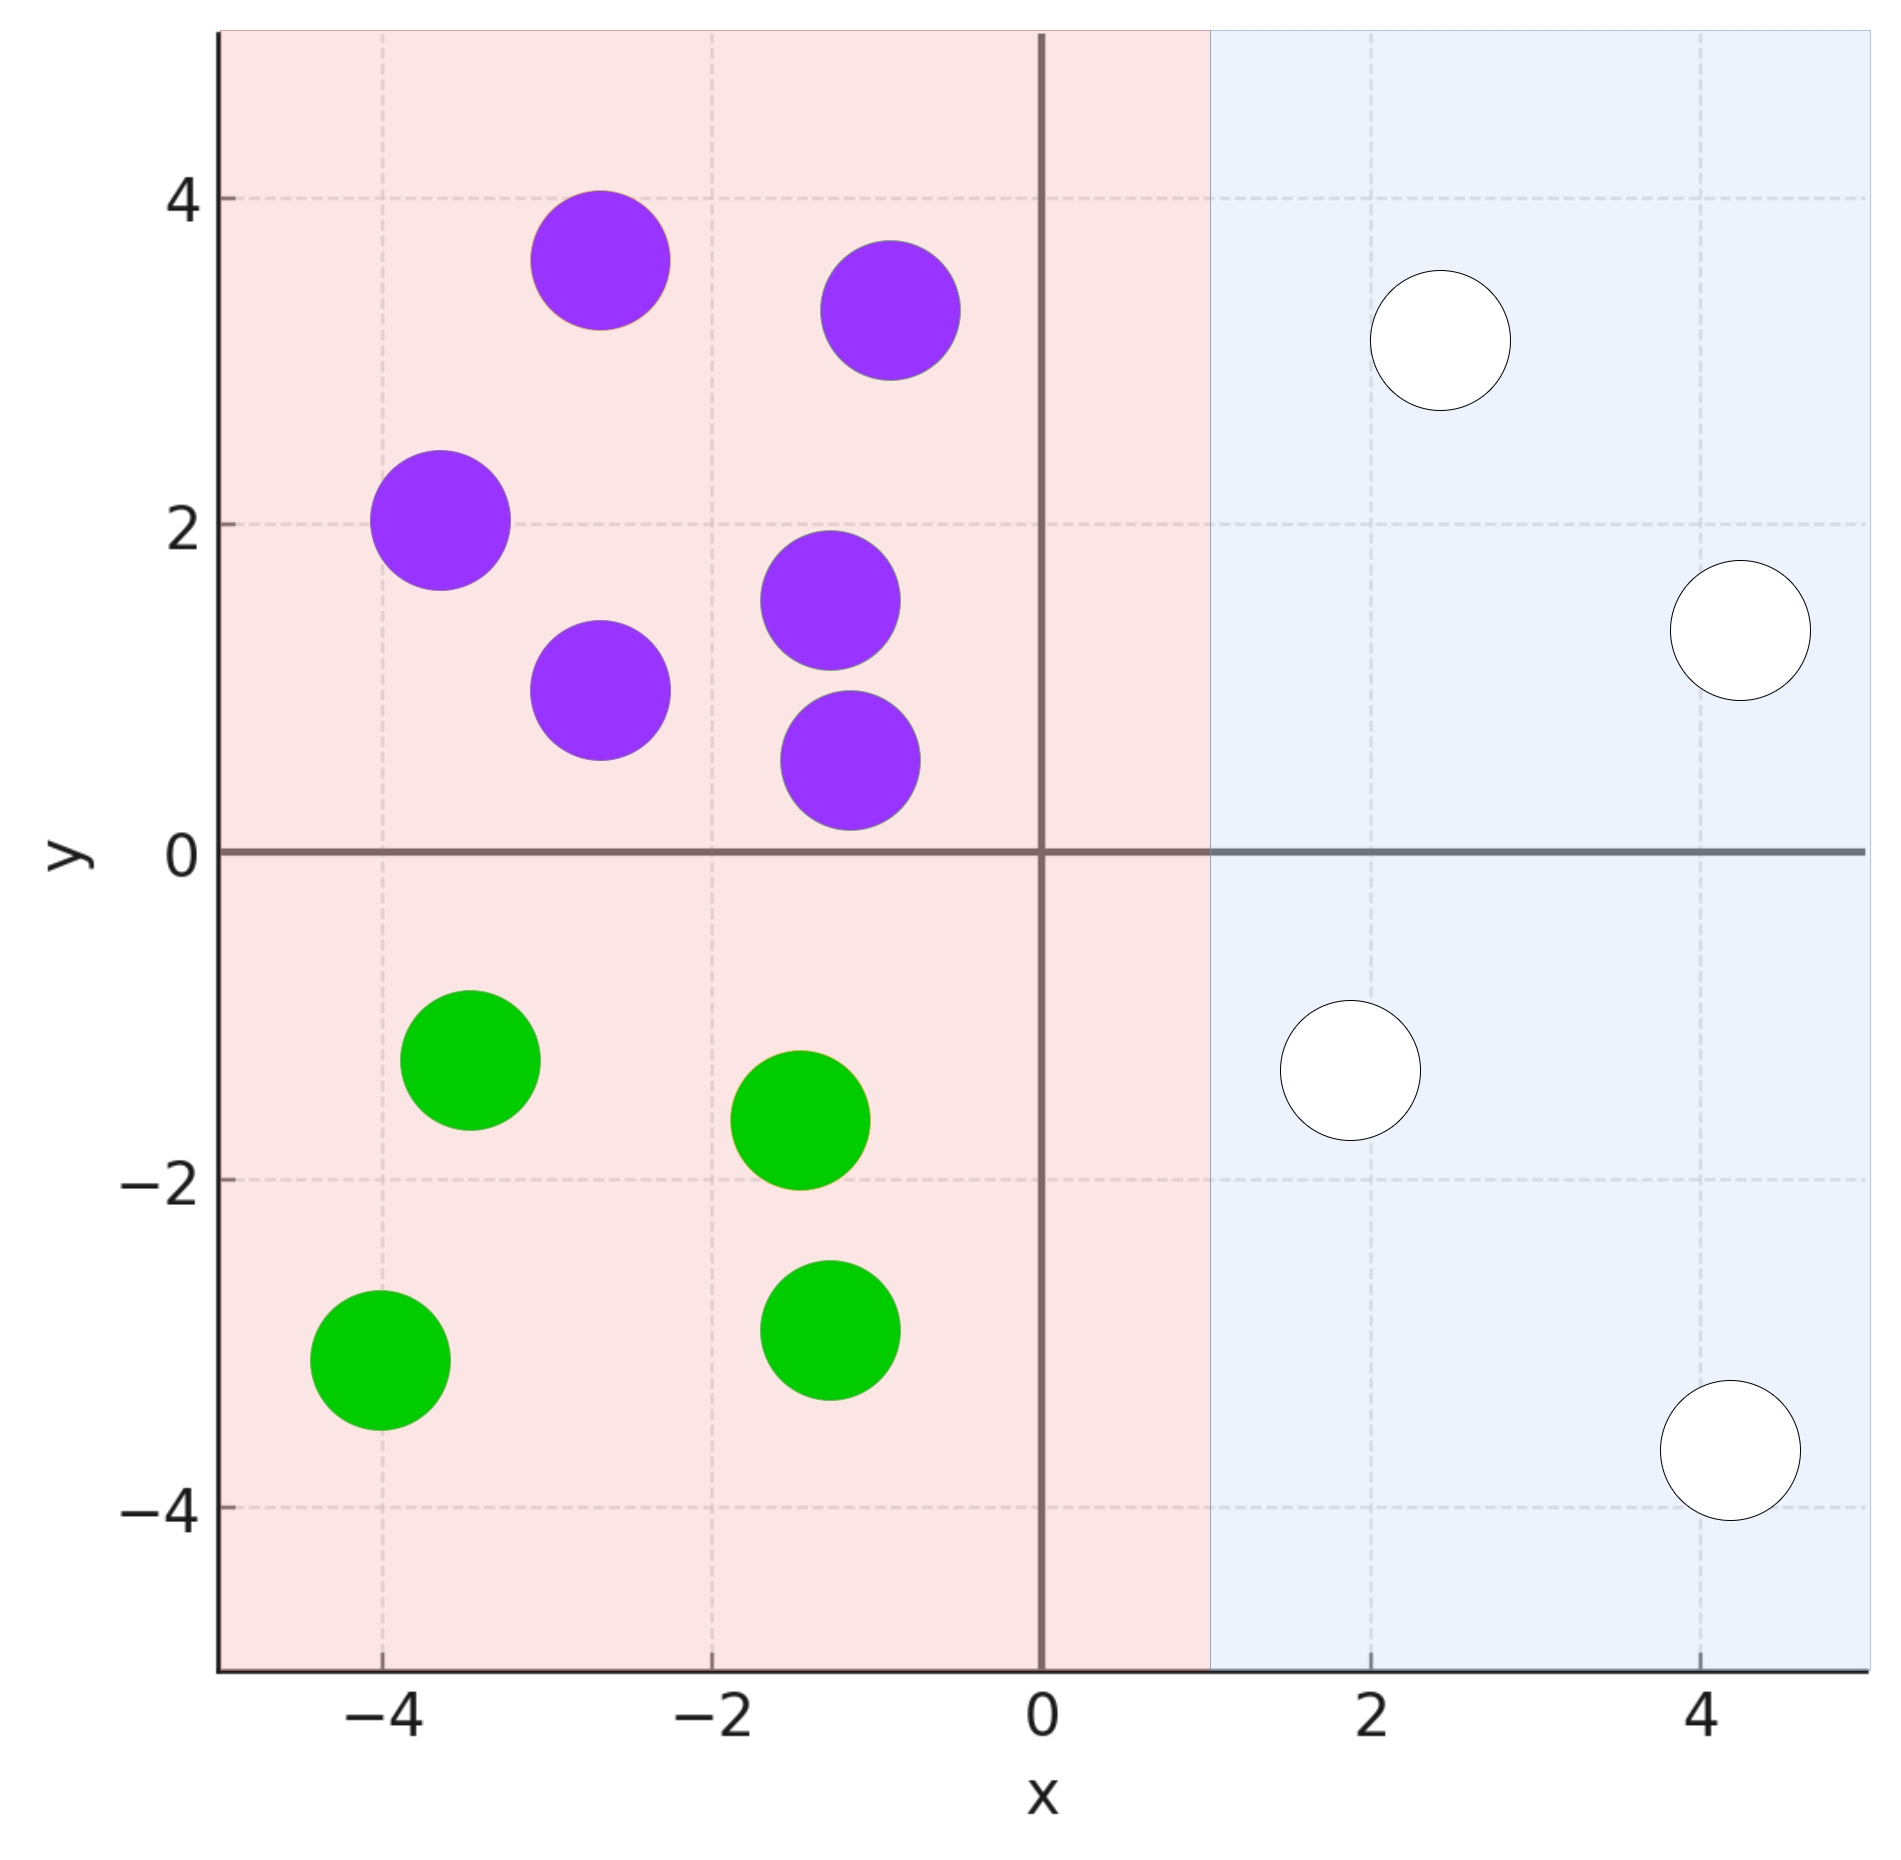
\includegraphics[width=50mm,scale=0.5]{images/nonparametric_images/pure_split.png}
            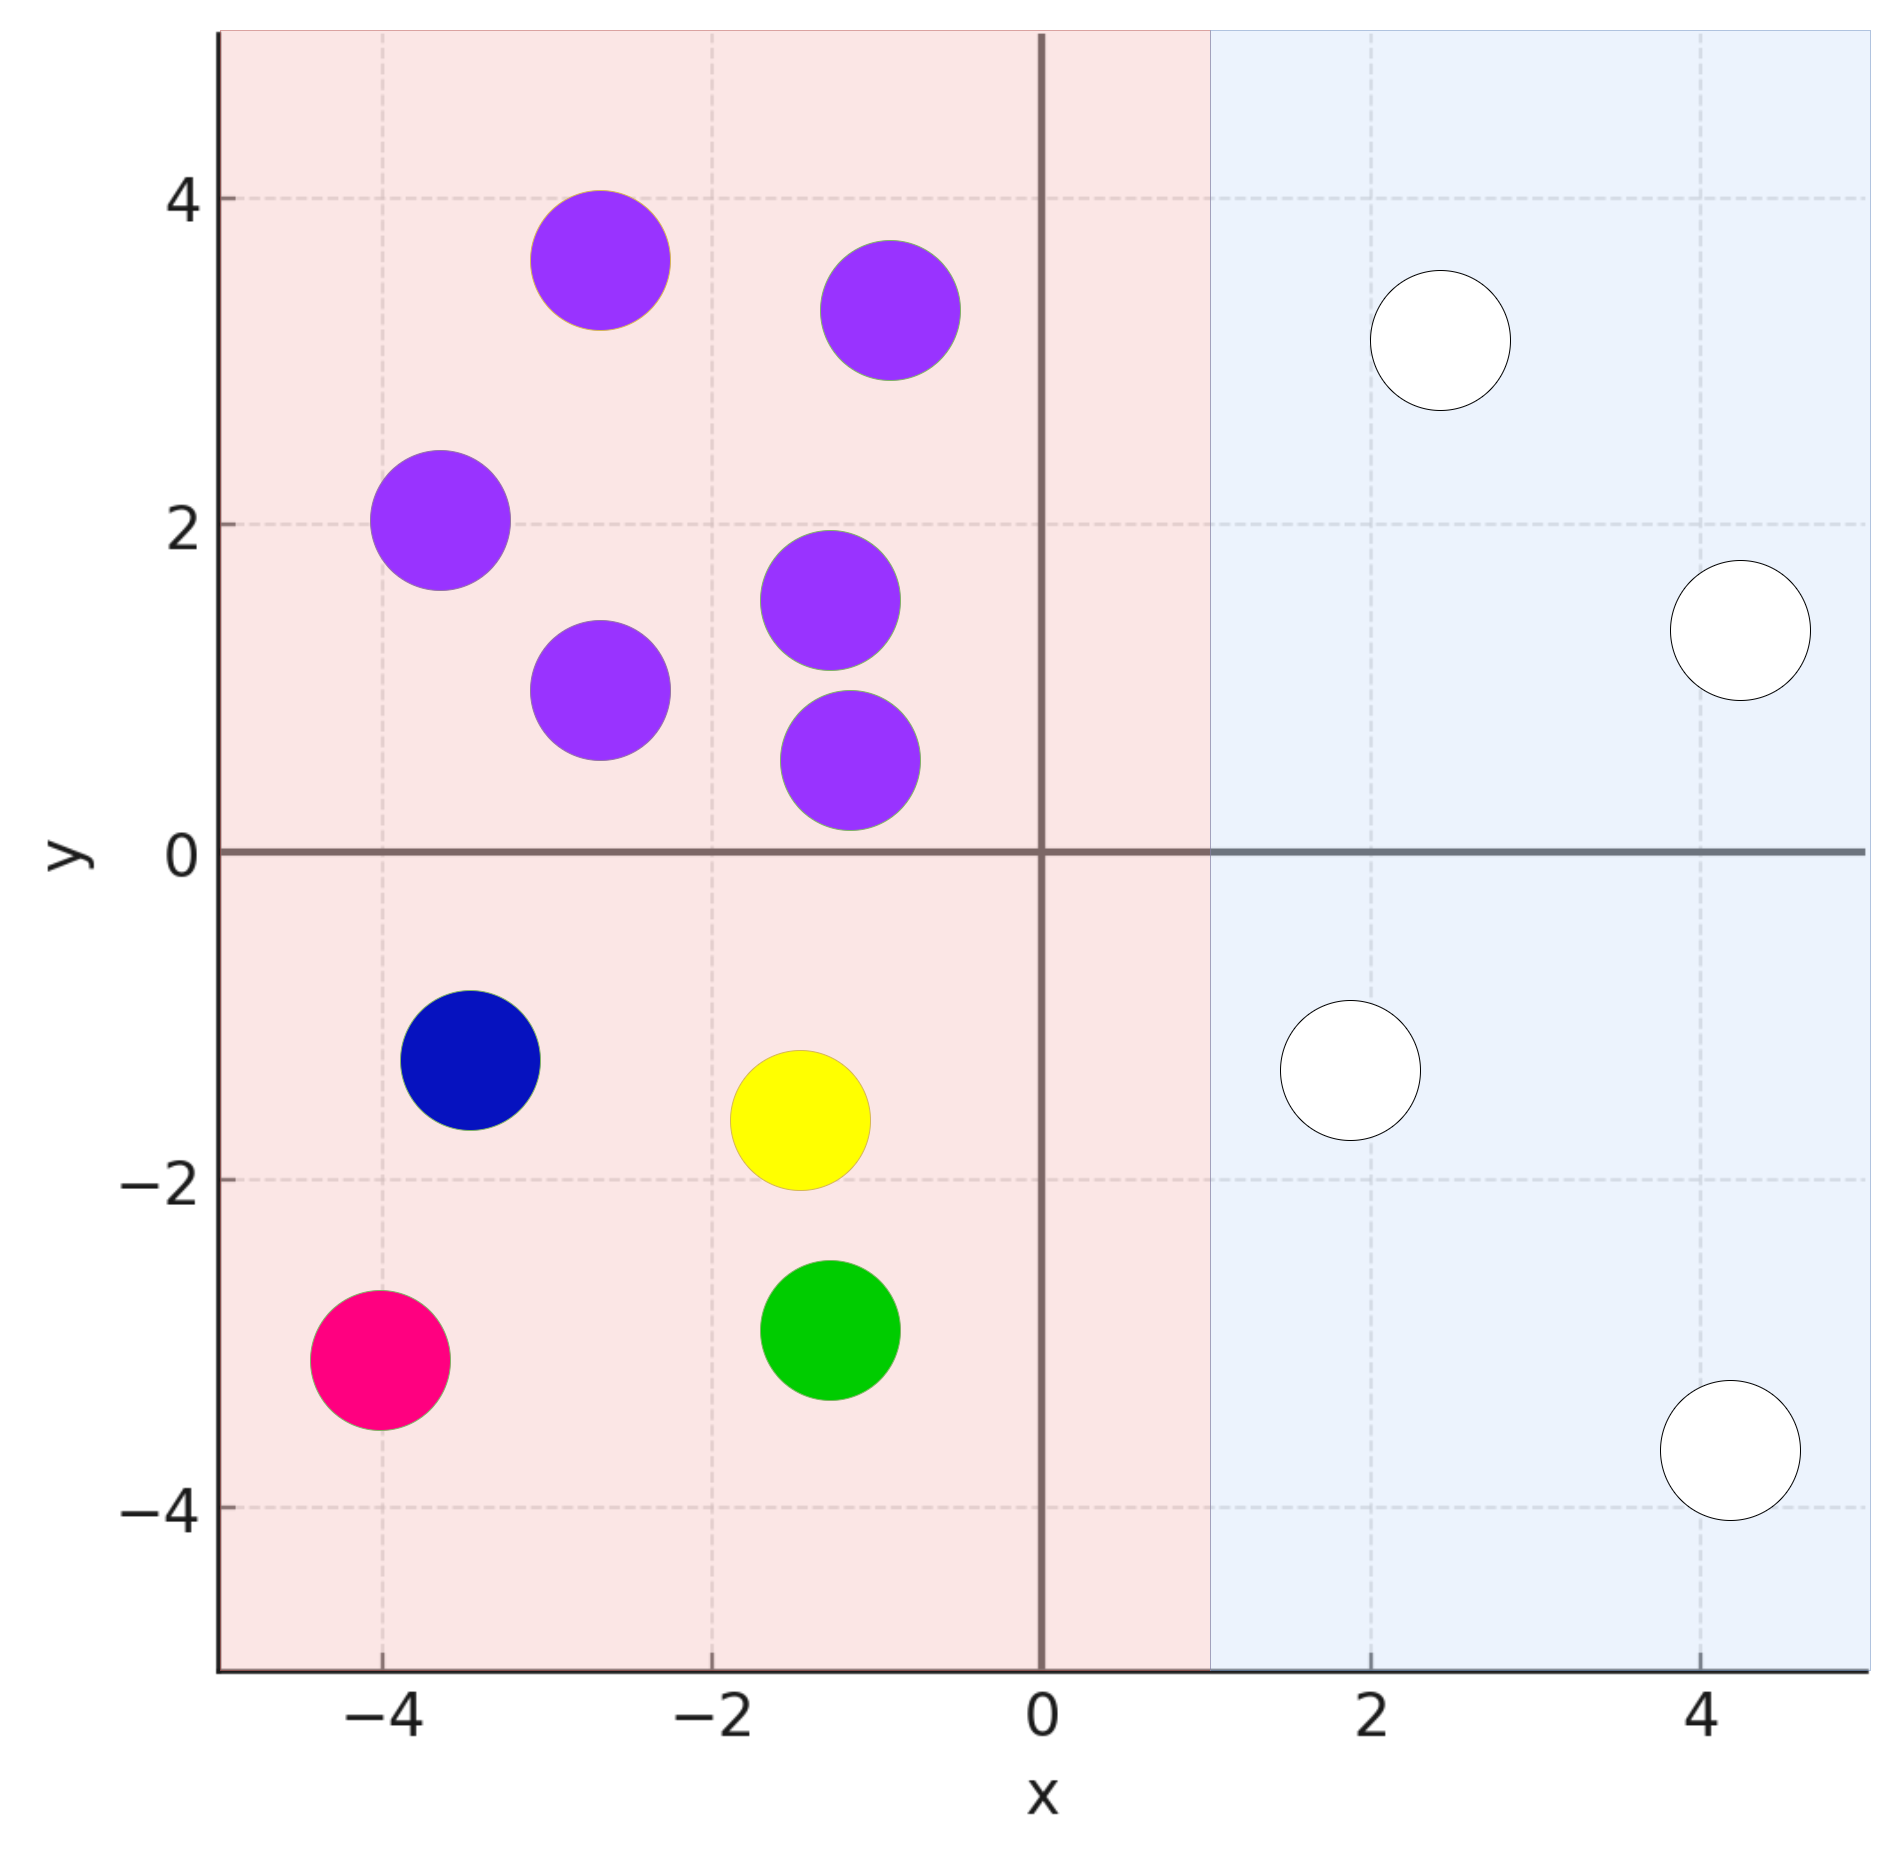
\includegraphics[width=50mm,scale=0.5]{images/nonparametric_images/impure_split.png}
            \caption*{Let's focus on the left region. These are two very different situations!}
        \end{figure}

        For our more "pure" split on the left, we get \orgg{perfect accuracy} with only one more split:
            \note{This is an exaggerated, "lucky" example: having more of the same category just makes it \purp{more likely} that we can find a good split.}

        \begin{figure}[H]
            \centering
            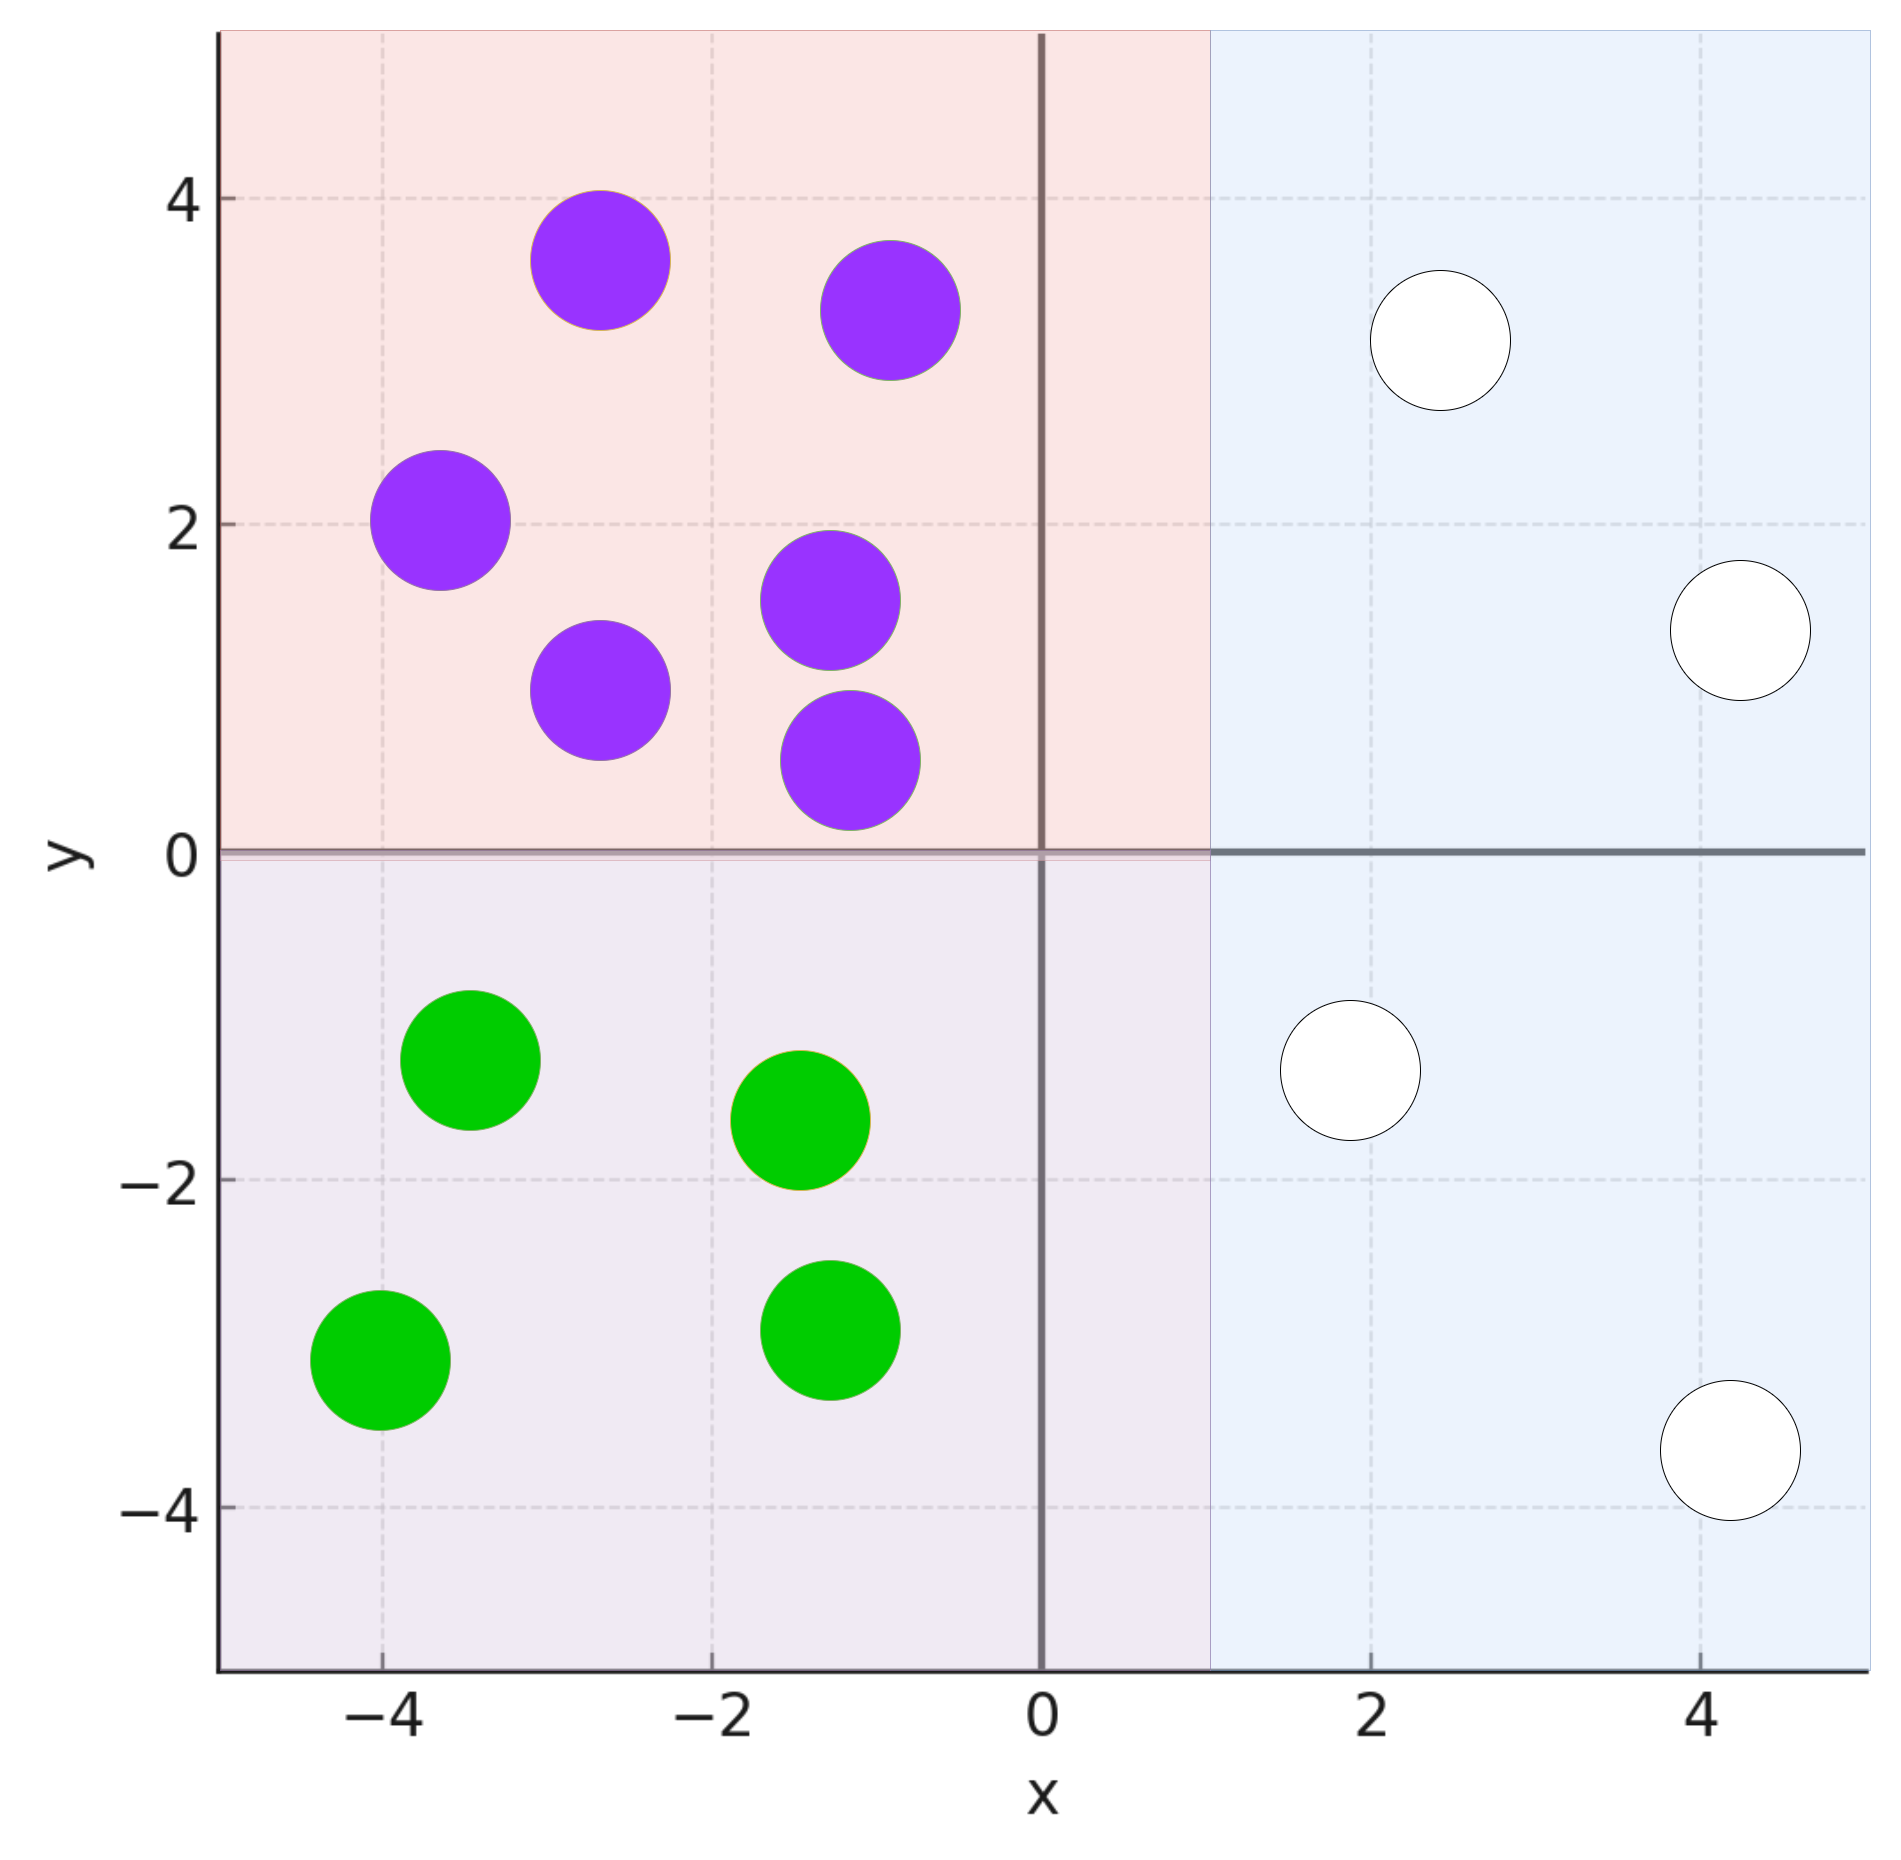
\includegraphics[width=50mm,scale=0.5]{images/nonparametric_images/perfect_split.png}
        \end{figure}

        While, this isn't true for the more "impure" split, with four different categories in the bottom-left.

        \begin{itemize}
            \item We can see that, despite having the same accuracy, the left split is generally "better".\\
        \end{itemize}

        \begin{concept}
            Our \vocab{tree classification} problem is generally \textit{easier} if our data is more \purp{concentrated}, in fewer categories. 

            \begin{itemize}
                \item If there are \gren{fewer} categories, it'll be easier to find a large group of data points in the \purp{same category}, to split from the rest.
            \end{itemize}

            So, we don't just prefer splits that have higher accuracy: we also prefer ones that create \orgg{more pure} regions ("child nodes").
        \end{concept}

        So, we want to measure how "pure" a region is.

        \begin{itemize}
            \item A region that is more pure will have a \gren{larger percentage} of data points in the same category.

            \item So, we want to measure the \textit{fraction} of our data from a given category.\\
        \end{itemize}

        \begin{definition}
            The \vocab{empirical probability} $\widehat{P}_{\org{m},\bro{k}}$ tells us what fraction of data points in \orgg{region $m$}, are in \brow{category $k$}.

            \begin{equation*}
                \widehat{P}_{\org{m},\bro{k}} =
                \frac{\#\big( \text{\brow{Category $k$}, \orgg{region $m$}} \big)}
                {\# \big( \orgg{\text{Region $m$}} \big)}
            \end{equation*}

            \begin{itemize}
                \item We call it "empirical probability", because we have the \purp{probability} of getting a data point in category $k$, in region $m$.
            \end{itemize}

            High $\widehat{P}_{\org{m},\bro{k}}$ means that \brow{category $k$} is very \gren{common} in \orgg{region $m$}.

        \end{definition}



        

    \subsection{Classification Loss 2: The Gini Index}

        Generally, we want a \gren{high} empirical probability in a few categories: that'll mean that \gren{most} of our data is in those few categories.
            \note{Naturally, this means low empirical probability in all the other categories.}

        \begin{itemize}
            \item We have \orgg{two} different metrics for measuring this property, of having our data "\purp{concentrated}" in a few categories.
            \item These are loss functions, so if they're large, then we have very "\purp{diluted}" data, with lots of categories.\\
        \end{itemize}

        \begin{concept}
            For our data to have high \vocab{purity}, we want our \purp{empirical probabilities} $\widehat{P}_{\org{m},\bro{k}}$ to all be either high, or low.

            \begin{itemize}
                \item In other words: a \gren{few} classes have a lot of data, \purp{the rest} have very little.

                \item The fewer the number of "popular" classes, the \orgg{more pure}.
            \end{itemize}
        \end{concept}

        Our first measure asks the question, "if we randomly select a data point, and then select \purp{another} (with replacement), what's the chance that we get a \gren{different class} the second time"?
            \note{"With replacement" means that it's possible the select the same data point twice: after we select the data point the first time, we don't remove it.}

        \begin{itemize}
            \item If we're likely to get a different category, each time we select one, that suggests that our data is "spread out" across a several categories.
                \note{Conversely, if our data was only in one class, then you'd always get the same category, every time.}
        \end{itemize}

        There are two (equivalent) expression that compute this.

        \begin{itemize}
            \item First version: we focus on the chance of them being the \gren{same} class.

                \begin{equation}
                    \prob{\text{2 different classes}} \quad=\quad 
                    1 - \prob{\text{Both same class}} 
                \end{equation}
        
                or,
        
                \begin{equation}
                    \overbrace{
                    Q_m(t) 
                    }^{\text{ \lblu{Region $m$}}}
                    \quad=\quad 1 - 
                    \overbrace{
                        \sum_{k} 
                        \underbrace{ \Big(\widehat{P}_{\org{m},\bro{k}} \Big)^2}
                        _{\text{ \lblu{Same class twice} }}
                    }^{\text{ \lblu{Sum over all classes} }}
                \end{equation}
        
            \item Second version: We select a first class $k$, and then, make sure our second class is \purp{different}.


                \begin{equation}
                    \prob{\text{2 different classes}} \quad=\quad 
                    \sum_k \prob{\text{Class $k$}} \cdot  \prob{\text{Not class $k$}}
                \end{equation}


                or,

                \begin{equation}
                    \overbrace{
                    Q_m(t) 
                    }^{\text{ \lblu{Region $m$}}}
                    \quad=\quad 
                    \overbrace{
                        \sum_{k} 
                        \underbrace{ \Big(\widehat{P}_{\org{m},\bro{k}} \Big) \cdot \Big( 1-\widehat{P}_{\org{m},\bro{k}} \Big)}
                        _{\text{ \lblu{Class $k$, then different class} }}
                    }^{\text{ \lblu{Sum over all classes} }}
                \end{equation}
        \end{itemize}

        \begin{kequation}
            Another way to measure the loss of our split is the \vocab{Gini index}:

            \begin{itemize}
                \item "If we randomly sample \orgg{two} data points (with replacement), what's the probability they have \purp{different classes}?"
            \end{itemize}

            \begin{equation*}
                Q_m(t) 
                \qquad=\qquad 
                    \sum_{k}  \Big(\widehat{P}_{\org{m},\bro{k}} \Big) \cdot \Big( 1-\widehat{P}_{\org{m},\bro{k}} \Big)
                \qquad=\qquad 
                1-\sum_{k} 
                \Big(\widehat{P}_{\org{m},\bro{k}} \Big)^2
            \end{equation*}
        \end{kequation}

        \phantom{}

        


    \subsection{Information 1: Uncertainty (\redd{Optional})}
    
        Entropy is another measure we can use. Entropy comes from \purp{information theory}: we want each of our splits to give us the \gren{most} information possible.

        \begin{itemize}
            \item But what do we mean by "information"?

            \item Let's consider our very "\orgg{informative}" tree example from the beginning of this section:
        \end{itemize}

        \begin{figure}[H]
            \centering
            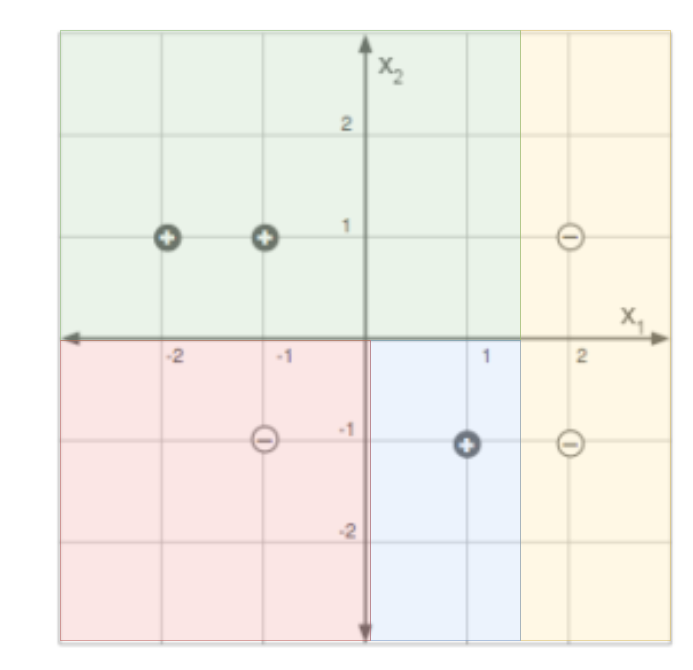
\includegraphics[width=50mm,scale=0.5]{images/nonparametric_images/full_tree.png}
            \caption*{Based on which region you're in, you know the exact class of your data.}
        \end{figure}

        The tree provides perfect information, for \purp{classifying} the training data: if we know the region of our data point, we know its classification.
        
        \begin{itemize}
            \item In other words, we have \gren{no uncertainty} left.\\
        \end{itemize}

        \begin{definition}
            \vocab{Uncertainty} describes "how much" randomness we have in our outcome. 

            The more information we gain, the \gren{less uncertainty} remains. 
        \end{definition}
        
        This is the kind of information we're discussing.

        \begin{itemize}
            \item Let's investigate further: what does "incomplete" information look like? 
        \end{itemize}


        \begin{figure}[H]
            \centering
            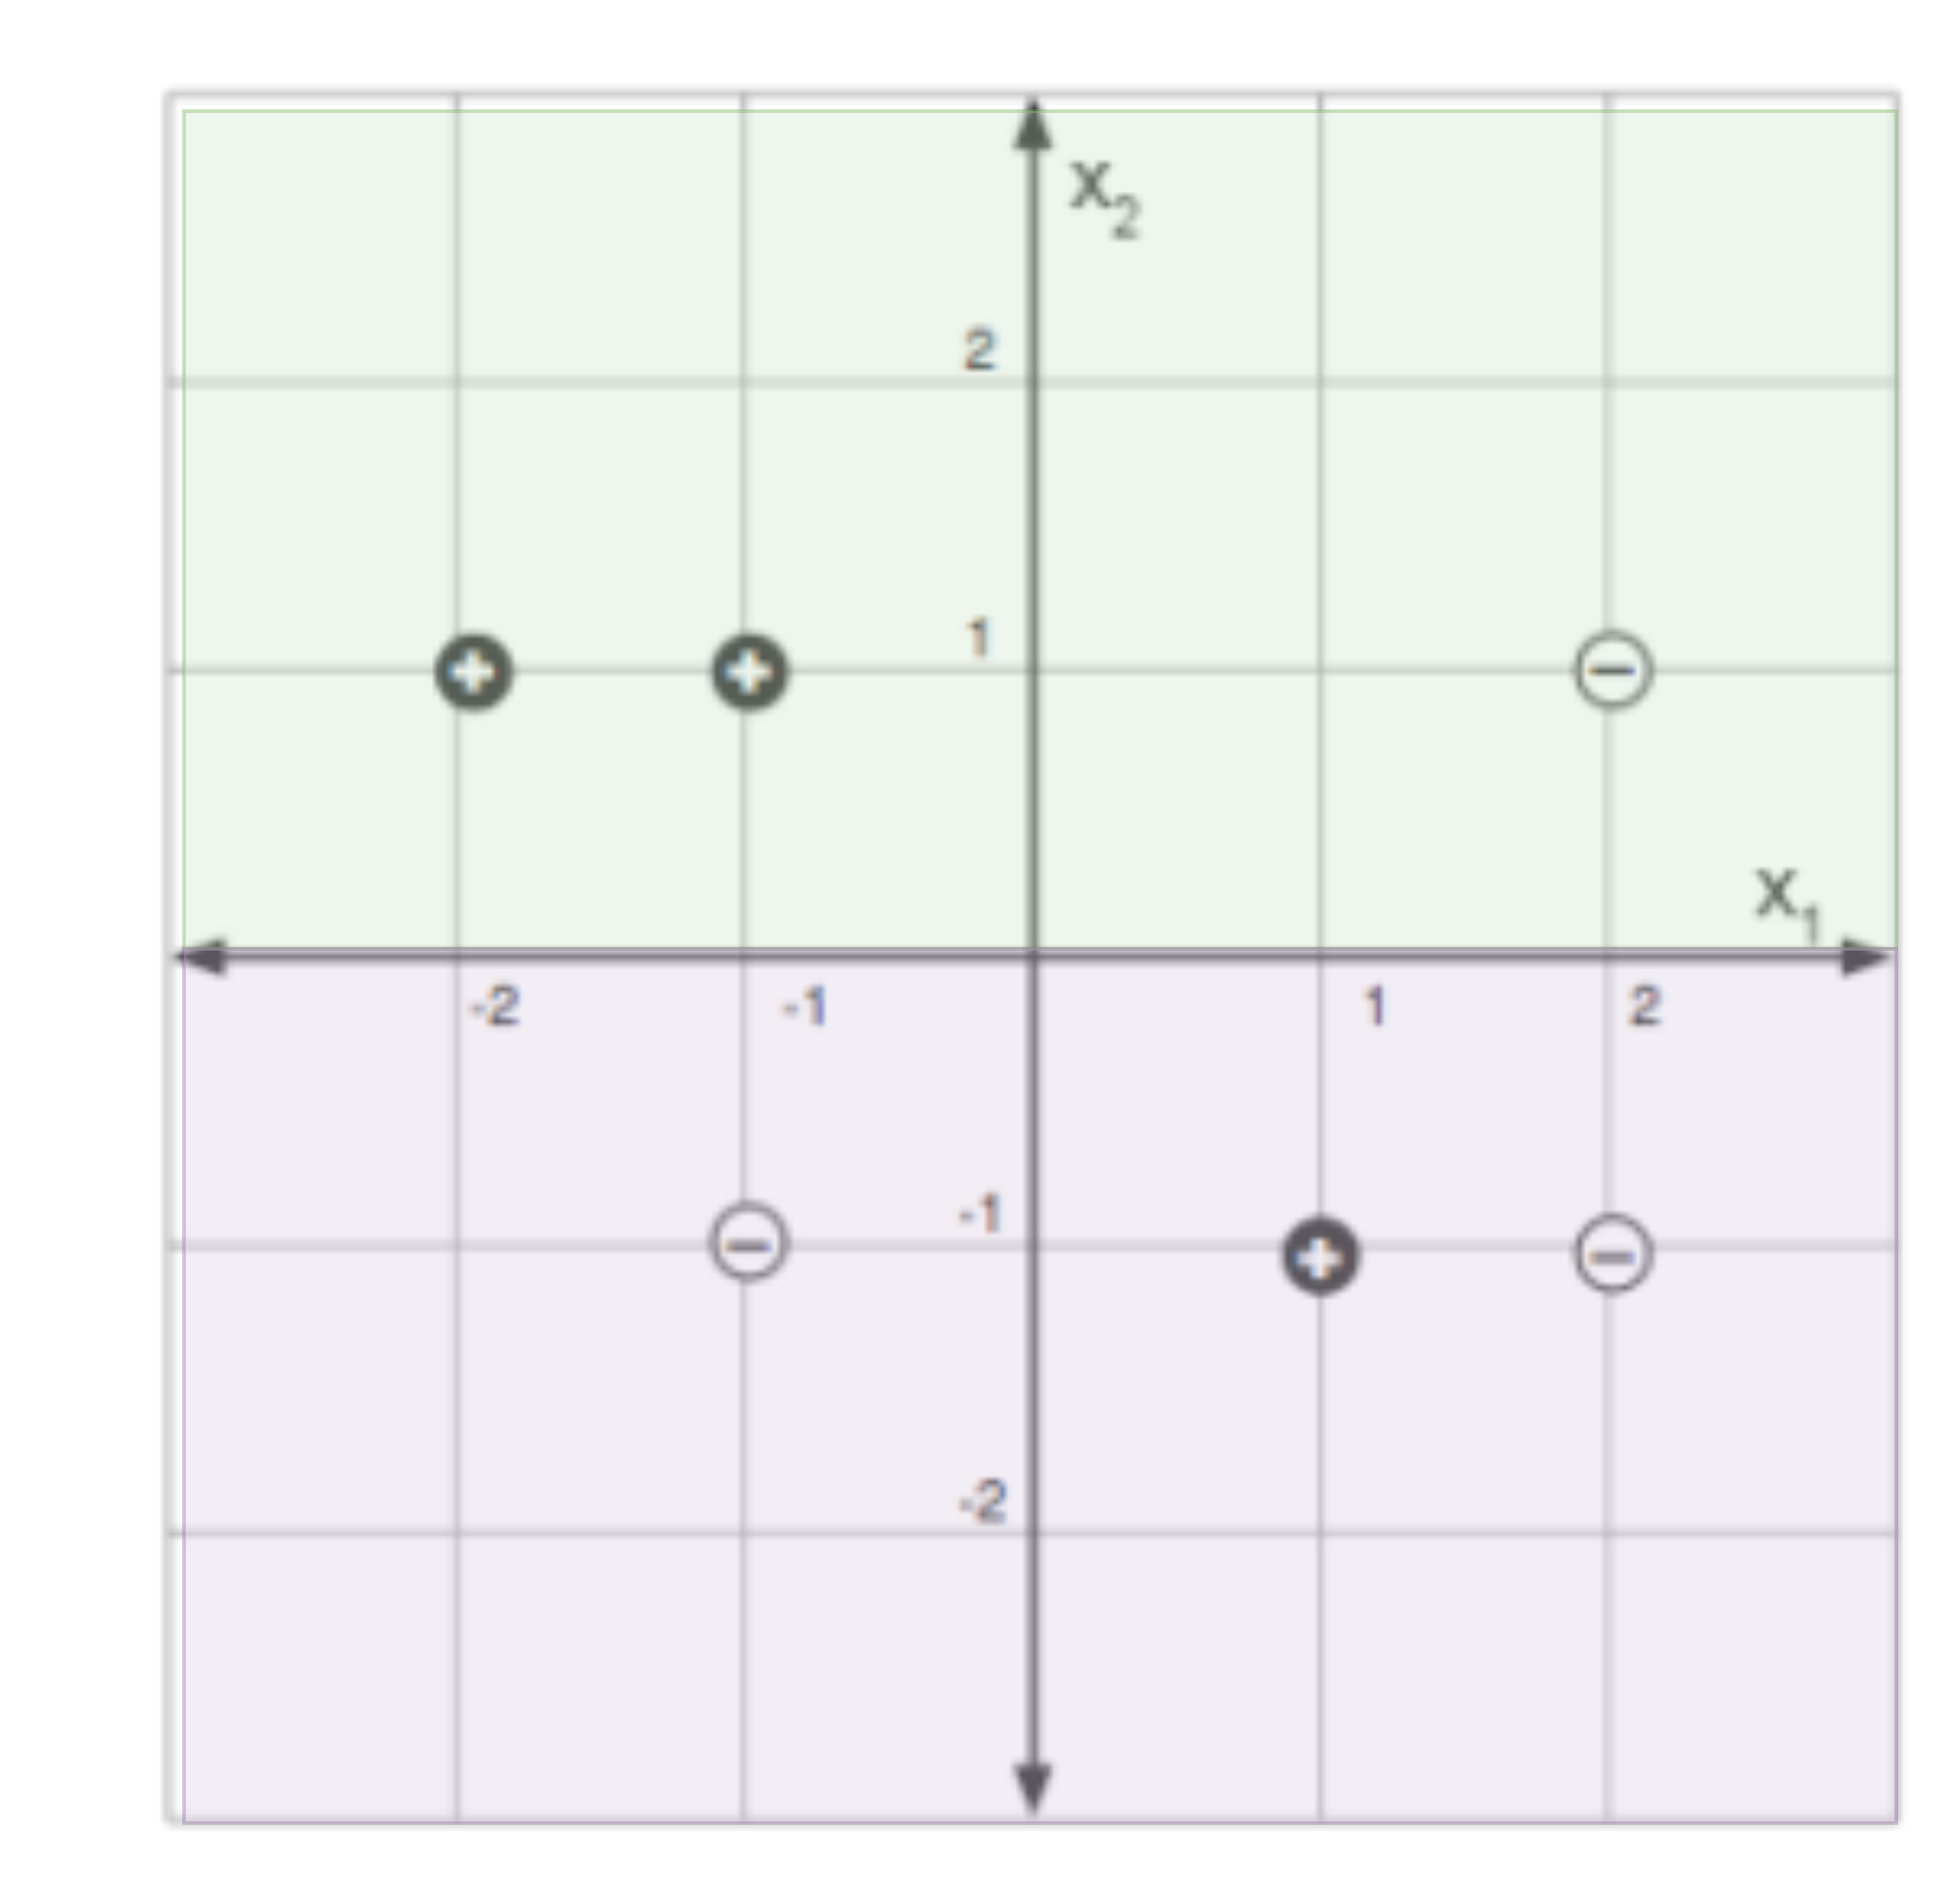
\includegraphics[width=50mm,scale=0.5]{images/nonparametric_images/x2_split.png}
            \caption*{Even if we know the region we're in, we're still uncertain about the classification of our data.}
        \end{figure}

        This tree is less "informative", because we \purp{don't know} exactly what class we're in. 

        \begin{itemize}
            \item Still, it's better than no splits: in the top half, we have more +1 data than -1: we have \gren{less uncertainty} than before.
                \note{If you had to guess the classification, and you guessed +1, you'd be right 2/3 of the time, rather than half the time.}\\
        \end{itemize}

        \begin{concept}
            Our tree is designed to provide \purp{information} about our data:

            \begin{itemize}
                \item If you learn that a data point is in region $R_m$, you are \orgg{more certain} in guessing which class it's in.
            \end{itemize}

            The \gren{less variation} we have in a region, the more \textbf{informative} it is: 

            \begin{itemize}
                \item If a region $R_m$ only contained a \purp{single class}, you would know \textbf{exactly} the class of any data point you find there.
                \item But if there are many classes that are all likely, then you're pretty \vocab{uncertain} about which class to choose.
            \end{itemize}
        \end{concept}

        \miniex You want to figure out if someone is sick. If I say, "she yawned earlier", that doesn't help: plenty of people (sick and non-sick yawn.

        \begin{itemize}
            \item But, if I say, "she's sneezing and coughing", that narrows things down: a lot more people who are sneezing and coughing, are sick.
        \end{itemize}

    \phantom{}

    \subsection{Information 2: Entropy (\redd{Optional})}

        Now, we have an idea of what we want. Next, we need to figure out how to \orgg{quantify} information.

        \begin{itemize}
            \item Let's use \purp{complete certainty} as a baseline: the situation where we know exactly what class we're in.

            \item How much more work do we need to do, before we know our class with \gren{100\% confidence}?\\
        \end{itemize}

        \begin{concept}
            Our goal is to measure our "\purp{distance}" from being \gren{completely certain} in our classification.
        \end{concept}

        Suppose we want to identify a random data point. We use our \orgg{tree structure} to narrow it down to $R_m$. We've gained some information. 

        But how far are we from \vocab{complete certainty}?


        \begin{itemize}
            \item Our binary tree recursively split our data into two parts, so that we could "\gren{narrow down}" our classification. 

            \item We'll re-use that idea here: we'll ask a \purp{binary} yes-or-no question, to narrow it down further. 
        \end{itemize}
        
        
        We'll assume the \orgg{best case}:\\

        \begin{concept}
            We'll \vocab{measure uncertainty} based on how many \gren{binary questions} we have to ask about our data point, before we're completely certain of its class:

            \begin{itemize}
                \item Each binary question eliminates \purp{half} of the data.
                \item We're careful with our split: we only remove data that is from a \gren{different class} from our true data.
            \end{itemize}

            In other words: "how much work (how many questions) do you need to do, to get complete certainty?"

            \begin{itemize}
                \item If it takes more work, you're \orgg{more uncertain} of your answer.
            \end{itemize}
        \end{concept}

        \miniex We select a data point, which happens to be in class $A$. Class $A$ makes up \org{1/8} of the data.

        \begin{itemize}
            \item First question: we've remove half, Class $A$ is \org{1/4} of the remaining data.
            \item Second question: we remove half again, Class $A$ is \org{1/2}.
            \item After 3 questions, \org{all} of our data is class $A$: our data point must be in class $A$.
        \end{itemize}

        \begin{figure}[H]
            \centering
            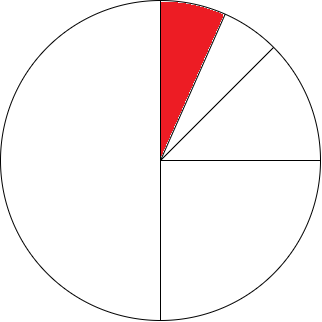
\includegraphics[width=30mm,scale=0.5]{images/nonparametric_images/dataset_split.png}
            \caption*{We have to split our data in half 3 times, to get down to our 1/8.}
        \end{figure}

        So, each time, we \purp{double} the proportion of class $A$. 

        \begin{itemize}
            \item If $p=1/8$, then we double 3 times. If $p=1/16$, we double 4 times, and so on.

            \item This matches the behavior of the \gren{logarithm} with \orgg{base 2}.
                \note{This can be a bit weird when our probability isn't a power of 2: for example, 1/3. In which case, we could round up: we have to ask 2 questions.
                
                \phantom{}
                
                But when we're computing uncertainty, we still consider 1/4 "more uncertain" than 1/3. So, we'll allow non-integer values.}
        \end{itemize}

        \begin{equation}
            \log_2 \Bigg( \frac{1}{p_i} \Bigg) = - \log_2 (p)
        \end{equation}

        \begin{kequation}
            Each class $c_i$ contributes to the \vocab{uncertainty} within our region $R_m$: 

            \begin{equation*}
                \log_2 \Bigg( \frac{1}{p_i} \Bigg) = - \log_2 (p_i)
            \end{equation*}

            We also sometimes call this...

            \begin{itemize}
                \item \vocab{Information}: if you need to ask $n$ questions to narrow down your data, then you need $n$ binary answers: $n$ \purp{bits of information}.

                \item \vocab{Surprisal}: if an outcome is less common/likely (lower $p$), then we're \gren{more surprised} when it happens.
            \end{itemize}
        \end{kequation}

        But we're not quite done: this is just our uncertainty associated with one of our outcomes.

        \begin{itemize}
            \item How do we aggregate this, over all of our possible classes?
        \end{itemize}

        We'll get the \orgg{expected value}: if we pull a random data point, what's the \purp{average number} of \gren{binary questions} until we've identified it?

        \begin{equation}
            E[X] = \sum_i p(x_i) \cdot x_i \quad \implies \quad 
            - \sum_i p_i \log_2 (p_i)
        \end{equation}

        This is called \vocab{Entropy}.\\

        \begin{definition}
            \vocab{Entropy} $H(X)$ tells us how \purp{spread-out} our data is, across different outcomes.

            \begin{itemize}
                \item More entropy means that our data is more spread-out, and \gren{uncertain}.
            \end{itemize}

            \begin{equation*}
                H(X) \quad=\quad - \sum_i p_i \log_2 (p_i)
            \end{equation*}

            \subsecdiv

            In the simplified case, we could think of this as answering the following question:

            \begin{itemize}
                \item If we pull a random data point, what's the \purp{average number} of \gren{binary questions} until we've identified it?
            \end{itemize}
        \end{definition}    

        What do we do if we have a non-integer entropy? This still measures how "spread-out" or uncertain our data is: 
        
        \begin{itemize}
            \item We're closer/further from having to add one more binary question.
        \end{itemize}



    \phantom{}

    \subsection{Classification Loss 3: Entropy}

        Now, we move back to our tree. We need to make one notational change: \textit{empirical probability}.\\

        \begin{kequation}
            The entropy of a \gren{region} is computed with our \purp{empirical probabilities}:

            \begin{equation*}
                H(I_m) \quad=\quad - \sum_i 
                \widehat{P}_{\org{m},\bro{k}} \cdot
                \log_2 \Big( \widehat{P}_{\org{m},\bro{k}} \Big)
            \end{equation*}

            This is one way to measure the \orgg{purity} of our data.
            
        \end{kequation}

        One important caveat:\\

        \begin{clarification}
            $0\log_2(0)$ is \vocab{not defined}. However, for calculations, we usually assume:

            \begin{equation*}
                0\log_2(0) = 0
            \end{equation*}

            \begin{itemize}
                \item The \gren{limit} supports this choice:

                \begin{equation*}
                    \lim_{n \to 0} n \log_2(n)  = 0
                \end{equation*}

                \item Additionally, we use entropy to indicate "\orgg{uncertainty}". With no data, there's no uncertainty.
            \end{itemize}
        \end{clarification}

        Now that we have entropy, we can use it to determine the best splits.

        \begin{itemize}
            \item The lower the entropy, the less \gren{spread-out} our data is.

            \item So, we want splits that \purp{reduce entropy} the most.\\
        \end{itemize}

        \begin{concept}
            In our greedy algorithm, we choose the splits with the \purp{lowest entropy}:

            \begin{itemize}
                \item These are the splits which give us the most "\gren{information}" about our data.
            \end{itemize}

            \subsecdiv

            Because we have fewer classes in each region, our next split may give better accuracy, as well.
        \end{concept}

            \note{We discussed the possible benefits of having more "pure" data in 12.2.11. 
            
            \phantom{}
            
            A region with only 2 classes of data, might be more easily split, than a region with 5 classes.}

        How do we compute the "\gren{change} in entropy" after we've split? We could just add, or \textbf{average}, the entropy of both regions.

        \begin{itemize}
            \item But, this could be \purp{misleading}: if we split our data into a region of 2 data points, and a region of 20 data points, we probably care more about the region with 20.

            \item So, we'll do a \orgg{weighted average}: the region with more data points, contributes more to entropy.
        \end{itemize}

        \begin{equation}
            \frac{\# \text{(Data in region $m$)}}{\# \text{(Total data)}} \cdot \overbrace{H(I_m)}^{\text{Entropy in region}}
        \end{equation}

        Or, using more dense notation:
            \note{Remember that $I$ represents all of your data points, while $I_m$ represents data in a region.}

        \begin{equation}
            \Bigg( \frac{\# I_m}{\#I} \Bigg) \cdot \overbrace{H(I_m)}^{\text{Entropy in region}}
        \end{equation}

        \begin{kequation}
            The \vocab{entropy} $\widehat{H}$ \textit{after} a split is the \orgg{weighted average} of the two splits:

            \begin{equation*}
                \widehat{H} 
                \quad=\qquad 
                \Bigg(\frac{\#\red{I^+}}{\#I} \Bigg) \cdot H(\red{I^+}) 
                \quad+\quad 
                \Bigg(\frac{\#\blu{I^-}}{\#I} \Bigg) \cdot H(\blu{I^-})
            \end{equation*}

            Our data $I$ is broken into $I^+$ (data points above split), and $I^-$ (data points below the split).
        \end{kequation}

        If we want to be pedantic, we could create separate notation for splitting at value $s$, on axis $j$: we use $I_{j,s}$ notation.

        \begin{equation}
            \widehat{H} 
            \quad=\qquad 
            \Bigg(\frac{\#\red{I^+_{j,s}}}{\#I} \Bigg) \cdot H(\red{I^+_{j,s}}) 
            \quad+\quad 
            \Bigg(\frac{\#\blu{I^-_{j,s}}}{\#I} \Bigg) \cdot H(\blu{I^-_{j,s}})
        \end{equation}

        We can also say that we "\gren{gain information}" when we reduce entropy: it takes \purp{less} additional information to completely know our classification.\\

        \begin{kequation}
            The \vocab{information gained} from a split comes from comparing the entropy, before and after the split:

            \begin{equation*}
                \text{InfoGain} = \overbrace{H(I_m)}^{\text{Pre-split}} - \overbrace{\hat{H}}^{\text{Post-split}}
            \end{equation*}
        \end{kequation}


    \phantom{}

    \subsection{Which Loss function to use?}

        In the past, there's been a lot of debate over which loss function works best.

        \begin{figure}[H]
            \centering
            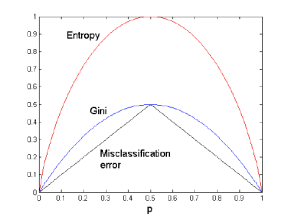
\includegraphics[width=50mm,scale=0.5]{images/nonparametric_images/classification_loss.png}
        \end{figure}

        All three capture the basic idea of accuracy/purity:

        \begin{itemize}
            \item If a class matches \purp{none} of our data ($\widehat{P}_{m,k}=0$), it doesn't contribute to the loss.
            \item If a class matches \gren{all} of our data ($\widehat{P}_{m,k}=1$), it \textit{also} doesn't contribute to the loss.
        \end{itemize}

        For our purposes, we'll consider the following.\\

        \begin{concept}
            Traditionally, we use:

            \begin{itemize}
                \item \purp{Entropy} for tree-builiding
                \item \gren{Misclassification error} for pruning
            \end{itemize}
        \end{concept}





    \pagebreak

    \subsection{Bagging: General Concept}

        One major weakness of our tree model is their \gren{sensitivity} to the data they receive.

        \begin{itemize}
            \item Suppose some noise in our data makes our first split \purp{different}. That will affect \gren{every split} that comes after. 
            \item The second split \purp{depends} on the regions created by the first split. The same is true for the third split.
        \end{itemize}

        So, a small change early in our tree can create a dramatically different overall structure.\\

        \begin{concept}
            Trees are \orgg{sensitive to noise}.

            \begin{itemize}
                \item If you have \gren{slightly different} training data, you can end up with a \purp{very different} tree structure.
            \end{itemize}

            This means that our trees are very vulnerable to \orgg{estimation error}: 
            
            \begin{itemize}
                \item Even if it's \textit{possible} to get a good tree (low structural error), random chance can often give you a \purp{much worse} tree.
            \end{itemize}
        \end{concept}

        Our solution? Create \orgg{several different trees}, with modified training data. 

        \begin{itemize}
            \item We \purp{combine} the "opinion" from each tree, and give an answer based on that. This is a type of \vocab{ensemble method}.\\
        \end{itemize}

        \begin{definition}
            When using an \vocab{ensemble method}, we use \orgg{multiple models} together, to solve a problem.

            \begin{itemize}
                \item There are multiple different kinds of ensembles: \gren{boosting} and \purp{bagging} are popular examples.
            \end{itemize}
        \end{definition}

        Here, we'll discuss \vocab{bagging}.

        \subsecdiv

        We hope that having multiple trees allows us to "\gren{average out}" the randomness from each one.

        \begin{itemize}
            \item Each tree might have some estimation error problems, but we hope that most trees don't make the \purp{same mistakes}.

            \item If they make different mistakes, then each tree can \gren{cover} for the weaknesses of other trees!
        \end{itemize}


        \miniex Suppose that you have 3 students, trying to do 3 homework problems together. For each question, they take the majority vote.

        \begin{itemize}
            \item Each student gets 1 in 3 questions wrong, but it's a different question.
        \end{itemize}

        \begin{figure}[H]
            \centering
            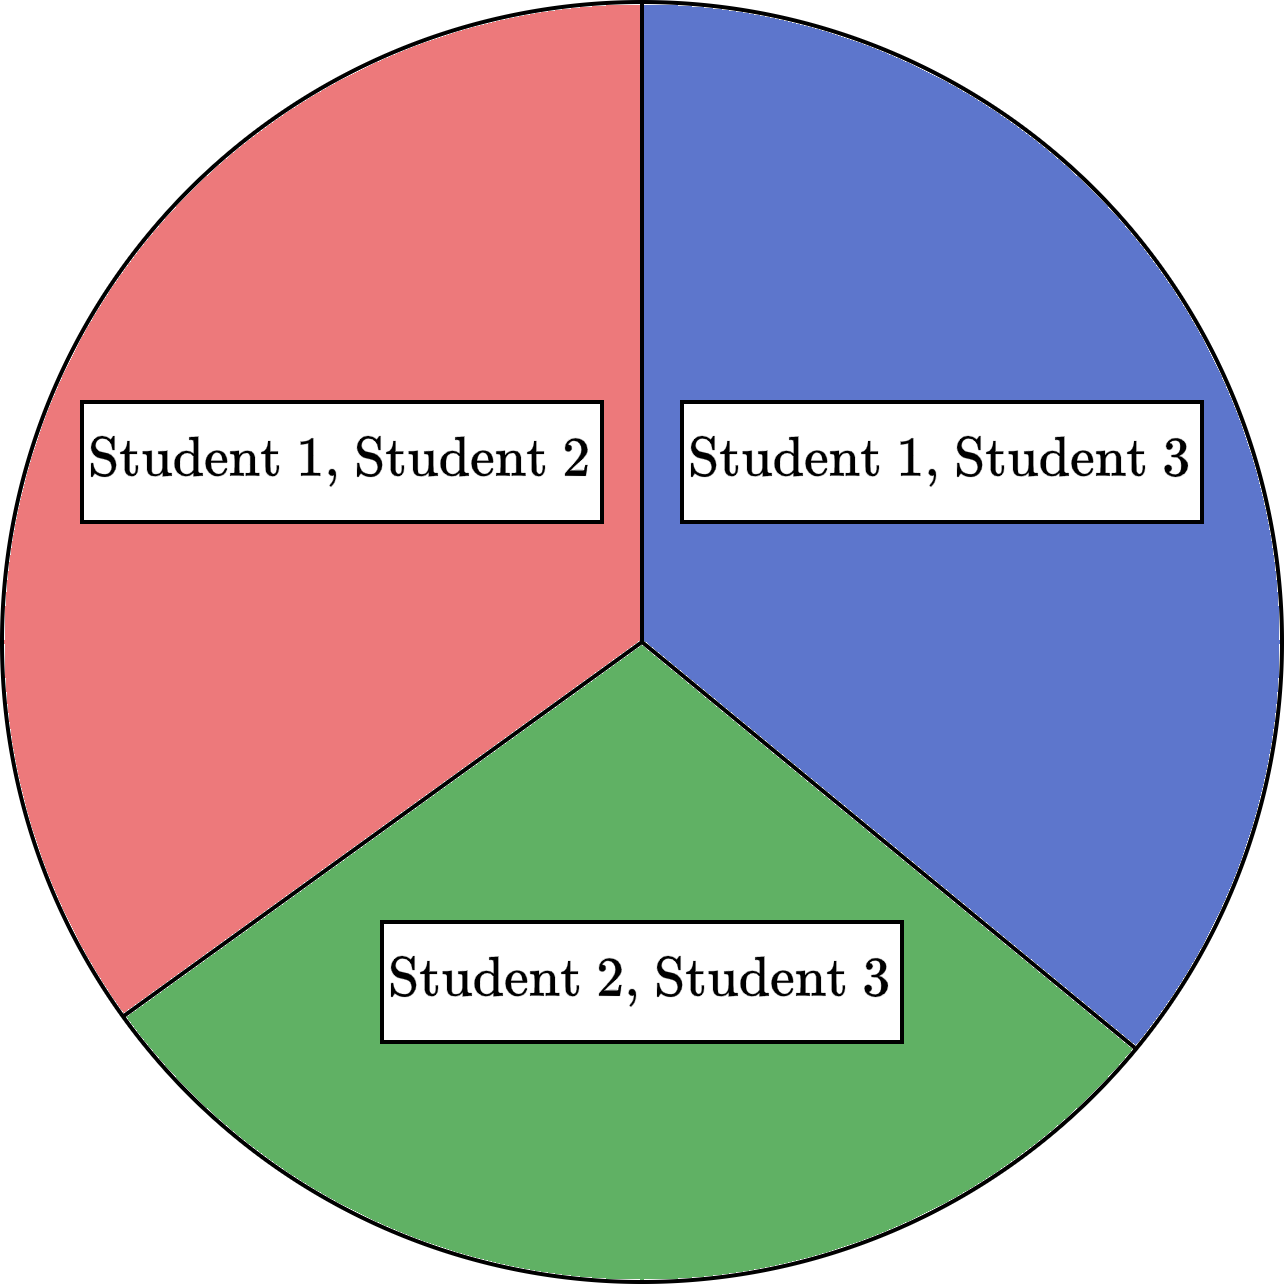
\includegraphics[width=40mm,scale=0.5]{images/nonparametric_images/best_of_three.png}
            \caption*{Every student gets one question wrong, but by majority, they get all three right!}
        \end{figure}

        Despite each student having a \~66\% accuracy, they have a 100\% accuracy together!
            \note{This is a very optimistic version of why bagging could be beneficial. But the idea holds true in general.}

        We call this "bootstrap aggregation", or "bagging".\\

        \begin{concept}
            \vocab{Bagging} is a particular kind of \purp{ensemble method}, combining several models to compute an answer.

            \begin{itemize}
                \item In bagging, we train several models \gren{separately}, and then combine all of their answers, to hopefully find a more \purp{accurate} result. 
            \end{itemize}
        \end{concept}




    \phantom{}
    
    \subsection{Bagging: Bootstrapping (\redd{Optional})}

        So, now, we need to hammer out the details of this process:

        \begin{itemize}
            \item Create \purp{multiple} datasets 

            \item Train a \gren{tree} on each of those datasets

            \item \orgg{Combine} the results of those trees
        \end{itemize}

        First: how do we create multiple datasets from our training data? 

        \begin{itemize}
            \item We could try breaking our data into \purp{chunks}, like we do in cross-validation.
        \end{itemize}

        But that's not what we want here:\\

        \begin{concept}
            In \vocab{bagging}, we don't want to break our data into \gren{chunks} (partitioning).

            This is because these chunks of data aren't independent: they're \orgg{correlated} with each other.

            \begin{itemize}
                \item If you include data point $i$ in chunk $k$, you \purp{know} that data point $i$ \redd{isn't} in chunk $k+1$.

                \item Knowing about one chunk, provides information about the other chunks: that's how you know they're correlated.
            \end{itemize}

            We want each of our models to make its decisions, \orgg{independent} of our other models.
        \end{concept}

        \phantom{}

        \begin{remark*}
            If our chunks of data are correlated, then why do we use \purp{partitioning} for our \vocab{cross-validation}?

            \begin{itemize}
                \item In cross-validation, we want to see how our model performs on data it \orgg{hasn't seen before}.

                \item So, it's important to make sure that the chunk we \gren{train} on, is different from the chunk we \purp{test} on.
            \end{itemize}
        \end{remark*}

        How do we create our datasets, then?

        \begin{itemize}
            \item We \orgg{sample with replacement}: after you sample a data point, you \gren{put it back} in the dataset.

            \item So, you can sample the same data point \purp{multiple times}, or not at all.

            \item Each dataset we make is called a \vocab{bootstrap sample}.\\
        \end{itemize}

        \begin{concept}
            When creating data for \vocab{bagging}, we use \purp{bootstrapping}:

            \begin{itemize}
                \item Each dataset is created by \orgg{sampling with replacement}. This dataset is a \vocab{bootstrap sample}.
            \end{itemize}

            \subsecdiv

            This creates two major benefits:

            \begin{itemize}
                \item Each bootstrap sample is \orgg{uncorrelated}: knowing the data in one dataset, tells you nothing about the others.
                    \begin{itemize}
                        \item That means our trees will be \gren{fully separate} from one another.
                    \end{itemize}

                \item When bootstrapping our dataset, we randomly \purp{modify} it, which helps us account for \gren{estimation error}:

                \begin{itemize}
                    \item Each dataset can end up with multiple of a single data point, or missing several data points.

                    \item So, each tree uses a different "\purp{variation}" of our dataset.
                \end{itemize}
            \end{itemize}
        \end{concept}

        This bootstrapping process, along with "aggregating" opinions across multiple models, is why we call this \vocab{bootstrap aggregating} (shortened to bagging).

        But why do we call it "bootstrapping"?\\

        \begin{remark*}
            Our training data comes from our true distribution. We could say that it was "\orgg{sampled}" from it.

            \begin{itemize}
                \item Meanwhile, our "\vocab{bootstrap sample}" comes from sampling our \orgg{training data}.

                \item In other words, we're \brow{sampling a sample}.
            \end{itemize}

            This is kind of \purp{circular}: we're getting "more data", without actually getting \gren{new} data.

            \subsecdiv

            Thus, we call it \vocab{bootstrapping}, referencing the phrase "pull yourself up by your bootstraps".

            \begin{itemize}
                \item Because, it's circular to try to "pull yourself up".
            \end{itemize}
        \end{remark*}

        Bootstrap sampling is also used for statistical analysis, when our data is limited.

        \begin{itemize}
            \item If we bootstrap from our sample, multiple times, we can compute the \textit{mean} of those bootstraps.

            \item So, rather than just having the single mean of our whole sample, we find multiple possible means we could get from our data.
                \note{This can be useful: for example, suppose that your bootstrap means vary wildly. We might not be able to trust our sample mean, if it changes so easily.}
        \end{itemize}




    \phantom{}

    \subsection{Bagging: Completed}


        We have a procedure for bagging now.\\
        
        \begin{definition}
            \vocab{Bagging} (bootstrap aggregation) is an \purp{ensemble method} for reducing \gren{estimation error}, by combining the answers from $B$ independent models.

            \begin{itemize}
                \item First, we create a \orgg{bootstrap sample} for each tree, sampling with replacement from our dataset $\data$.

                \item We train the $\nth{b}$ tree using the $\nth{b}$ bootstrap. The \purp{predictor} we get from this is written as

                \begin{equation*}
                    \hat{f}^b(x)
                \end{equation*}
            \end{itemize}

            When we're evaluating a particular data point $x$, we use each of our models, and then \orgg{aggregate} the results.

            \begin{itemize}
                \item Regression and classification use different methods of aggregation.
            \end{itemize}
        \end{definition}

        Our "aggregation" method is the same as it was for determining the output of one tree region $R_m$.\\

        \begin{kequation}
            In a \vocab{regression} problem, we aggregate our $B$ trees by \purp{averaging} their results.

            \begin{equation*}
                \hat{y}_{bag}(x) =\quad \frac{1}{B} \sum_b \hat{f}_b(x) \quad = \quad\operatorname{Average}_b \Big( \hat{f}_b(x) \Big)
            \end{equation*}

            In a \vocab{classification} problem, we aggregate our $B$ trees by taking the \gren{majority} (most common) vote.

            \begin{equation*}
                \hat{y}_{bag}(x) = \quad \operatorname{Majority}_b \Big( \hat{f}_b(x) \Big)
            \end{equation*}
        \end{kequation}

        We \textit{hope} that bagging reduces estimation, but does it really? It turns out it does!

        \begin{itemize}
            \item But as a tradeoff, it's not easily interpretable, like a single tree is.
                \note{Imagine having to reference 20 different trees every time you need to make a decision... it's unwieldly.}\\
        \end{itemize}

        \begin{concept}
            Bagging can be shown to \purp{reduce} estimation error.

            \begin{itemize}
                \item So, \vocab{bagged trees} will generally perform \gren{better} than an individual tree.
            \end{itemize}

            \textit{But}, we it's much more difficult to interpret a bagged tree, than a single one.

            \begin{itemize}
                \item You have to look at \gren{several} different trees to understand a decision.
            \end{itemize}
        \end{concept}

            \note{This isn't just saying that, in practice, bagging seems to reduce estimation error. We actually have theoretical results that suggest it should!}




    \pagebreak

    \subsection{Random Forests}

        In bagging, we created several different "opinions" on our data, by training each tree on a modified version of our dataset.

        Here, we'll consider a different approach:

        \begin{itemize}
            \item Instead of modifying our dataset, we'll modify which \orgg{dimensions} we split along.

            \item Each time we make a split, we'll \purp{randomly select} a few dimensions, and only choose the best of those to split along.
                \note{So, if the original "best" splitting dimension is omitted, then the tree will choose the best one it has access to.}
        \end{itemize}

        This time, all of our trees have the \gren{same dataset}, but they split in \purp{randomly different} ways.

        \begin{itemize}
            \item Many trees, modified randomly: we call this a \vocab{random forest}.\\
        \end{itemize}

        \begin{definition}
            The \vocab{random forest} approach is an \purp{ensemble method} where, instead of modifying the data for each tree, we modify the \gren{splitting algorithm} for each tree.

            \begin{itemize}
                \item Normally, when training a tree, it selects the best split, on the best dimension.

                \item But in random forests, we \purp{randomly restrict} our tree to only split along \gren{some dimensions}.
            \end{itemize}

            So, our tree splits the "best dimension", among the ones those that are randomly selected.
        \end{definition}

        Restricting our tree seems counter-intuitive: why would we deliberately prevent it from choosing the best split?

        \begin{itemize}
            \item This forces some of our trees to "\gren{explore}" other splits, which might be worse short-term, but better long-term.

            \item Hopefully, this avoids the \purp{estimation error} problem: by trying lots of trees, we can avoid getting "unlucky" with one tree.
        \end{itemize}

        Random forests often perform remarkably well, compared to many, much fancier methods. 




    \pagebreak

    \subsection{Other types of tree models}

        There are tons of tree variations:

        \begin{itemize}
            \item We could split along \gren{any hyperplane}, rather than restricting ourselves to only one axis.
                \note{For example, we could try $2x_1+3x_2 \geq 0$, rather than $x_1 \geq 10$.}
                \begin{itemize}
                    \item In which case, we have to figure out how to limit our options: there are many more hyperplanes, than ways to split on only one axis.
                \end{itemize}

            \item We could expand beyond hyperplanes: we could use \orgg{polynomial curves}, like paraboloids.
                \note{Similar to our "polynomial features" method.}

            \item We could use \purp{linear regression} for each region $R_m$, rather than just averaging all of our data points.

            \item We could use a \gren{probabilistic} split: rather than a data point belonging in exactly one region, $R_m$, it could \textit{partly} belong to all of them.
                \note{This is called a "hierarchical mixture of experts".}
                
                \begin{itemize}
                    \item \miniex Our data point could 90\% belong to $R_1$, 10\% belong to $R_2$.

                    \item Because this is more continuous than our previous method, we can often use \gren{gradient descent} to train.
                \end{itemize}
        \end{itemize}



    \phantom{}

    \subsection{Benefits of Trees}


        We've shown lots of reasons you might want to use a tree:

        \begin{itemize}
            \item Easy to interpret, fast to train.
            \item Very flexible with different loss functions, problem types.

            \item Often surprisingly effective, despite their simplicity.\\
        \end{itemize}

        \begin{concept}
            It's often good practice to use \gren{trees} as a \vocab{baseline}, to compare more \purp{complex} models against:

            \begin{itemize}
                \item If your complex model doesn't perform much better than a tree, it may not be worth using.
            \end{itemize}
        \end{concept}


\pagebreak

\section{Terms}

    \begin{itemize}
        \item Parametric Methods
        \item Expressive (Review)
        \item Non-parametric methods
        \item $k$-means clustering (Review)
        \item Nearest neighbor
        \item Tree models
        \item Ensembles
        \item Boosting (Optional)
        \item Voronoi Diagram (Optional)
        \item $k$-nearest neighbors (kNN)
        \item Locally weighted regression (Optional)
        \item Distance metric
        \item Euclidean distance (Review)
        \item Manhattan distance (Optional)
        \item Hamming distance (Optional)
        \item Minkowsky distance (Optional)
        \item Binary tree
        \item Root node
        \item Leaf node
        \item Branch
        \item tree model
        \item Partition
        \item Partition function $\pi$
        \item Collection of outputs $O$
        \item Index
        \item Tree model objective function
        \item Greedy algorithm
        \item Early stopping (Review)
        \item Pruning
        \item Low-level/high-level branch
        \item Cost complexity function
        \item Majority function
        \item Misclassification Error
        \item Empirical Probability
        \item Purity
        \item Gini Index 
        \item Information (Optional)
        \item Uncertainty (Optional)
        \item Surprisal (Optional)
        \item Entropy
        \item Information Gain
        \item Ensemble Method
        \item Bagging
        \item Correlated
        \item Bootstrapping
        \item Sampling with Replacement
        \item Random forest
        \item Hierarchical Mixture of Experts
    \end{itemize}